% Options for packages loaded elsewhere
\PassOptionsToPackage{unicode}{hyperref}
\PassOptionsToPackage{hyphens}{url}
\PassOptionsToPackage{dvipsnames,svgnames,x11names}{xcolor}
%
\documentclass[
  letterpaper,
  DIV=11,
  numbers=noendperiod]{scrreprt}

\usepackage{amsmath,amssymb}
\usepackage{lmodern}
\usepackage{iftex}
\ifPDFTeX
  \usepackage[T1]{fontenc}
  \usepackage[utf8]{inputenc}
  \usepackage{textcomp} % provide euro and other symbols
\else % if luatex or xetex
  \usepackage{unicode-math}
  \defaultfontfeatures{Scale=MatchLowercase}
  \defaultfontfeatures[\rmfamily]{Ligatures=TeX,Scale=1}
\fi
% Use upquote if available, for straight quotes in verbatim environments
\IfFileExists{upquote.sty}{\usepackage{upquote}}{}
\IfFileExists{microtype.sty}{% use microtype if available
  \usepackage[]{microtype}
  \UseMicrotypeSet[protrusion]{basicmath} % disable protrusion for tt fonts
}{}
\makeatletter
\@ifundefined{KOMAClassName}{% if non-KOMA class
  \IfFileExists{parskip.sty}{%
    \usepackage{parskip}
  }{% else
    \setlength{\parindent}{0pt}
    \setlength{\parskip}{6pt plus 2pt minus 1pt}}
}{% if KOMA class
  \KOMAoptions{parskip=half}}
\makeatother
\usepackage{xcolor}
\setlength{\emergencystretch}{3em} % prevent overfull lines
\setcounter{secnumdepth}{5}
% Make \paragraph and \subparagraph free-standing
\ifx\paragraph\undefined\else
  \let\oldparagraph\paragraph
  \renewcommand{\paragraph}[1]{\oldparagraph{#1}\mbox{}}
\fi
\ifx\subparagraph\undefined\else
  \let\oldsubparagraph\subparagraph
  \renewcommand{\subparagraph}[1]{\oldsubparagraph{#1}\mbox{}}
\fi

\usepackage{color}
\usepackage{fancyvrb}
\newcommand{\VerbBar}{|}
\newcommand{\VERB}{\Verb[commandchars=\\\{\}]}
\DefineVerbatimEnvironment{Highlighting}{Verbatim}{commandchars=\\\{\}}
% Add ',fontsize=\small' for more characters per line
\usepackage{framed}
\definecolor{shadecolor}{RGB}{241,243,245}
\newenvironment{Shaded}{\begin{snugshade}}{\end{snugshade}}
\newcommand{\AlertTok}[1]{\textcolor[rgb]{0.68,0.00,0.00}{#1}}
\newcommand{\AnnotationTok}[1]{\textcolor[rgb]{0.37,0.37,0.37}{#1}}
\newcommand{\AttributeTok}[1]{\textcolor[rgb]{0.40,0.45,0.13}{#1}}
\newcommand{\BaseNTok}[1]{\textcolor[rgb]{0.68,0.00,0.00}{#1}}
\newcommand{\BuiltInTok}[1]{\textcolor[rgb]{0.00,0.23,0.31}{#1}}
\newcommand{\CharTok}[1]{\textcolor[rgb]{0.13,0.47,0.30}{#1}}
\newcommand{\CommentTok}[1]{\textcolor[rgb]{0.37,0.37,0.37}{#1}}
\newcommand{\CommentVarTok}[1]{\textcolor[rgb]{0.37,0.37,0.37}{\textit{#1}}}
\newcommand{\ConstantTok}[1]{\textcolor[rgb]{0.56,0.35,0.01}{#1}}
\newcommand{\ControlFlowTok}[1]{\textcolor[rgb]{0.00,0.23,0.31}{#1}}
\newcommand{\DataTypeTok}[1]{\textcolor[rgb]{0.68,0.00,0.00}{#1}}
\newcommand{\DecValTok}[1]{\textcolor[rgb]{0.68,0.00,0.00}{#1}}
\newcommand{\DocumentationTok}[1]{\textcolor[rgb]{0.37,0.37,0.37}{\textit{#1}}}
\newcommand{\ErrorTok}[1]{\textcolor[rgb]{0.68,0.00,0.00}{#1}}
\newcommand{\ExtensionTok}[1]{\textcolor[rgb]{0.00,0.23,0.31}{#1}}
\newcommand{\FloatTok}[1]{\textcolor[rgb]{0.68,0.00,0.00}{#1}}
\newcommand{\FunctionTok}[1]{\textcolor[rgb]{0.28,0.35,0.67}{#1}}
\newcommand{\ImportTok}[1]{\textcolor[rgb]{0.00,0.46,0.62}{#1}}
\newcommand{\InformationTok}[1]{\textcolor[rgb]{0.37,0.37,0.37}{#1}}
\newcommand{\KeywordTok}[1]{\textcolor[rgb]{0.00,0.23,0.31}{#1}}
\newcommand{\NormalTok}[1]{\textcolor[rgb]{0.00,0.23,0.31}{#1}}
\newcommand{\OperatorTok}[1]{\textcolor[rgb]{0.37,0.37,0.37}{#1}}
\newcommand{\OtherTok}[1]{\textcolor[rgb]{0.00,0.23,0.31}{#1}}
\newcommand{\PreprocessorTok}[1]{\textcolor[rgb]{0.68,0.00,0.00}{#1}}
\newcommand{\RegionMarkerTok}[1]{\textcolor[rgb]{0.00,0.23,0.31}{#1}}
\newcommand{\SpecialCharTok}[1]{\textcolor[rgb]{0.37,0.37,0.37}{#1}}
\newcommand{\SpecialStringTok}[1]{\textcolor[rgb]{0.13,0.47,0.30}{#1}}
\newcommand{\StringTok}[1]{\textcolor[rgb]{0.13,0.47,0.30}{#1}}
\newcommand{\VariableTok}[1]{\textcolor[rgb]{0.07,0.07,0.07}{#1}}
\newcommand{\VerbatimStringTok}[1]{\textcolor[rgb]{0.13,0.47,0.30}{#1}}
\newcommand{\WarningTok}[1]{\textcolor[rgb]{0.37,0.37,0.37}{\textit{#1}}}

\providecommand{\tightlist}{%
  \setlength{\itemsep}{0pt}\setlength{\parskip}{0pt}}\usepackage{longtable,booktabs,array}
\usepackage{calc} % for calculating minipage widths
% Correct order of tables after \paragraph or \subparagraph
\usepackage{etoolbox}
\makeatletter
\patchcmd\longtable{\par}{\if@noskipsec\mbox{}\fi\par}{}{}
\makeatother
% Allow footnotes in longtable head/foot
\IfFileExists{footnotehyper.sty}{\usepackage{footnotehyper}}{\usepackage{footnote}}
\makesavenoteenv{longtable}
\usepackage{graphicx}
\makeatletter
\def\maxwidth{\ifdim\Gin@nat@width>\linewidth\linewidth\else\Gin@nat@width\fi}
\def\maxheight{\ifdim\Gin@nat@height>\textheight\textheight\else\Gin@nat@height\fi}
\makeatother
% Scale images if necessary, so that they will not overflow the page
% margins by default, and it is still possible to overwrite the defaults
% using explicit options in \includegraphics[width, height, ...]{}
\setkeys{Gin}{width=\maxwidth,height=\maxheight,keepaspectratio}
% Set default figure placement to htbp
\makeatletter
\def\fps@figure{htbp}
\makeatother
\newlength{\cslhangindent}
\setlength{\cslhangindent}{1.5em}
\newlength{\csllabelwidth}
\setlength{\csllabelwidth}{3em}
\newlength{\cslentryspacingunit} % times entry-spacing
\setlength{\cslentryspacingunit}{\parskip}
\newenvironment{CSLReferences}[2] % #1 hanging-ident, #2 entry spacing
 {% don't indent paragraphs
  \setlength{\parindent}{0pt}
  % turn on hanging indent if param 1 is 1
  \ifodd #1
  \let\oldpar\par
  \def\par{\hangindent=\cslhangindent\oldpar}
  \fi
  % set entry spacing
  \setlength{\parskip}{#2\cslentryspacingunit}
 }%
 {}
\usepackage{calc}
\newcommand{\CSLBlock}[1]{#1\hfill\break}
\newcommand{\CSLLeftMargin}[1]{\parbox[t]{\csllabelwidth}{#1}}
\newcommand{\CSLRightInline}[1]{\parbox[t]{\linewidth - \csllabelwidth}{#1}\break}
\newcommand{\CSLIndent}[1]{\hspace{\cslhangindent}#1}

<script src="site_libs/font-awesome-5.13.0/js/script.js"></script>
\KOMAoption{captions}{tableheading}
\makeatletter
\makeatother
\makeatletter
\@ifpackageloaded{bookmark}{}{\usepackage{bookmark}}
\makeatother
\makeatletter
\@ifpackageloaded{caption}{}{\usepackage{caption}}
\AtBeginDocument{%
\ifdefined\contentsname
  \renewcommand*\contentsname{Table of contents}
\else
  \newcommand\contentsname{Table of contents}
\fi
\ifdefined\listfigurename
  \renewcommand*\listfigurename{List of Figures}
\else
  \newcommand\listfigurename{List of Figures}
\fi
\ifdefined\listtablename
  \renewcommand*\listtablename{List of Tables}
\else
  \newcommand\listtablename{List of Tables}
\fi
\ifdefined\figurename
  \renewcommand*\figurename{Figure}
\else
  \newcommand\figurename{Figure}
\fi
\ifdefined\tablename
  \renewcommand*\tablename{Table}
\else
  \newcommand\tablename{Table}
\fi
}
\@ifpackageloaded{float}{}{\usepackage{float}}
\floatstyle{ruled}
\@ifundefined{c@chapter}{\newfloat{codelisting}{h}{lop}}{\newfloat{codelisting}{h}{lop}[chapter]}
\floatname{codelisting}{Listing}
\newcommand*\listoflistings{\listof{codelisting}{List of Listings}}
\usepackage{amsthm}
\theoremstyle{definition}
\newtheorem{exercise}{Exercise}[chapter]
\theoremstyle{remark}
\renewcommand*{\proofname}{Proof}
\newtheorem*{remark}{Remark}
\newtheorem*{solution}{Solution}
\makeatother
\makeatletter
\@ifpackageloaded{caption}{}{\usepackage{caption}}
\@ifpackageloaded{subcaption}{}{\usepackage{subcaption}}
\makeatother
\makeatletter
\@ifpackageloaded{tcolorbox}{}{\usepackage[many]{tcolorbox}}
\makeatother
\makeatletter
\@ifundefined{shadecolor}{\definecolor{shadecolor}{rgb}{.97, .97, .97}}
\makeatother
\makeatletter
\makeatother
\ifLuaTeX
  \usepackage{selnolig}  % disable illegal ligatures
\fi
\IfFileExists{bookmark.sty}{\usepackage{bookmark}}{\usepackage{hyperref}}
\IfFileExists{xurl.sty}{\usepackage{xurl}}{} % add URL line breaks if available
\urlstyle{same} % disable monospaced font for URLs
\hypersetup{
  pdftitle={SOS2901 Maskinlæring for samfunnsvitere},
  pdfauthor={Torbjørn Skardhamar},
  colorlinks=true,
  linkcolor={blue},
  filecolor={Maroon},
  citecolor={Blue},
  urlcolor={Blue},
  pdfcreator={LaTeX via pandoc}}

\title{SOS2901 Maskinlæring for samfunnsvitere}
\usepackage{etoolbox}
\makeatletter
\providecommand{\subtitle}[1]{% add subtitle to \maketitle
  \apptocmd{\@title}{\par {\large #1 \par}}{}{}
}
\makeatother
\subtitle{Oppgaver til hver undervisningsuke}
\author{Torbjørn Skardhamar}
\date{1/7/23}

\begin{document}
\maketitle
\ifdefined\Shaded\renewenvironment{Shaded}{\begin{tcolorbox}[borderline west={3pt}{0pt}{shadecolor}, frame hidden, boxrule=0pt, sharp corners, interior hidden, breakable, enhanced]}{\end{tcolorbox}}\fi

\renewcommand*\contentsname{Table of contents}
{
\hypersetup{linkcolor=}
\setcounter{tocdepth}{2}
\tableofcontents
}
\bookmarksetup{startatroot}

\hypertarget{introduksjon}{%
\chapter*{Introduksjon}\label{introduksjon}}
\addcontentsline{toc}{chapter}{Introduksjon}

\markboth{Introduksjon}{Introduksjon}

Dette dokumentet gir en oversikt over hva vi skal dekke i løpet av
semesteret. Det lages delvis underveis, så det vil bli oppdateringer
jevnlig. Antakeligvis er det enklest å navigere i denne nettsiden, men
du kan også laste ned en pdf-versjon .

(Dessuten skriver jeg disse oppgavene i Quarto som jeg ikke er så god i,
så jeg prøver meg litt frem. Det kan derfor hende layout og andre ting
endres underveis. Bær over med meg!)

Hvert kapittel i dette heftet starter med en gjennomgang av aktuell
teknikk og de kodene som trengs for å gjøre det dere skal. Det vises
gjennom eksempler med et datasett.

Alle datasettene vi skal bruke finner dere imidletid i Canvas under
fanen for Filer. Last de ned til egen masking for å jobbe med dem. Hver
uke skal du gjøre følgende:

\begin{enumerate}
\def\labelenumi{\arabic{enumi})}
\tightlist
\item
  Gå gjennom eksempelet og sjekke at du klarer reprodusere resultatene
  og skjønner omtrentlig hva du driver med.
\item
  Velg et av de andre datasettene og gjør tilsvarende analyser med dette
\end{enumerate}

\emph{Forberedelse til undervisning} Til hver undervisningsgang skal du
ha forberedt to ting:

\begin{enumerate}
\def\labelenumi{\arabic{enumi})}
\tightlist
\item
  Valgt et datasett og splittet dette i training/testing
\item
  Formulert noe om hva en prediksjon med denne typen data kan tenkes å
  brukes til i praksis (en slags problemstilling, med andre ord)
\item
  Forberede minst ett spørsmål eller kommentar til det tekniske eller
  pensum. Vi starter hver undervisning med oppklaringer
\end{enumerate}

\bookmarksetup{startatroot}

\hypertarget{r-og-rstudio}{%
\chapter*{R og Rstudio}\label{r-og-rstudio}}
\addcontentsline{toc}{chapter}{R og Rstudio}

\markboth{R og Rstudio}{R og Rstudio}

\hypertarget{installasjon}{%
\section*{Installasjon}\label{installasjon}}
\addcontentsline{toc}{section}{Installasjon}

\markright{Installasjon}

Du må installere både \href{https://www.r-project.org/}{R} og
\href{https://posit.co/products/open-source/rstudio/}{Rstudio} på din
datamaskin. Hvis du har Windows-maskin trenger du også installere
\href{https://cran.r-project.org/bin/windows/Rtools/rtools42/rtools.html}{Rtools}.
Hvis du har Mac OS X kan det hende du må installere
\href{https://www.xquartz.org/}{XQuartz}.

Se ellers video fra \href{https://youtu.be/ulIv0NiVTs4}{SICSS}

\url{https://youtu.be/ulIv0NiVTs4}

\hypertarget{pakker}{%
\section*{Pakker}\label{pakker}}
\addcontentsline{toc}{section}{Pakker}

\markright{Pakker}

R er basert på bruk av ``pakker'' som må installeres for å få tilgang
til funksjoner vi skal bruke. Disse installeres med bruk av kommandoen
\texttt{install.packages()}. F.eks. kan man installere pakken Tidyverse
med følgende: \texttt{install.packages("tidyverse")}.

For å installere flere pakker kan man kjøre \texttt{install.packages()}
flere ganger, men det er enklere å liste opp alle pakkene i et objekt og
så kjøre \texttt{install.packages()} på dette objektet. Noe slikt:

\begin{Shaded}
\begin{Highlighting}[]
\NormalTok{pkgs }\OtherTok{\textless{}{-}} \FunctionTok{c}\NormalTok{(}\StringTok{"tidyverse"}\NormalTok{, }\StringTok{"skimr"}\NormalTok{, }\StringTok{"randomForest"}\NormalTok{)}
\CommentTok{\#install.packages(pkgs)}
\end{Highlighting}
\end{Shaded}

Men for at du skal kunne bruke pakkene må du aktivere dem i R ved
\texttt{library()}. Dette må du gjøre hver gang du starter opp R. Det
kan se slik ut:

\begin{Shaded}
\begin{Highlighting}[]
\FunctionTok{library}\NormalTok{(tidyverse)}
\FunctionTok{library}\NormalTok{(skimr)}
\FunctionTok{library}\NormalTok{(randomForest)}
\FunctionTok{library}\NormalTok{(caret)}
\FunctionTok{library}\NormalTok{(AUC)}
\end{Highlighting}
\end{Shaded}

\hypertarget{forutsetninger}{%
\section*{Forutsetninger}\label{forutsetninger}}
\addcontentsline{toc}{section}{Forutsetninger}

\markright{Forutsetninger}

Dette kurset forutsetter at man har grunnleggende ferdigheter i
kvantitative metoder og har brukt \emph{R} før. Hvis du vet du trenger
det: frisk opp litt fra tidligere kurs.

Når det er sagt, så er det begrenset hvor mye man \emph{må} kunne fra
før hvis du er motivert til å jobbe med stoffet skal du nok få til
dette. Det blir mye nytt uansett.

Hvis du trenger oppfriskning av hvordan R fungerer, så er Wickham \&
Grolemunds bok \href{https://r4ds.had.co.nz/}{``R for data science''} et
utmerket oppslagsverk. Men merk at vi i begrenset grad vil bruke
``Tidyverse'' til annet enn datahåndtering og noe grafikk.

\bookmarksetup{startatroot}

\hypertarget{introduksjon-til-maskinluxe6ring}{%
\chapter{Introduksjon til
maskinlæring}\label{introduksjon-til-maskinluxe6ring}}

Temaet for denne forelesningen er maskinlæring generelt og datadrevne
beslutninger. Vi kommer inn på flere av temaene som vil behandles
grundigere gjennom kurset.

Hvert kapittel starter med en introduksjon til temaet og et empirisk
eksempel. Deretter kommer noen oppgaver, som dere skal løse. Oppgavene
er ganske åpne og det er meningen at dere skal velge et annet datasett
og gjøre tilsvarende analyser som i eksempelet. Fra eksempelet får dere
også nødvendig kode.

\hypertarget{oppgaver}{%
\section{Oppgaver}\label{oppgaver}}

\leavevmode\vadjust pre{\hypertarget{exr-sepaa}{}}%
\begin{exercise}[]\label{exr-sepaa}

Kan man tenke seg målrettede tiltak som \textbf{ikke} innebærer en form
for prediksjon om fremtiden? (Implisitt eller eksplisitt)

\end{exercise}

\leavevmode\vadjust pre{\hypertarget{exr-feil}{}}%
\begin{exercise}[]\label{exr-feil}

Hvor alvorlig er det å gjøre feil? Hva avgjør om feil prediksjon spiller
noen rolle?

\end{exercise}

\bookmarksetup{startatroot}

\hypertarget{noen-innledende-metodiske-begrep}{%
\chapter{Noen innledende metodiske
begrep}\label{noen-innledende-metodiske-begrep}}

I standard samfunnsvitenskapelige metodekurs lærer man først og fremst
teknikker for å beskrive data og statistisk inferens for å beskrive
usikkerheten rundt estimatene. Avhengig av studiets øvrige design kan
resultatene tolkes kausalt og/eller generalisere til en nærmere
veldefinert populasjon (Berk 2016).

Usikkerhet beskrives typisk ved hjelp standardfeil, p-verdier og
konfidensintervall tilhørende spesifikke statistiske tester. Dette
innebærer at man bruker statistiske \emph{modeller} for hvordan
resultatene ville sett ut under spesifikke forutsetninger.
Samplingfordelinger som normalfordelingen og en del andre tilsvarende
fordelinger er derfor sentralt. De fleste teknikkene vi skal bruke i
dette kurset er \emph{ikke} statistiske modeller i samme forstand og det
er ingen antakelser om samplingfordelinger. Standardfeil og
konfidensintervall kan derfor ikke regnes ut. Usikkerhet og hvem
resultatene gjelder for er også relevante for maskinlæring, men ikke
helt på samme måte.

\hypertarget{forklaringer-og-prediksjoner}{%
\section{Forklaringer og
prediksjoner}\label{forklaringer-og-prediksjoner}}

Vi er i liten grad interessert i regresjonskoeffisienter, \(\beta\), og
tolkning av denne. Derimot er vi interessert i det predikerte utfallet
\(\hat{y}_i\).

\hypertarget{overfitting-training-og-testing-dataset}{%
\section{Overfitting: training og testing
dataset}\label{overfitting-training-og-testing-dataset}}

Når man tilpasser en statistisk modell eller algoritme til data så er
det lett å tenke at modellen bør gjenspeile dataene så godt som mulig.
Samtidig sies det ofte at modellene skal være så enkle som tilrådelig.
En mer komplisert modell vil jo være i stand til å tilpasses dataene i
større grad, så hvordan avveie dette?

Spørsmålet nå er ikke hvor godt modellen passer til disse dataene, men
hvordan den passer til \emph{nye} data! Altså \emph{fremtidige} data
eller fremtidig situasjon. La oss si at vi har et datasett som kan
plottes om følger:

\begin{Shaded}
\begin{Highlighting}[]
\FunctionTok{library}\NormalTok{(tidyverse)}
\end{Highlighting}
\end{Shaded}

\begin{verbatim}
-- Attaching packages --------------------------------------- tidyverse 1.3.2 --
v ggplot2 3.4.0      v purrr   0.3.5 
v tibble  3.1.8      v dplyr   1.0.10
v tidyr   1.2.1      v stringr 1.4.1 
v readr   2.1.3      v forcats 0.5.2 
-- Conflicts ------------------------------------------ tidyverse_conflicts() --
x dplyr::filter() masks stats::filter()
x dplyr::lag()    masks stats::lag()
\end{verbatim}

\begin{Shaded}
\begin{Highlighting}[]
\NormalTok{n }\OtherTok{\textless{}{-}} \DecValTok{10}
\NormalTok{beta }\OtherTok{\textless{}{-}} \DecValTok{1}
\FunctionTok{set.seed}\NormalTok{(}\DecValTok{42}\NormalTok{)}
\NormalTok{x }\OtherTok{\textless{}{-}} \FunctionTok{round}\NormalTok{(}\DecValTok{20} \SpecialCharTok{+} \FunctionTok{runif}\NormalTok{(n)}\SpecialCharTok{*}\DecValTok{50}\NormalTok{, }\AttributeTok{digits =} \DecValTok{1}\NormalTok{)}
\NormalTok{y }\OtherTok{\textless{}{-}} \DecValTok{1} \SpecialCharTok{+}\NormalTok{ beta}\SpecialCharTok{*}\NormalTok{x }\SpecialCharTok{+} \FunctionTok{rnorm}\NormalTok{(n)}\SpecialCharTok{*}\DecValTok{10}

\NormalTok{df }\OtherTok{\textless{}{-}} \FunctionTok{data.frame}\NormalTok{(}\AttributeTok{x =}\NormalTok{ x, }\AttributeTok{y =}\NormalTok{ y) }\SpecialCharTok{\%\textgreater{}\%} 
  \FunctionTok{mutate}\NormalTok{(}\AttributeTok{d =} \FunctionTok{case\_when}\NormalTok{(x }\SpecialCharTok{\textless{}} \DecValTok{50} \SpecialCharTok{\textasciitilde{}} \DecValTok{0}\NormalTok{,}
\NormalTok{                       x }\SpecialCharTok{\textless{}} \DecValTok{56} \SpecialCharTok{\textasciitilde{}} \DecValTok{1}\NormalTok{, }
                       \ConstantTok{TRUE} \SpecialCharTok{\textasciitilde{}}\DecValTok{2}\NormalTok{) }\SpecialCharTok{\%\textgreater{}\%} \FunctionTok{as\_factor}\NormalTok{())}


\NormalTok{g1 }\OtherTok{\textless{}{-}} \FunctionTok{ggplot}\NormalTok{(df, }\FunctionTok{aes}\NormalTok{(}\AttributeTok{x =}\NormalTok{ x, }\AttributeTok{y =}\NormalTok{ y)) }\SpecialCharTok{+}
  \FunctionTok{geom\_point}\NormalTok{() }
\NormalTok{g1}
\end{Highlighting}
\end{Shaded}

\begin{figure}[H]

{\centering 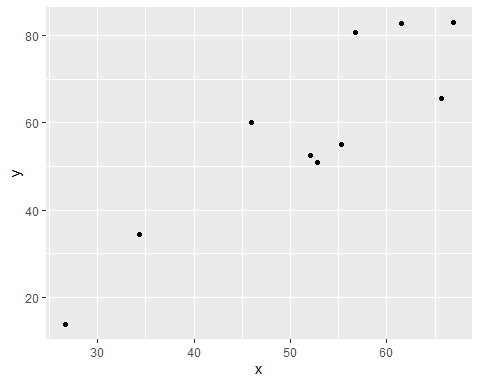
\includegraphics{./grunnleggendeML_files/figure-pdf/unnamed-chunk-1-1.pdf}

}

\end{figure}

Vi kunne her tilpasse en enkel lineær regresjonsmodell eller en mer
komplisert modell. Resultatet vises i grafen nedenfor.

\begin{Shaded}
\begin{Highlighting}[]
\NormalTok{est1 }\OtherTok{\textless{}{-}} \FunctionTok{lm}\NormalTok{(y }\SpecialCharTok{\textasciitilde{}}\NormalTok{ x }\SpecialCharTok{+}\NormalTok{ x}\SpecialCharTok{*}\NormalTok{d, }\AttributeTok{data =}\NormalTok{ df)}
\NormalTok{est2 }\OtherTok{\textless{}{-}} \FunctionTok{lm}\NormalTok{(y }\SpecialCharTok{\textasciitilde{}}\NormalTok{ x, }\AttributeTok{data =}\NormalTok{ df)}

\NormalTok{df\_p1 }\OtherTok{\textless{}{-}}\NormalTok{ df }\SpecialCharTok{\%\textgreater{}\%} 
  \FunctionTok{mutate}\NormalTok{(}\AttributeTok{pred =} \FunctionTok{predict}\NormalTok{(est1))  }\SpecialCharTok{\%\textgreater{}\%} 
  \FunctionTok{mutate}\NormalTok{(}\AttributeTok{res\_pred =}\NormalTok{ y }\SpecialCharTok{{-}}\NormalTok{ pred, }
         \AttributeTok{res\_y =}\NormalTok{ y }\SpecialCharTok{{-}} \FunctionTok{mean}\NormalTok{(y))}

\NormalTok{df\_p1 }\SpecialCharTok{\%\textgreater{}\%} 
  \FunctionTok{summarise}\NormalTok{(}\AttributeTok{res\_pred =} \FunctionTok{sum}\NormalTok{(res\_pred}\SpecialCharTok{\^{}}\DecValTok{2}\NormalTok{), }
            \AttributeTok{res\_y =} \FunctionTok{sum}\NormalTok{(res\_y}\SpecialCharTok{\^{}}\DecValTok{2}\NormalTok{)) }\SpecialCharTok{\%\textgreater{}\%} 
  \FunctionTok{mutate}\NormalTok{(}\DecValTok{1} \SpecialCharTok{{-}}\NormalTok{ res\_pred}\SpecialCharTok{/}\NormalTok{res\_y)}
\end{Highlighting}
\end{Shaded}

\begin{verbatim}
  res_pred    res_y 1 - res_pred/res_y
1 190.8017 4411.586          0.9567499
\end{verbatim}

\begin{Shaded}
\begin{Highlighting}[]
\FunctionTok{ggplot}\NormalTok{(df, }\FunctionTok{aes}\NormalTok{(}\AttributeTok{x =}\NormalTok{ x, }\AttributeTok{y =}\NormalTok{ y)) }\SpecialCharTok{+}
  \FunctionTok{geom\_point}\NormalTok{(}\AttributeTok{col =} \StringTok{"black"}\NormalTok{) }\SpecialCharTok{+}
  \FunctionTok{geom\_line}\NormalTok{(}\AttributeTok{data =}\NormalTok{ df\_p1, }\FunctionTok{aes}\NormalTok{(}\AttributeTok{y =}\NormalTok{ pred), }\AttributeTok{col =} \StringTok{"red"}\NormalTok{, }\AttributeTok{linewidth =}\NormalTok{ .}\DecValTok{7}\NormalTok{) }\SpecialCharTok{+}
  \FunctionTok{stat\_smooth}\NormalTok{(}\AttributeTok{method=}\StringTok{\textquotesingle{}lm\textquotesingle{}}\NormalTok{, }\AttributeTok{formula =}\NormalTok{ y }\SpecialCharTok{\textasciitilde{}}\NormalTok{ x, }\AttributeTok{se =}\NormalTok{ F, }\AttributeTok{col =} \StringTok{"blue"}\NormalTok{, }\AttributeTok{linewidth =}\NormalTok{ .}\DecValTok{7}\NormalTok{)}
\end{Highlighting}
\end{Shaded}

\begin{figure}[H]

{\centering \includegraphics{./grunnleggendeML_files/figure-pdf/unnamed-chunk-2-1.pdf}

}

\end{figure}

Den kompliserte modellen gir \(r^2\) = 0.9567499 mens den enkle lineære
gir \(r^2\) = 0.8066771.

\begin{Shaded}
\begin{Highlighting}[]
\FunctionTok{summary}\NormalTok{(est1)}\SpecialCharTok{$}\NormalTok{r.squared}
\end{Highlighting}
\end{Shaded}

\begin{verbatim}
[1] 0.9567499
\end{verbatim}

\begin{Shaded}
\begin{Highlighting}[]
\FunctionTok{summary}\NormalTok{(est2)}\SpecialCharTok{$}\NormalTok{r.squared}
\end{Highlighting}
\end{Shaded}

\begin{verbatim}
[1] 0.8066771
\end{verbatim}

\begin{Shaded}
\begin{Highlighting}[]
\NormalTok{x }\OtherTok{\textless{}{-}} \FunctionTok{round}\NormalTok{(}\DecValTok{20} \SpecialCharTok{+} \FunctionTok{runif}\NormalTok{(n)}\SpecialCharTok{*}\DecValTok{50}\NormalTok{, }\AttributeTok{digits =} \DecValTok{1}\NormalTok{)}
\NormalTok{y }\OtherTok{\textless{}{-}} \DecValTok{1} \SpecialCharTok{+}\NormalTok{ beta}\SpecialCharTok{*}\NormalTok{x }\SpecialCharTok{+} \FunctionTok{rnorm}\NormalTok{(n)}\SpecialCharTok{*}\DecValTok{10}
\NormalTok{df2 }\OtherTok{\textless{}{-}} \FunctionTok{data.frame}\NormalTok{(}\AttributeTok{x =}\NormalTok{ x, }\AttributeTok{y =}\NormalTok{ y)}
  
\NormalTok{g1 }\SpecialCharTok{+}
  \FunctionTok{geom\_point}\NormalTok{(}\AttributeTok{data =}\NormalTok{ df2, }\AttributeTok{col =} \StringTok{"blue"}\NormalTok{) }\SpecialCharTok{+}
  \FunctionTok{geom\_smooth}\NormalTok{(}\AttributeTok{method =}\NormalTok{ lm, }\AttributeTok{se =}\NormalTok{ F, }\AttributeTok{col =} \StringTok{"red"}\NormalTok{)}
\end{Highlighting}
\end{Shaded}

\begin{verbatim}
`geom_smooth()` using formula = 'y ~ x'
\end{verbatim}

\begin{figure}[H]

{\centering \includegraphics{./grunnleggendeML_files/figure-pdf/unnamed-chunk-4-1.pdf}

}

\end{figure}

\hypertarget{klassifikasjonsusikkerhet---grunnleggende-begreper}{%
\section{Klassifikasjonsusikkerhet - grunnleggende
begreper}\label{klassifikasjonsusikkerhet---grunnleggende-begreper}}

\hypertarget{falske-positive-og-negative}{%
\subsection{falske positive og
negative}\label{falske-positive-og-negative}}

Når vi predikerer et kategorisk utfall er det gjerne ett av utfallene vi
primært er interessert i. Disse kalles \emph{positive} og de andre er
\emph{negative}. Dette har ingenting å gjøre med om utfallet er bra
eller dårlig å gjøre. Å predikere en sykdom vil være \emph{positivt} og
å være frisk vil være \emph{negativt}. Å ha tilbakefall til kriminalitet
vil være \emph{positivt} og lovlydig vil være \emph{negativt}.

En \emph{positiv} prediksjon kan da være korrekt eller feil, og disse
kalles da henholdsvis \emph{sanne} eller \emph{falske} positive.
Tilsvarende kan en negaitv prediksjon være sann eller falsk.

\hypertarget{confusion-matrix}{%
\subsection{Confusion matrix}\label{confusion-matrix}}

\hypertarget{asymetriske-kostnader}{%
\subsection{Asymetriske kostnader}\label{asymetriske-kostnader}}

\hypertarget{rettferdighet-og-rimelighet}{%
\section{Rettferdighet og
rimelighet}\label{rettferdighet-og-rimelighet}}

I diskusjoner av anvendelser av maskinlæring står rettferdighet helt
sentralt. Men det er ikke alltid like klart hva dette egentlig betyr
utover at det er forskjellsbehandling. Tross alt er hele formålet med
prediksjon å nettopp forskjellsbehandle, eller \emph{målrette} som det
også kan kalles.

\hypertarget{fundamentale-skjvheter-i-data}{%
\subsection{Fundamentale skjvheter i
data}\label{fundamentale-skjvheter-i-data}}

Siden maskinlæring baserer seg på å lære av tilgjengelige data for å
benytte det på nye tilfeller spiller det vesentlig rolle hvordan de
opprinnelige dataene ble generert i utgangspunktet.

Et velkjent eksempel er hvordan
\href{https://www.reuters.com/article/us-amazon-com-jobs-automation-insight-idUSKCN1MK08G}{Amazon
besluttet å slutte å bruke en algoritme for rekruttering fordi den
systematisk valgte bort kvinner}. Grunnen til at algoritmen gjorde dette
var så enkelt som at dataene den var trent opp på var mannsdominert.
Algoritmen hadde altså primært tilgang til informasjon om hvilke
egenskaper som kjennetegnet talentfulle \emph{mannlige} kandidater, som
altså kan være forskjellige fra talentfulle \emph{kvinnelige}
kandidater.

Når man skal ta en algoritme i bruk er det derfor helt avgjørende at man
kan forsvare bruken av de dataene algoritmen er trent på. Kjente
skjevheter kan i prinsippet motarbeides ved \emph{tuning} (dette kommer
vi tilbake til), men det er vanskelig å garantere at det er skjevheter
man \emph{ikke} har tenkt på.

\hypertarget{urimelige-feilrater}{%
\subsection{Urimelige feilrater}\label{urimelige-feilrater}}

\hypertarget{ulike-feilrater-puxe5-tvers-av-undergrupper}{%
\subsection{Ulike feilrater på tvers av
undergrupper}\label{ulike-feilrater-puxe5-tvers-av-undergrupper}}

\bookmarksetup{startatroot}

\hypertarget{lineuxe6r-regresjon}{%
\chapter{Lineær regresjon}\label{lineuxe6r-regresjon}}

\hypertarget{ols-i-r}{%
\section{OLS i R}\label{ols-i-r}}

Vi illustrerer lineær regresjon med et empirisk eksempel. Her skal vi
bruke data for norske kommuner i 2016. La oss si at vi er interessert i
hvordan antall voldshendelser per 1000 innbyggere vil endre seg i en
kommune. Dette kunne være relevant for langtidsplanlegging av
forebygging, politibemanning, helsetjenester osv. Det kan være et område
som er i stor endring slik at befolkningssammensetningen forventes å
endre seg og/eller det er endrede lokale økonomiske utsikter.

Først leser vi inn dataene og tar en titt på variabellisten.

\begin{Shaded}
\begin{Highlighting}[]
\FunctionTok{load}\NormalTok{(}\StringTok{"../data/kom\_2016.RData"}\NormalTok{)}
\FunctionTok{glimpse}\NormalTok{(kom\_2016)}
\end{Highlighting}
\end{Shaded}

\begin{verbatim}
Rows: 643
Columns: 19
$ kommune                 <chr> "0101", "0104", "0105", "0106", "0111", "0119"~
$ year                    <dbl> 2015, 2015, 2015, 2015, 2015, 2015, 2015, 2015~
$ bef_tot                 <int> 30328, 31802, 54192, 78159, 4480, 3613, 5346, ~
$ prop_unge_menn          <dbl> 0.11890003, 0.11533866, 0.11776646, 0.11705626~
$ prop_kvinner_16_18      <dbl> 0.01869559, 0.01870952, 0.01967080, 0.01939636~
$ prop_menn_16_18         <dbl> 0.01945397, 0.01911829, 0.01950472, 0.02020241~
$ prop_menn_19_34         <dbl> 0.09944606, 0.09622036, 0.09826174, 0.09685385~
$ prop_kvinner_19_34      <dbl> 0.09502770, 0.08993145, 0.09386994, 0.09366804~
$ prop_shj_mottakere      <dbl> 0.03900686, 0.03631847, 0.02804842, 0.02552489~
$ prop_shj_mottakere_6mnd <dbl> 0.013782643, 0.013018049, 0.011883673, 0.00996~
$ gj_innt_17_34           <int> 243200, 235100, 250600, 244300, 229700, 237500~
$ gj_innt_35_66           <int> 475800, 511100, 473400, 500700, 540200, 507300~
$ gj_innt_alle            <int> 380500, 405300, 381400, 396600, 434400, 390600~
$ lovb_ialt               <dbl> 108.8, 77.1, 66.5, 70.4, 59.2, 137.3, 66.8, 44~
$ Orden                   <dbl> 18.7, 9.2, 9.6, 8.8, 4.2, 16.3, 24.7, 5.4, 9.1~
$ Rusmiddellovbrudd       <dbl> 21.7, 14.6, 12.3, 10.3, 4.0, 29.9, 11.2, 3.9, ~
$ Trafikkovertredelse     <dbl> 14.2, 7.9, 9.6, 8.0, 5.1, 24.9, 7.9, 11.8, 8.2~
$ Vold                    <dbl> 10.4, 8.1, 6.8, 7.4, 7.6, 5.3, 7.7, 5.4, 8.4, ~
$ lovb_annet              <dbl> 24.5, 10.3, 8.6, 10.1, 17.9, 49.3, 8.2, 8.3, 1~
\end{verbatim}

En annen måte å få oversikt over dataene på er å bruke funksjonen
\texttt{skim()}, som gir noe mer informasjon om fordelingen av hver
enkelt variabel.

\begin{Shaded}
\begin{Highlighting}[]
\FunctionTok{skim}\NormalTok{(kom\_2016)}
\end{Highlighting}
\end{Shaded}

\begin{longtable}[]{@{}ll@{}}
\caption{Data summary}\tabularnewline
\toprule()
\endhead
Name & kom\_2016 \\
Number of rows & 643 \\
Number of columns & 19 \\
\_\_\_\_\_\_\_\_\_\_\_\_\_\_\_\_\_\_\_\_\_\_\_ & \\
Column type frequency: & \\
character & 1 \\
numeric & 18 \\
\_\_\_\_\_\_\_\_\_\_\_\_\_\_\_\_\_\_\_\_\_\_\_\_ & \\
Group variables & None \\
\bottomrule()
\end{longtable}

\textbf{Variable type: character}

\begin{longtable}[]{@{}
  >{\raggedright\arraybackslash}p{(\columnwidth - 14\tabcolsep) * \real{0.1944}}
  >{\raggedleft\arraybackslash}p{(\columnwidth - 14\tabcolsep) * \real{0.1389}}
  >{\raggedleft\arraybackslash}p{(\columnwidth - 14\tabcolsep) * \real{0.1944}}
  >{\raggedleft\arraybackslash}p{(\columnwidth - 14\tabcolsep) * \real{0.0556}}
  >{\raggedleft\arraybackslash}p{(\columnwidth - 14\tabcolsep) * \real{0.0556}}
  >{\raggedleft\arraybackslash}p{(\columnwidth - 14\tabcolsep) * \real{0.0833}}
  >{\raggedleft\arraybackslash}p{(\columnwidth - 14\tabcolsep) * \real{0.1250}}
  >{\raggedleft\arraybackslash}p{(\columnwidth - 14\tabcolsep) * \real{0.1528}}@{}}
\toprule()
\begin{minipage}[b]{\linewidth}\raggedright
skim\_variable
\end{minipage} & \begin{minipage}[b]{\linewidth}\raggedleft
n\_missing
\end{minipage} & \begin{minipage}[b]{\linewidth}\raggedleft
complete\_rate
\end{minipage} & \begin{minipage}[b]{\linewidth}\raggedleft
min
\end{minipage} & \begin{minipage}[b]{\linewidth}\raggedleft
max
\end{minipage} & \begin{minipage}[b]{\linewidth}\raggedleft
empty
\end{minipage} & \begin{minipage}[b]{\linewidth}\raggedleft
n\_unique
\end{minipage} & \begin{minipage}[b]{\linewidth}\raggedleft
whitespace
\end{minipage} \\
\midrule()
\endhead
kommune & 0 & 1 & 4 & 4 & 0 & 337 & 0 \\
\bottomrule()
\end{longtable}

\textbf{Variable type: numeric}

\begin{longtable}[]{@{}
  >{\raggedright\arraybackslash}p{(\columnwidth - 20\tabcolsep) * \real{0.1951}}
  >{\raggedleft\arraybackslash}p{(\columnwidth - 20\tabcolsep) * \real{0.0813}}
  >{\raggedleft\arraybackslash}p{(\columnwidth - 20\tabcolsep) * \real{0.1138}}
  >{\raggedleft\arraybackslash}p{(\columnwidth - 20\tabcolsep) * \real{0.0813}}
  >{\raggedleft\arraybackslash}p{(\columnwidth - 20\tabcolsep) * \real{0.0732}}
  >{\raggedleft\arraybackslash}p{(\columnwidth - 20\tabcolsep) * \real{0.0813}}
  >{\raggedleft\arraybackslash}p{(\columnwidth - 20\tabcolsep) * \real{0.0813}}
  >{\raggedleft\arraybackslash}p{(\columnwidth - 20\tabcolsep) * \real{0.0813}}
  >{\raggedleft\arraybackslash}p{(\columnwidth - 20\tabcolsep) * \real{0.0813}}
  >{\raggedleft\arraybackslash}p{(\columnwidth - 20\tabcolsep) * \real{0.0813}}
  >{\raggedright\arraybackslash}p{(\columnwidth - 20\tabcolsep) * \real{0.0488}}@{}}
\toprule()
\begin{minipage}[b]{\linewidth}\raggedright
skim\_variable
\end{minipage} & \begin{minipage}[b]{\linewidth}\raggedleft
n\_missing
\end{minipage} & \begin{minipage}[b]{\linewidth}\raggedleft
complete\_rate
\end{minipage} & \begin{minipage}[b]{\linewidth}\raggedleft
mean
\end{minipage} & \begin{minipage}[b]{\linewidth}\raggedleft
sd
\end{minipage} & \begin{minipage}[b]{\linewidth}\raggedleft
p0
\end{minipage} & \begin{minipage}[b]{\linewidth}\raggedleft
p25
\end{minipage} & \begin{minipage}[b]{\linewidth}\raggedleft
p50
\end{minipage} & \begin{minipage}[b]{\linewidth}\raggedleft
p75
\end{minipage} & \begin{minipage}[b]{\linewidth}\raggedleft
p100
\end{minipage} & \begin{minipage}[b]{\linewidth}\raggedright
hist
\end{minipage} \\
\midrule()
\endhead
year & 0 & 1 & 2015.49 & 0.50 & 2015.00 & 2015.00 & 2015.00 & 2016.00 &
2016.00 & ▇▁▁▁▇ \\
bef\_tot & 0 & 1 & 15435.13 & 42870.98 & 934.00 & 3542.50 & 6466.00 &
14224.00 & 658390.00 & ▇▁▁▁▁ \\
prop\_unge\_menn & 0 & 1 & 0.12 & 0.01 & 0.08 & 0.11 & 0.12 & 0.13 &
0.17 & ▁▇▆▂▁ \\
prop\_kvinner\_16\_18 & 0 & 1 & 0.02 & 0.00 & 0.01 & 0.02 & 0.02 & 0.02
& 0.04 & ▁▇▂▁▁ \\
prop\_menn\_16\_18 & 0 & 1 & 0.02 & 0.00 & 0.01 & 0.02 & 0.02 & 0.02 &
0.04 & ▁▇▂▁▁ \\
prop\_menn\_19\_34 & 0 & 1 & 0.10 & 0.01 & 0.07 & 0.09 & 0.10 & 0.11 &
0.16 & ▁▇▃▁▁ \\
prop\_kvinner\_19\_34 & 0 & 1 & 0.09 & 0.01 & 0.06 & 0.08 & 0.09 & 0.10
& 0.15 & ▂▇▃▁▁ \\
prop\_shj\_mottakere & 0 & 1 & 0.03 & 0.01 & 0.01 & 0.02 & 0.03 & 0.03 &
0.09 & ▆▇▁▁▁ \\
prop\_shj\_mottakere\_6mnd & 0 & 1 & 0.01 & 0.00 & 0.00 & 0.00 & 0.01 &
0.01 & 0.03 & ▇▆▁▁▁ \\
gj\_innt\_17\_34 & 0 & 1 & 262773.09 & 29389.17 & 164200.00 & 245350.00
& 262500.00 & 278850.00 & 453100.00 & ▁▇▂▁▁ \\
gj\_innt\_35\_66 & 0 & 1 & 513294.40 & 55707.02 & 395800.00 & 479450.00
& 505000.00 & 533950.00 & 839900.00 & ▅▇▁▁▁ \\
gj\_innt\_alle & 0 & 1 & 407392.69 & 39794.06 & 319400.00 & 382500.00 &
400900.00 & 424850.00 & 629200.00 & ▃▇▂▁▁ \\
lovb\_ialt & 0 & 1 & 51.12 & 24.18 & 16.50 & 35.45 & 46.80 & 61.65 &
234.40 & ▇▃▁▁▁ \\
Orden & 0 & 1 & 5.74 & 3.65 & 1.10 & 3.30 & 4.80 & 7.00 & 31.30 &
▇▂▁▁▁ \\
Rusmiddellovbrudd & 0 & 1 & 8.40 & 5.57 & 0.90 & 4.90 & 7.20 & 10.70 &
61.00 & ▇▁▁▁▁ \\
Trafikkovertredelse & 0 & 1 & 11.19 & 11.50 & 2.30 & 6.10 & 8.90 & 13.00
& 209.70 & ▇▁▁▁▁ \\
Vold & 0 & 1 & 5.58 & 2.56 & 1.50 & 3.80 & 5.00 & 6.90 & 26.90 &
▇▃▁▁▁ \\
lovb\_annet & 0 & 1 & 9.19 & 4.41 & 2.60 & 6.70 & 8.30 & 10.45 & 49.30 &
▇▁▁▁▁ \\
\bottomrule()
\end{longtable}

\hypertarget{enkel-lineuxe6r-regresjon}{%
\subsection{Enkel lineær regresjon}\label{enkel-lineuxe6r-regresjon}}

En ganske åpenbar faktor som forklarer forekomsten av vold er andel unge
menn i kommunen. Rett og slett fordi dette er den demografiske gruppen
som begår mest vold - og kriminalitet generelt, faktisk. Hvis
befolkningssammensetningen forventes å bli yngre vil det medføre flere
unge menn, og da kan vi kanskje forvente at det blir flere
voldshendelser bare av den grunn? Sammenhengen mellom unge menn og
voldsrate kan estimeres med helt vanlig lineær regresjon.

En god start på de fleste empiriske analyser er å beskrive sammenhengen
med et plot. Her legger vi på en lineær regresjonslinje med
\texttt{geom\_smooth()} der vi presiserer lineær modell med
\texttt{method\ =\ "lm"} og lar være å ta med konfidensintervallet
\texttt{se\ =\ FALSE}.

\begin{Shaded}
\begin{Highlighting}[]
\FunctionTok{ggplot}\NormalTok{(kom\_2016, }\FunctionTok{aes}\NormalTok{(}\AttributeTok{x =}\NormalTok{ prop\_unge\_menn, }
                     \AttributeTok{y =}\NormalTok{ Vold)) }\SpecialCharTok{+}
  \FunctionTok{geom\_point}\NormalTok{() }\SpecialCharTok{+}
  \FunctionTok{geom\_smooth}\NormalTok{(}\AttributeTok{method =} \StringTok{"lm"}\NormalTok{, }\AttributeTok{se =} \ConstantTok{FALSE}\NormalTok{) }
\end{Highlighting}
\end{Shaded}

\begin{verbatim}
`geom_smooth()` using formula = 'y ~ x'
\end{verbatim}

\begin{figure}[H]

{\centering 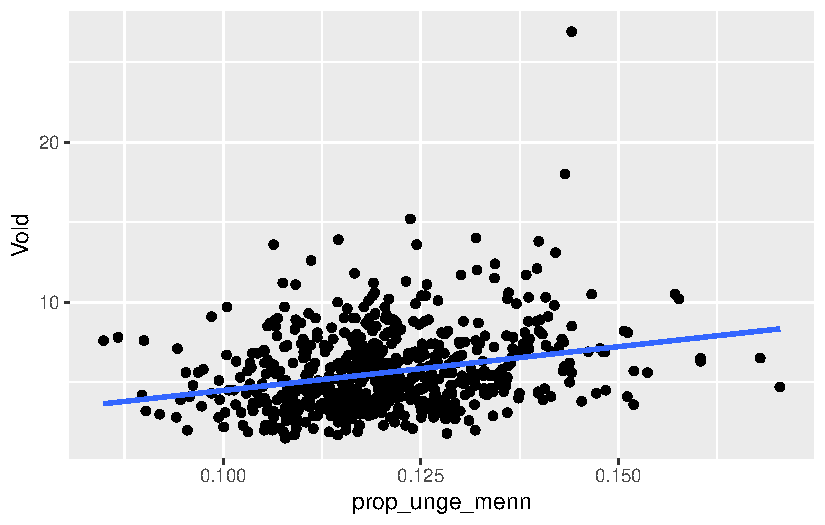
\includegraphics{./linear_regresjon_files/figure-pdf/unnamed-chunk-3-1.pdf}

}

\end{figure}

\begin{Shaded}
\begin{Highlighting}[]
\NormalTok{est }\OtherTok{\textless{}{-}} \FunctionTok{lm}\NormalTok{(Vold }\SpecialCharTok{\textasciitilde{}}\NormalTok{ prop\_unge\_menn, }\AttributeTok{data=}\NormalTok{kom\_2016)}
\FunctionTok{summary}\NormalTok{(est)}
\end{Highlighting}
\end{Shaded}

\begin{verbatim}

Call:
lm(formula = Vold ~ prop_unge_menn, data = kom_2016)

Residuals:
    Min      1Q  Median      3Q     Max 
-4.2293 -1.7014 -0.5256  1.2889 20.0062 

Coefficients:
               Estimate Std. Error t value Pr(>|t|)    
(Intercept)     -0.9949     0.9562  -1.040    0.299    
prop_unge_menn  54.7475     7.9243   6.909 1.18e-11 ***
---
Signif. codes:  0 '***' 0.001 '**' 0.01 '*' 0.05 '.' 0.1 ' ' 1

Residual standard error: 2.469 on 641 degrees of freedom
Multiple R-squared:  0.0693,    Adjusted R-squared:  0.06785 
F-statistic: 47.73 on 1 and 641 DF,  p-value: 1.181e-11
\end{verbatim}

Med andre ord kan voldsraten beskrives som

\[ vold = -0.9949 + 54.7475 \times ungeMenn  \] Men vi har også sett at
\(r^2\) er ganske lav, bare 0.0693, altså ca 7\%. Denne koeffisienten
kalles også ``coefficient of determination'' og sier noe om i hvor stor
grad modellen fanger opp variasjoenen i dataene. En lav \(r^2\) betyr at
modellen i liten grad gjør det. Vi må altså forvente at modellen vil
bomme ganske kraftig i sine prediksjoner. Vi kan velge å ta modellen
seriøst likevel, men ikke ha for store forventninger for prediksjonene!

Et annet mål på hvor godt modellen treffer er ``Root mean square
error'', RMSE. Dette kan skrives som:

\[ rmse = \sqrt{ \frac{ \sum{(O_i-P_i)^2} }{N} }  \]

der \(O\) er de observerte verdiene og \(P\) er de predikerte verdiene
for observasjon \(i\). Merk at \((O_i-P_i)\) er residualene. I R kan vi
hente ut residualene fra regresjons-objektet med dollartegnet
\texttt{...\$res} etter objektnavnet. Da kan du regne ut RMSE som
følger:

\begin{Shaded}
\begin{Highlighting}[]
\NormalTok{rmse }\OtherTok{\textless{}{-}} \FunctionTok{sqrt}\NormalTok{(}\FunctionTok{mean}\NormalTok{(est}\SpecialCharTok{$}\NormalTok{res}\SpecialCharTok{\^{}}\DecValTok{2}\NormalTok{))}
\NormalTok{rmse}
\end{Highlighting}
\end{Shaded}

\begin{verbatim}
[1] 2.465155
\end{verbatim}

RMSE sier altså omtrentlig hvor mye modellen i gjennomsnitt bommer på de
observerte verdiene. \footnote{Denne formuleringen er ganske omtrentlig.
  RMSE er egentlig kvadratroten av gjennomsnittet til de kvadrerte
  residualene, som er noe litt annet enn gjennomsnittet av de absolutte
  verdiene av residualene. Det gir bl.a. litt mer vekt til store
  residualer enn et vanlig gjennomsnitt}. Hvorvidt det er presist
\emph{nok} eller ikke vil vel strengt tatt komme an på behovet for
presisjon, altså: hva man skal bruke det til.

For å få litt bedre tak på hva RMSE betyr kan vi se på et plot av de
predikerte og observerte verdiene. Vi kan predikere vold for hver enkelt
kommune basert på denne modellen, som altså er den forventede voldsraten
\emph{hvis modellen er sann}. Funksjonen \texttt{predict()} gir oss hva
vi trenger.

\begin{Shaded}
\begin{Highlighting}[]
\NormalTok{kom }\OtherTok{\textless{}{-}}\NormalTok{ kom\_2016 }\SpecialCharTok{\%\textgreater{}\%} 
  \FunctionTok{mutate}\NormalTok{(}\AttributeTok{pred =} \FunctionTok{predict}\NormalTok{(est))}
\end{Highlighting}
\end{Shaded}

Merk at koden her lagde en kopi av datasettet der vi har alle de
opprinnelige variablene pluss en variabel med de predikerte verdiene. Vi
kan nå sammenlignet prediksjonene med de observerte utfallene.

\begin{Shaded}
\begin{Highlighting}[]
\FunctionTok{ggplot}\NormalTok{(kom, }\FunctionTok{aes}\NormalTok{(}\AttributeTok{x =}\NormalTok{ Vold, }\AttributeTok{y =}\NormalTok{ pred)) }\SpecialCharTok{+}
  \FunctionTok{geom\_point}\NormalTok{(}\AttributeTok{alpha =}\NormalTok{ .}\DecValTok{3}\NormalTok{) }\SpecialCharTok{+}
  \FunctionTok{geom\_smooth}\NormalTok{(}\AttributeTok{method =} \StringTok{"lm"}\NormalTok{, }\AttributeTok{se =} \ConstantTok{FALSE}\NormalTok{)}
\end{Highlighting}
\end{Shaded}

\begin{verbatim}
`geom_smooth()` using formula = 'y ~ x'
\end{verbatim}

\begin{figure}[H]

{\centering 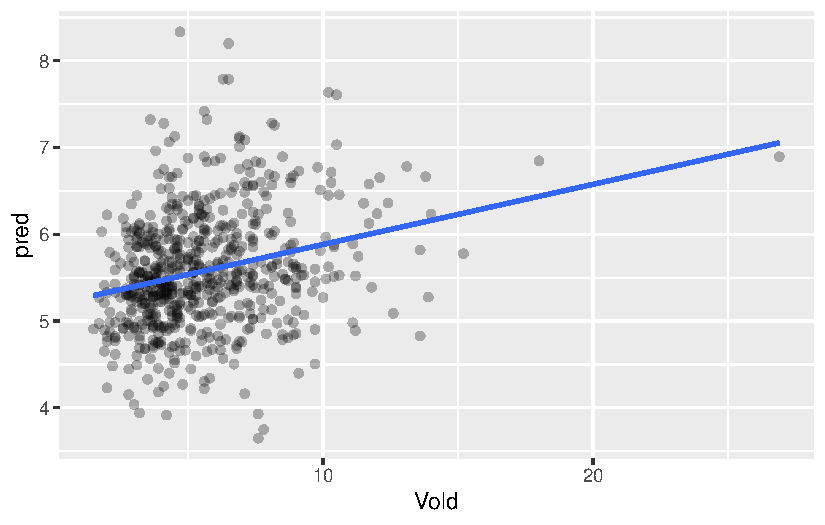
\includegraphics{./linear_regresjon_files/figure-pdf/unnamed-chunk-7-1.pdf}

}

\end{figure}

Hvis prediksjonen hadde vært perfekt ville disse punktene ligget på
linja, noe den jo ikke gjør. Modellen bommer altså ganske mye.

Hva hvis vi vil vite forventet voldsrate for en kommune for en gitt
andel unge menn? Løsningen er å lage et nytt datasett med de verdiene vi
er interessert i og så predikere for dette datasettet med å spesifisere
\texttt{newdata\ =\ dt}. Her er et eksempel der vi ønsker å vite
voldsraten hvis andelen unge menn er 15\%.

\begin{Shaded}
\begin{Highlighting}[]
\NormalTok{dt }\OtherTok{\textless{}{-}} \FunctionTok{data.frame}\NormalTok{(}\AttributeTok{prop\_unge\_menn =}\NormalTok{ .}\DecValTok{15}\NormalTok{)}
\FunctionTok{predict}\NormalTok{(est, }\AttributeTok{newdata =}\NormalTok{ dt)}
\end{Highlighting}
\end{Shaded}

\begin{verbatim}
       1 
7.217257 
\end{verbatim}

I følge modellen vil altså en kommune der 15\% av populasjonen er unge
menn ha en 7.2 voldshendelser per 1000 innbyggere. Fra tradisjonell
statistikk vet vi jo at det er usikkerhet knyttet til dette estimatet og
vi kan også ta det med i beregningen her. Vanligvis vil man estimere med
et \emph{konfidensintervall}, som gjelder hvis man estimerer et
gjennomsnitt i en gruppe. Her skal vi derimot predikere for en enkelt
kommune, som da har større usikkerhet enn om man estimerer for en enkelt
observasjon. Dette kalles prediksjonsintervall og må spesifiseres i
koden. Hvis det ikke er gitt vil R gi konfidensintervallet.

\begin{Shaded}
\begin{Highlighting}[]
\FunctionTok{predict}\NormalTok{(est, }\AttributeTok{newdata =}\NormalTok{ dt, }\AttributeTok{interval =} \StringTok{"prediction"}\NormalTok{)}
\end{Highlighting}
\end{Shaded}

\begin{verbatim}
       fit     lwr      upr
1 7.217257 2.34284 12.09167
\end{verbatim}

Tolkningen er ellers tilsvarende som for konfidensintervall: vi
forventer med ``95\% sannsynlighet''\footnote{Dette er en omtrentelig
  formulering. Alle sannsynligheter gjelder i det lange løp: altså hvis
  man gjør undersøkelsen veldig mange ganger.} at voldsraten vil være
mellom 2.3 og 12.1 per 1000 innbyggere.

\hypertarget{multippel-regresjon}{%
\subsection{Multippel regresjon}\label{multippel-regresjon}}

Enkel regresjon er nettopp enkel og prediksjonen blir ikke så god. Men
vi kan komplisere vesentlig ved å inkludere flere variable og bruke alle
triksene man evt. har lært om multippel regresjon tidligere, primært
interaksjonsledd, polynomer og transformasjoner osv.

I R vil vi da bare legge til flere variabelnavn i formelen. Ellers er
det meste likt som for enkel lineær regresjon.

\begin{Shaded}
\begin{Highlighting}[]
\NormalTok{est\_m }\OtherTok{\textless{}{-}} \FunctionTok{lm}\NormalTok{(Vold }\SpecialCharTok{\textasciitilde{}}\NormalTok{ prop\_unge\_menn }\SpecialCharTok{+}\NormalTok{ gj\_innt\_17\_34 }\SpecialCharTok{+}\NormalTok{ gj\_innt\_35\_66 }\SpecialCharTok{+} 
\NormalTok{                   prop\_shj\_mottakere\_6mnd , }
            \AttributeTok{data=}\NormalTok{kom\_2016)}
\FunctionTok{summary}\NormalTok{(est\_m)}
\end{Highlighting}
\end{Shaded}

\begin{verbatim}

Call:
lm(formula = Vold ~ prop_unge_menn + gj_innt_17_34 + gj_innt_35_66 + 
    prop_shj_mottakere_6mnd, data = kom_2016)

Residuals:
    Min      1Q  Median      3Q     Max 
-4.6397 -1.4418 -0.3125  1.2031 16.0036 

Coefficients:
                          Estimate Std. Error t value Pr(>|t|)    
(Intercept)              1.004e+00  1.115e+00   0.900    0.368    
prop_unge_menn           7.088e+01  7.337e+00   9.661  < 2e-16 ***
gj_innt_17_34           -6.220e-06  3.302e-06  -1.884    0.060 .  
gj_innt_35_66           -8.343e-06  1.651e-06  -5.053 5.68e-07 ***
prop_shj_mottakere_6mnd  2.476e+02  2.040e+01  12.134  < 2e-16 ***
---
Signif. codes:  0 '***' 0.001 '**' 0.01 '*' 0.05 '.' 0.1 ' ' 1

Residual standard error: 2.132 on 638 degrees of freedom
Multiple R-squared:  0.3091,    Adjusted R-squared:  0.3048 
F-statistic: 71.37 on 4 and 638 DF,  p-value: < 2.2e-16
\end{verbatim}

Merk at \(r^2\) nå har gått betraktelig opp, til ca 0.31. Gitt at vi
tolker dette som i hvor stor grad vi kan \emph{predikere} utfallet fra
datasettet, så er det kanskje likevel ikke imponerende høyt: vi vil
fremdeles forvente mye feil prediksjon.

Her er et scatterplot av observert mot forventet voldsrater:

\begin{Shaded}
\begin{Highlighting}[]
\NormalTok{kom\_pred }\OtherTok{\textless{}{-}}\NormalTok{ kom\_2016 }\SpecialCharTok{\%\textgreater{}\%} 
  \FunctionTok{mutate}\NormalTok{(}\AttributeTok{pred =} \FunctionTok{predict}\NormalTok{(est\_m))}

\FunctionTok{ggplot}\NormalTok{(kom\_pred, }\FunctionTok{aes}\NormalTok{(}\AttributeTok{x =}\NormalTok{ Vold, }\AttributeTok{y =}\NormalTok{ pred)) }\SpecialCharTok{+}
  \FunctionTok{geom\_point}\NormalTok{() }\SpecialCharTok{+}
  \FunctionTok{geom\_smooth}\NormalTok{(}\AttributeTok{method =} \StringTok{"lm"}\NormalTok{, }\AttributeTok{se =} \ConstantTok{FALSE}\NormalTok{)}
\end{Highlighting}
\end{Shaded}

\begin{figure}[H]

{\centering 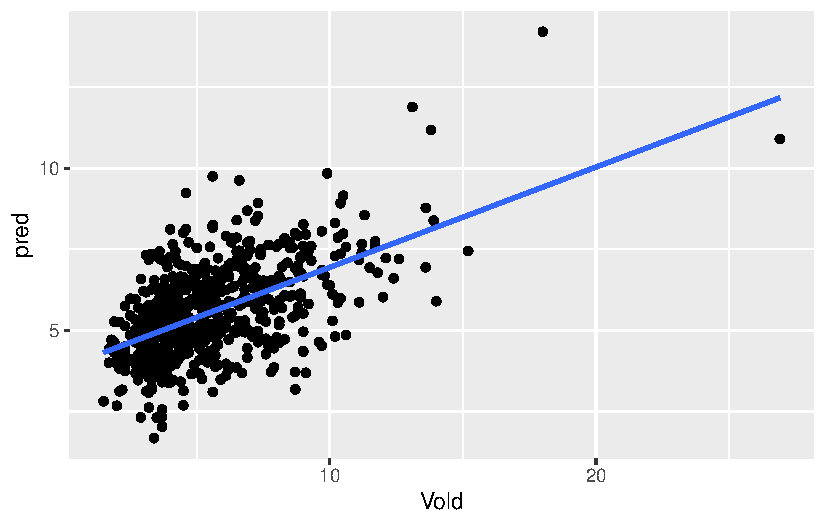
\includegraphics{./linear_regresjon_files/figure-pdf/unnamed-chunk-11-1.pdf}

}

\end{figure}

La oss inkludere alle aktuelle variable i datasettet. Et lite triks her
er å fjerne alle variable vi ikke er interessert i og lagre det i et
nytt datasett. I \texttt{lm()} kan vi da presisere formelen som
\texttt{Vold\ \textasciitilde{}\ .} som betyr å ta med alle variabelene
i stedet for å liste hver enkelt variabel.

\begin{Shaded}
\begin{Highlighting}[]
\NormalTok{kom\_s }\OtherTok{\textless{}{-}}\NormalTok{ kom\_2016 }\SpecialCharTok{\%\textgreater{}\%} 
  \FunctionTok{select}\NormalTok{(}\SpecialCharTok{{-}}\FunctionTok{c}\NormalTok{(kommune, lovb\_ialt, Orden,  }
\NormalTok{            Rusmiddellovbrudd, Trafikkovertredelse, }
\NormalTok{            lovb\_annet, prop\_unge\_menn))}

\NormalTok{full\_mod }\OtherTok{\textless{}{-}} \FunctionTok{lm}\NormalTok{(Vold }\SpecialCharTok{\textasciitilde{}}\NormalTok{ . , }\AttributeTok{data =}\NormalTok{ kom\_s)}
\FunctionTok{summary}\NormalTok{(full\_mod)}
\end{Highlighting}
\end{Shaded}

\begin{verbatim}

Call:
lm(formula = Vold ~ ., data = kom_s)

Residuals:
    Min      1Q  Median      3Q     Max 
-5.2272 -1.3129 -0.2606  1.1059 13.8145 

Coefficients:
                          Estimate Std. Error t value Pr(>|t|)    
(Intercept)              1.714e+00  3.228e+02   0.005  0.99577    
year                    -9.970e-04  1.602e-01  -0.006  0.99504    
bef_tot                  4.440e-06  2.276e-06   1.951  0.05154 .  
prop_kvinner_16_18      -7.445e+01  3.803e+01  -1.958  0.05069 .  
prop_menn_16_18          1.529e+01  3.066e+01   0.499  0.61829    
prop_menn_19_34          6.935e+01  1.176e+01   5.897 6.03e-09 ***
prop_kvinner_19_34       2.019e+00  1.278e+01   0.158  0.87447    
prop_shj_mottakere       1.010e+02  1.463e+01   6.899 1.28e-11 ***
prop_shj_mottakere_6mnd  5.294e+01  3.102e+01   1.707  0.08837 .  
gj_innt_17_34           -1.359e-05  4.226e-06  -3.217  0.00136 ** 
gj_innt_35_66           -2.058e-05  8.411e-06  -2.447  0.01468 *  
gj_innt_alle             2.665e-05  1.224e-05   2.177  0.02987 *  
---
Signif. codes:  0 '***' 0.001 '**' 0.01 '*' 0.05 '.' 0.1 ' ' 1

Residual standard error: 2.018 on 631 degrees of freedom
Multiple R-squared:  0.3878,    Adjusted R-squared:  0.3772 
F-statistic: 36.34 on 11 and 631 DF,  p-value: < 2.2e-16
\end{verbatim}

\(r^2\) gikk noe opp, til 0.39.

Men vi kan gjøre modellen ekstra komplisert ved inkludere alle mulige
interaksjonsledd. En åpenbar ulempe med dette er at hver enkelt
koeffisent blir svært mye vanskeligere å tolke. Vi fokuserer derfor kun
på \(r^2\) som kan hentes ut uten å ta med resten av output.

\begin{Shaded}
\begin{Highlighting}[]
\NormalTok{full\_mod2 }\OtherTok{\textless{}{-}} \FunctionTok{lm}\NormalTok{( Vold }\SpecialCharTok{\textasciitilde{}}\NormalTok{ .}\SpecialCharTok{\^{}}\DecValTok{2}\NormalTok{, }\AttributeTok{data =}\NormalTok{ kom\_s)}
\FunctionTok{summary}\NormalTok{(full\_mod2)}\SpecialCharTok{$}\NormalTok{r.squared}
\end{Highlighting}
\end{Shaded}

\begin{verbatim}
[1] 0.529478
\end{verbatim}

\(r^2\) gikk vesentlig opp. Men når vi først driver med kompliserte
modellspesifikasjoner som uansett er vanskelige å tolke - hvorfor
begrense seg til 2-veis interaksjoner? Her er en versjon med alle 3-veis
interaksjoner, og nå begynner \(r^2\) virkelig å bli høy!

\begin{Shaded}
\begin{Highlighting}[]
\NormalTok{full\_mod3 }\OtherTok{\textless{}{-}} \FunctionTok{lm}\NormalTok{( Vold }\SpecialCharTok{\textasciitilde{}}\NormalTok{ .}\SpecialCharTok{\^{}}\DecValTok{3}\NormalTok{, }\AttributeTok{data =}\NormalTok{ kom\_s)}
\FunctionTok{summary}\NormalTok{(full\_mod3)}\SpecialCharTok{$}\NormalTok{r.squared}
\end{Highlighting}
\end{Shaded}

\begin{verbatim}
[1] 0.7215881
\end{verbatim}

Vi kan trimme modellen så den ikke har med så voldsomt mange parametre.
En mulighet er å overlate dette til datamaskinen ved å la den gjøre en
trinnvis test av hvorvidt modellene blir signifikant dårligere av å ta
vekk noen ledd. Så beholdes den ``beste'' modellen.

OBS! Merk at dette er en rent mekanisk seleksjon, og frarådes i de
fleste samfunnsvitenskapelige sammenhenger. Tolkning av parametre og
statistisk usikkerhet er nå på svært tynn is. Men det kan gi god
prediksjon likevel.

\begin{Shaded}
\begin{Highlighting}[]
\NormalTok{step\_mod }\OtherTok{\textless{}{-}}\NormalTok{ MASS}\SpecialCharTok{::}\FunctionTok{stepAIC}\NormalTok{(full\_mod3, }\AttributeTok{direction=}\StringTok{"backward"}\NormalTok{, }
                          \AttributeTok{trace =} \ConstantTok{FALSE}\NormalTok{)}
\FunctionTok{summary}\NormalTok{(step\_mod)}\SpecialCharTok{$}\NormalTok{r.squared}
\end{Highlighting}
\end{Shaded}

\begin{verbatim}
[1] 0.7046848
\end{verbatim}

Hvis vi nå predikerer for hver enkelt kommune og plotter forventet mot
observert, så får vi et svært mye bedre sammenfall enn tidligere.

\begin{Shaded}
\begin{Highlighting}[]
\NormalTok{kom\_pred }\OtherTok{\textless{}{-}}\NormalTok{ kom\_s }\SpecialCharTok{\%\textgreater{}\%} 
  \FunctionTok{mutate}\NormalTok{(}\AttributeTok{pred =} \FunctionTok{predict}\NormalTok{(step\_mod))}

\FunctionTok{ggplot}\NormalTok{(kom\_pred, }\FunctionTok{aes}\NormalTok{(}\AttributeTok{x =}\NormalTok{ Vold, }\AttributeTok{y =}\NormalTok{ pred)) }\SpecialCharTok{+}
  \FunctionTok{geom\_point}\NormalTok{(}\AttributeTok{alpha =}\NormalTok{ .}\DecValTok{3}\NormalTok{) }\SpecialCharTok{+}
  \FunctionTok{geom\_smooth}\NormalTok{(}\AttributeTok{method =} \StringTok{"lm"}\NormalTok{, }\AttributeTok{se =} \ConstantTok{FALSE}\NormalTok{)}
\end{Highlighting}
\end{Shaded}

\begin{figure}[H]

{\centering 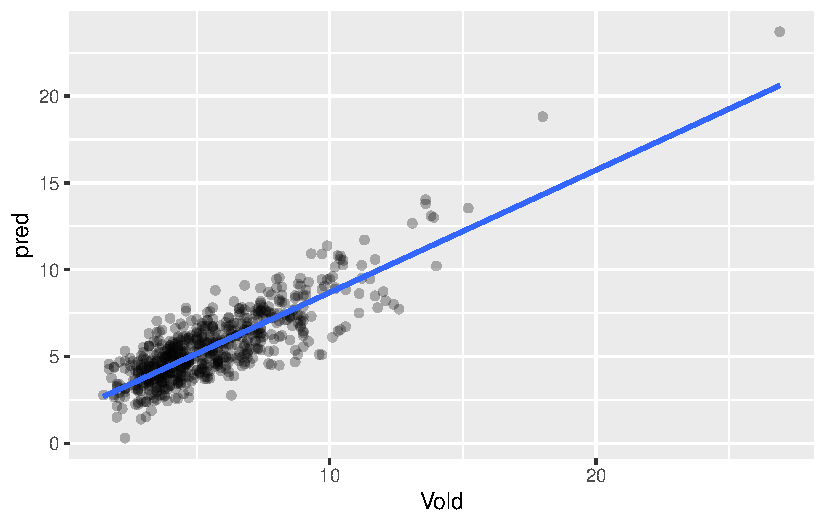
\includegraphics{./linear_regresjon_files/figure-pdf/unnamed-chunk-15-1.pdf}

}

\end{figure}

Nå kan vi også regne ut RMSE, som altså er ``root mean squared error''.
Med andre ord: regn ut residualene (dvs. ``error''), og kvadrer denne,
og så ta kvadratroten av gjennomsnittet av denne. Her er en kode skrevet
litt omstendelig så den er litt lettere å forstå:

\begin{Shaded}
\begin{Highlighting}[]
\NormalTok{kom\_s }\SpecialCharTok{\%\textgreater{}\%} 
  \FunctionTok{mutate}\NormalTok{(}\AttributeTok{pred =} \FunctionTok{predict}\NormalTok{(step\_mod), }
         \AttributeTok{residual =}\NormalTok{ pred }\SpecialCharTok{{-}}\NormalTok{ Vold) }\SpecialCharTok{\%\textgreater{}\%} 
  \FunctionTok{mutate}\NormalTok{(}\AttributeTok{sq.resid =}\NormalTok{ residual}\SpecialCharTok{\^{}}\DecValTok{2}\NormalTok{) }\SpecialCharTok{\%\textgreater{}\%} 
  \FunctionTok{summarise}\NormalTok{(}\FunctionTok{sqrt}\NormalTok{(}\FunctionTok{mean}\NormalTok{(sq.resid)))}
\end{Highlighting}
\end{Shaded}

\begin{verbatim}
  sqrt(mean(sq.resid))
1              1.38862
\end{verbatim}

Dette betyr omtrentlig at modellen i gjennomsnitt vil bomme med 1.38
prosentpoeng på voldsraten i kommunen. \footnote{Denne formuleringen er
  ganske omtrentlig. RMSE er egentlig kvadratroten av gjennomsnittet til
  de kvadrerte residualene, som er noe litt annet enn gjennomsnittet av
  de absolutte verdiene av residualene. Det gir bl.a. litt mer vekt til
  store residualer enn et vanlig gjennomsnitt}. Hvorvidt det er presist
\emph{nok} eller ikke vil vel strengt tatt komme an på behovet for
presisjon, altså: hva man skal bruke det til.

\hypertarget{oppgaver-1}{%
\section{Oppgaver}\label{oppgaver-1}}

\leavevmode\vadjust pre{\hypertarget{exr-ols-eksplisitt}{}}%
\begin{exercise}[]\label{exr-ols-eksplisitt}

Velg et datasettet og formuler hva en prediksjonsmodell kan kunne brukes
til. Se for deg at tiltak du foreslår vil altså ha faktiske
konsekvenser, så gjør en vurdering av hvorvidt feilprediksjoner vil være
problematiske og i så fall på hvilken måte. Vurder mulighetene for feil
opp mot gevinst ved riktig prediksjon.

Merk: det er ikke viktig at anvendelsen skal være realistisk, men du må
alltid ta konsekvensen i vurderingene.

\end{exercise}

\leavevmode\vadjust pre{\hypertarget{exr-split}{}}%
\begin{exercise}[]\label{exr-split}

Last inn valgte datasett og splitt i et training og et testing datasett.
Sett splitten ved .70. Bruk training-data til å gjøre deg kjent med
dataene og estimere modellene. Ikke bruk testing-dataene inntil du får
beskjed om det.

\end{exercise}

\leavevmode\vadjust pre{\hypertarget{exr-sepaa}{}}%
\begin{exercise}[]\label{exr-sepaa}

Gjør deg kjent med innholdet i disse training-dataene. Du kan gjøre
f.eks. følgende:

\begin{enumerate}
\def\labelenumi{\alph{enumi})}
\tightlist
\item
  Bruk \texttt{glimpse()} og \texttt{skim()} til å få oversikt over
  innholdet i datasettet
\item
  Hvis det er noen variable du ikke kommer til å bruke, slett gjerne
  disse med en gang
\item
  Lag noen tabeller og plot som viser hvordan utfallsvariabelen er
  fordelt etter andre variable
\end{enumerate}

\end{exercise}

\leavevmode\vadjust pre{\hypertarget{exr-ols-train}{}}%
\begin{exercise}[]\label{exr-ols-train}

Estimer flere lineær regresjonsmodeller med et fåtall prediktorer. Gjør
et utvalg av de variablene du mener er mest relevant for å forklare
utfallet. Estimer flere lineære regresjonsmodeller for å predikere
utfallet, og sammenlign hvor gode prediksjoner disse gir. Mest relevante
statistikker er \(r^2\) og RMSE.

\begin{enumerate}
\def\labelenumi{\alph{enumi})}
\tightlist
\item
  Velg ut tre forklaringsvariable og estimer en regresjonsmodell
\item
  Estimer en ny modell med alle variable i datasettet
\item
  Estimer en ny modell og inkluder noen få polynomer og/eller
  interaksjonsledd
\item
  Gjør et automatisk modellsøk
\end{enumerate}

Lag gjerne noen plot av ROC-curve for i hvert fall noen av modellene
slik at du får en følelse med hva AUC egentlig betyr. Plot også
predikert verdi mot observert verdi og gjør en vurdering av RMSE.

\end{exercise}

\leavevmode\vadjust pre{\hypertarget{exr-ols-test}{}}%
\begin{exercise}[]\label{exr-ols-test}

I forrige oppgave brukte du testing-datasettet til både å estimere
modellene og vurdere resultatet. Nå skal du bruke testing-datasettet til
å vurdere de samme resultatene. Dette gjør du ved å predikere på
testing-datasettet og regne ut AUC og RMSE for disse dataene. For hver
modell i forrige oppgave, gjør som følger:

\begin{enumerate}
\def\labelenumi{\alph{enumi})}
\tightlist
\item
  Prediker utfallet på testing-datasettet
\item
  Regn ut AUC og RMSE
\item
  Hvor stor er \emph{endringen} i AUC og RMSE fra resultatene når du
  brukte training-datasettet?
\end{enumerate}

Vurdering: En mer komplisert modell beskriver dataene bedre. Men er det
like stor \emph{endring} i AUC og RMSE for enkle og mer kompliserte
modeller? Beskriv hva du ser og gi en forklaring.

\end{exercise}

\bookmarksetup{startatroot}

\hypertarget{logistisk-regresjon}{%
\chapter{Logistisk regresjon}\label{logistisk-regresjon}}

\hypertarget{logistisk-regresjon-i-r}{%
\section{Logistisk regresjon i R}\label{logistisk-regresjon-i-r}}

Logistisk regresjon har det til felles med lineær regresjon at utfallet
er en lineær spesifikasjon.

\[  log( \frac{\pi}{(1-\pi)}) = \alpha + \beta X \]

Venstresiden av ligningen kalles en \emph{logit}, der \(\pi\) er en
sannsynlighet. Uttrykket \(\frac{\pi}{(1-\pi)}\) er en \emph{odds}, som
er et forholdstall mellom sannsynligheten for at utfallet skjer mot
sannsynligheten for det motsatte. Tolkningen av \(\beta\) er da en
endring av \emph{odds} på logaritisk skala. Hvis man eksponensierer
\(\beta\) er den da tolkbar som en \emph{oddsrate}.

Som du nå sikkert skjønner så er altså tolkningen av
regresjonskoeffisientene nokså krøkete å tolke substansielt for de
fleste av oss. Det kan i seg selv være et argument mot å bruke logistisk
regresjon i en del sammenhenger.

Men man kan regne om til sannsynligheter som er vesentlig enklere å
forstå. Særlig hvis man ikke er så interessert i tolkningen av
\(\beta\), men prediksjon av \(\pi\).

Ligningen kan da skrives om slik at venstresiden av ligningen blir en
sannsynlighet direkte:

\[  \pi = \frac{e^{\alpha + \beta X}}{1 + e^{\alpha + \beta X}} \]

En enkel omregning av regresjonsresultatet gir altså en
\emph{sannynlighet}. Denne sannsynligheten kan vi da bruke til
\emph{klassifikasjon} hvis det er formålet med analysen. Hvis
utfallsvariabelen har to kategorier, så er en nærliggende mulighet å
klassifisere til den gruppen hver person mest sannsynlig tilhører.
Altså: de som har \(P(y = 1) > 0.5\) tilhører den ene gruppen og resten
i den andre gruppen.

\hypertarget{empirisk-eksempel}{%
\section{Empirisk eksempel}\label{empirisk-eksempel}}

Som eksempel bruker vi et datasettet Attrition. Dette er et datasett
over arbeidstakere i en bedrift der utfallsvariabelen er om
arbeidstakeren slutter i jobben eller ikke.

For arbeidsgivere kan det være kostbart med endringer i staben.
Arbeidstakere som slutter tar med seg erfaring og kompetanse, og nye
arbeidstakere må læres opp. Arbeidsgiver bør derfor generelt legge til
rette for at arbeidstakere ønsker å bli værende, men det kan også være
aktuelt med mer målrettede tiltak. Når en arbeidstaker har fått et nytt
jobbtilbud kan det være for sent. Hvis man derimot kan komme i forkjøpet
kan man kanskje gjøre noe \emph{før} vedkommende går til det skrittet å
søke ny jobb. Hvis man kunne predikere hvem som kommer til å slutte
kunne man altså gjort tiltak i forkant.\footnote{Her kunne man jo også
  tenke seg at den gode lederen har en dialog med de ansatte og fanger
  opp deres frustrasjoner og behov slik at maskinell prediksjon ikke
  trengs. Det er jo også en form for prediksjon med kvalitative data! Så
  her er vi i en setting der dette ikke fungerer eller det er så store
  forhold at en kvalitativ tilnærming ikke er praktisk mulig eller noe
  sånt.}

Først leser vi inn datasettet og evt. laster pakker i trenger. Dataene
er i csv-format så vi leser inn med \texttt{read.csv()}. Deretter kan vi
se på innholdet med \texttt{skim()}:

\begin{Shaded}
\begin{Highlighting}[]
\FunctionTok{library}\NormalTok{(tidyverse) }
\FunctionTok{library}\NormalTok{(pROC) }
\FunctionTok{library}\NormalTok{(skimr)}
\NormalTok{attrition }\OtherTok{\textless{}{-}}\FunctionTok{read.csv}\NormalTok{(}\StringTok{"../data/Attrition.csv"}\NormalTok{, }\AttributeTok{stringsAsFactors =} \ConstantTok{TRUE}\NormalTok{)  }
\FunctionTok{skim}\NormalTok{(attrition)  }
\end{Highlighting}
\end{Shaded}

\begin{longtable}[]{@{}ll@{}}
\caption{Data summary}\tabularnewline
\toprule()
\endhead
Name & attrition \\
Number of rows & 1470 \\
Number of columns & 36 \\
\_\_\_\_\_\_\_\_\_\_\_\_\_\_\_\_\_\_\_\_\_\_\_ & \\
Column type frequency: & \\
factor & 9 \\
numeric & 27 \\
\_\_\_\_\_\_\_\_\_\_\_\_\_\_\_\_\_\_\_\_\_\_\_\_ & \\
Group variables & None \\
\bottomrule()
\end{longtable}

\textbf{Variable type: factor}

\begin{longtable}[]{@{}
  >{\raggedright\arraybackslash}p{(\columnwidth - 10\tabcolsep) * \real{0.1579}}
  >{\raggedleft\arraybackslash}p{(\columnwidth - 10\tabcolsep) * \real{0.1053}}
  >{\raggedleft\arraybackslash}p{(\columnwidth - 10\tabcolsep) * \real{0.1474}}
  >{\raggedright\arraybackslash}p{(\columnwidth - 10\tabcolsep) * \real{0.0842}}
  >{\raggedleft\arraybackslash}p{(\columnwidth - 10\tabcolsep) * \real{0.0947}}
  >{\raggedright\arraybackslash}p{(\columnwidth - 10\tabcolsep) * \real{0.4105}}@{}}
\toprule()
\begin{minipage}[b]{\linewidth}\raggedright
skim\_variable
\end{minipage} & \begin{minipage}[b]{\linewidth}\raggedleft
n\_missing
\end{minipage} & \begin{minipage}[b]{\linewidth}\raggedleft
complete\_rate
\end{minipage} & \begin{minipage}[b]{\linewidth}\raggedright
ordered
\end{minipage} & \begin{minipage}[b]{\linewidth}\raggedleft
n\_unique
\end{minipage} & \begin{minipage}[b]{\linewidth}\raggedright
top\_counts
\end{minipage} \\
\midrule()
\endhead
Attrition & 0 & 1 & FALSE & 2 & No: 1233, Yes: 237 \\
BusinessTravel & 0 & 1 & FALSE & 3 & Tra: 1043, Tra: 277, Non: 150 \\
Department & 0 & 1 & FALSE & 3 & Res: 961, Sal: 446, Hum: 63 \\
EducationField & 0 & 1 & FALSE & 6 & Lif: 606, Med: 464, Mar: 159, Tec:
132 \\
Gender & 0 & 1 & FALSE & 2 & Mal: 882, Fem: 588 \\
JobRole & 0 & 1 & FALSE & 9 & Sal: 326, Res: 292, Lab: 259, Man: 145 \\
MaritalStatus & 0 & 1 & FALSE & 3 & Mar: 673, Sin: 470, Div: 327 \\
Over18 & 0 & 1 & FALSE & 1 & Y: 1470 \\
OverTime & 0 & 1 & FALSE & 2 & No: 1054, Yes: 416 \\
\bottomrule()
\end{longtable}

\textbf{Variable type: numeric}

\begin{longtable}[]{@{}
  >{\raggedright\arraybackslash}p{(\columnwidth - 20\tabcolsep) * \real{0.2315}}
  >{\raggedleft\arraybackslash}p{(\columnwidth - 20\tabcolsep) * \real{0.0926}}
  >{\raggedleft\arraybackslash}p{(\columnwidth - 20\tabcolsep) * \real{0.1296}}
  >{\raggedleft\arraybackslash}p{(\columnwidth - 20\tabcolsep) * \real{0.0833}}
  >{\raggedleft\arraybackslash}p{(\columnwidth - 20\tabcolsep) * \real{0.0741}}
  >{\raggedleft\arraybackslash}p{(\columnwidth - 20\tabcolsep) * \real{0.0463}}
  >{\raggedleft\arraybackslash}p{(\columnwidth - 20\tabcolsep) * \real{0.0741}}
  >{\raggedleft\arraybackslash}p{(\columnwidth - 20\tabcolsep) * \real{0.0741}}
  >{\raggedleft\arraybackslash}p{(\columnwidth - 20\tabcolsep) * \real{0.0833}}
  >{\raggedleft\arraybackslash}p{(\columnwidth - 20\tabcolsep) * \real{0.0556}}
  >{\raggedright\arraybackslash}p{(\columnwidth - 20\tabcolsep) * \real{0.0556}}@{}}
\toprule()
\begin{minipage}[b]{\linewidth}\raggedright
skim\_variable
\end{minipage} & \begin{minipage}[b]{\linewidth}\raggedleft
n\_missing
\end{minipage} & \begin{minipage}[b]{\linewidth}\raggedleft
complete\_rate
\end{minipage} & \begin{minipage}[b]{\linewidth}\raggedleft
mean
\end{minipage} & \begin{minipage}[b]{\linewidth}\raggedleft
sd
\end{minipage} & \begin{minipage}[b]{\linewidth}\raggedleft
p0
\end{minipage} & \begin{minipage}[b]{\linewidth}\raggedleft
p25
\end{minipage} & \begin{minipage}[b]{\linewidth}\raggedleft
p50
\end{minipage} & \begin{minipage}[b]{\linewidth}\raggedleft
p75
\end{minipage} & \begin{minipage}[b]{\linewidth}\raggedleft
p100
\end{minipage} & \begin{minipage}[b]{\linewidth}\raggedright
hist
\end{minipage} \\
\midrule()
\endhead
X & 0 & 1 & 735.50 & 424.50 & 1 & 368.25 & 735.5 & 1102.75 & 1470 &
▇▇▇▇▇ \\
Age & 0 & 1 & 36.92 & 9.14 & 18 & 30.00 & 36.0 & 43.00 & 60 & ▂▇▇▃▂ \\
DailyRate & 0 & 1 & 802.49 & 403.51 & 102 & 465.00 & 802.0 & 1157.00 &
1499 & ▇▇▇▇▇ \\
DistanceFromHome & 0 & 1 & 9.19 & 8.11 & 1 & 2.00 & 7.0 & 14.00 & 29 &
▇▅▂▂▂ \\
Education & 0 & 1 & 2.91 & 1.02 & 1 & 2.00 & 3.0 & 4.00 & 5 & ▂▃▇▆▁ \\
EmployeeCount & 0 & 1 & 1.00 & 0.00 & 1 & 1.00 & 1.0 & 1.00 & 1 &
▁▁▇▁▁ \\
EmployeeNumber & 0 & 1 & 1024.87 & 602.02 & 1 & 491.25 & 1020.5 &
1555.75 & 2068 & ▇▇▇▇▇ \\
EnvironmentSatisfaction & 0 & 1 & 2.72 & 1.09 & 1 & 2.00 & 3.0 & 4.00 &
4 & ▅▅▁▇▇ \\
HourlyRate & 0 & 1 & 65.89 & 20.33 & 30 & 48.00 & 66.0 & 83.75 & 100 &
▇▇▇▇▇ \\
JobInvolvement & 0 & 1 & 2.73 & 0.71 & 1 & 2.00 & 3.0 & 3.00 & 4 &
▁▃▁▇▁ \\
JobLevel & 0 & 1 & 2.06 & 1.11 & 1 & 1.00 & 2.0 & 3.00 & 5 & ▇▇▃▂▁ \\
JobSatisfaction & 0 & 1 & 2.73 & 1.10 & 1 & 2.00 & 3.0 & 4.00 & 4 &
▅▅▁▇▇ \\
MonthlyIncome & 0 & 1 & 6502.93 & 4707.96 & 1009 & 2911.00 & 4919.0 &
8379.00 & 19999 & ▇▅▂▁▂ \\
MonthlyRate & 0 & 1 & 14313.10 & 7117.79 & 2094 & 8047.00 & 14235.5 &
20461.50 & 26999 & ▇▇▇▇▇ \\
NumCompaniesWorked & 0 & 1 & 2.69 & 2.50 & 0 & 1.00 & 2.0 & 4.00 & 9 &
▇▃▂▂▁ \\
PercentSalaryHike & 0 & 1 & 15.21 & 3.66 & 11 & 12.00 & 14.0 & 18.00 &
25 & ▇▅▃▂▁ \\
PerformanceRating & 0 & 1 & 3.15 & 0.36 & 3 & 3.00 & 3.0 & 3.00 & 4 &
▇▁▁▁▂ \\
RelationshipSatisfaction & 0 & 1 & 2.71 & 1.08 & 1 & 2.00 & 3.0 & 4.00 &
4 & ▅▅▁▇▇ \\
StandardHours & 0 & 1 & 80.00 & 0.00 & 80 & 80.00 & 80.0 & 80.00 & 80 &
▁▁▇▁▁ \\
StockOptionLevel & 0 & 1 & 0.79 & 0.85 & 0 & 0.00 & 1.0 & 1.00 & 3 &
▇▇▁▂▁ \\
TotalWorkingYears & 0 & 1 & 11.28 & 7.78 & 0 & 6.00 & 10.0 & 15.00 & 40
& ▇▇▂▁▁ \\
TrainingTimesLastYear & 0 & 1 & 2.80 & 1.29 & 0 & 2.00 & 3.0 & 3.00 & 6
& ▂▇▇▂▃ \\
WorkLifeBalance & 0 & 1 & 2.76 & 0.71 & 1 & 2.00 & 3.0 & 3.00 & 4 &
▁▃▁▇▂ \\
YearsAtCompany & 0 & 1 & 7.01 & 6.13 & 0 & 3.00 & 5.0 & 9.00 & 40 &
▇▂▁▁▁ \\
YearsInCurrentRole & 0 & 1 & 4.23 & 3.62 & 0 & 2.00 & 3.0 & 7.00 & 18 &
▇▃▂▁▁ \\
YearsSinceLastPromotion & 0 & 1 & 2.19 & 3.22 & 0 & 0.00 & 1.0 & 3.00 &
15 & ▇▁▁▁▁ \\
YearsWithCurrManager & 0 & 1 & 4.12 & 3.57 & 0 & 2.00 & 3.0 & 7.00 & 17
& ▇▂▅▁▁ \\
\bottomrule()
\end{longtable}

Merk at det er fire variable vi ikke trenger, så vi sletter disse like
gjerne med en gang:

\begin{itemize}
\tightlist
\item
  x er et løpenummer.
\item
  Over18 er en dummy for om de er over 18 år. Det er alle.
\item
  EmployeeCount og StandardHours varierer heller ikke.
\end{itemize}

Bruker select() med minustegn for variable vi vil fjerne. Her
overskrives datasettet med det modifiserte datasettet

\begin{Shaded}
\begin{Highlighting}[]
\NormalTok{attrition }\OtherTok{\textless{}{-}}\NormalTok{ attrition }\SpecialCharTok{\%\textgreater{}\%}  
  \FunctionTok{select}\NormalTok{(}\SpecialCharTok{{-}}\NormalTok{X, }\SpecialCharTok{{-}}\NormalTok{ Over18, }\SpecialCharTok{{-}}\NormalTok{ EmployeeCount, }\SpecialCharTok{{-}}\NormalTok{StandardHours) }
\FunctionTok{glimpse}\NormalTok{(attrition)}
\end{Highlighting}
\end{Shaded}

\begin{verbatim}
Rows: 1,470
Columns: 32
$ Age                      <int> 41, 49, 37, 33, 27, 32, 59, 30, 38, 36, 35, 2~
$ Attrition                <fct> Yes, No, Yes, No, No, No, No, No, No, No, No,~
$ BusinessTravel           <fct> Travel_Rarely, Travel_Frequently, Travel_Rare~
$ DailyRate                <int> 1102, 279, 1373, 1392, 591, 1005, 1324, 1358,~
$ Department               <fct> Sales, Research & Development, Research & Dev~
$ DistanceFromHome         <int> 1, 8, 2, 3, 2, 2, 3, 24, 23, 27, 16, 15, 26, ~
$ Education                <int> 2, 1, 2, 4, 1, 2, 3, 1, 3, 3, 3, 2, 1, 2, 3, ~
$ EducationField           <fct> Life Sciences, Life Sciences, Other, Life Sci~
$ EmployeeNumber           <int> 1, 2, 4, 5, 7, 8, 10, 11, 12, 13, 14, 15, 16,~
$ EnvironmentSatisfaction  <int> 2, 3, 4, 4, 1, 4, 3, 4, 4, 3, 1, 4, 1, 2, 3, ~
$ Gender                   <fct> Female, Male, Male, Female, Male, Male, Femal~
$ HourlyRate               <int> 94, 61, 92, 56, 40, 79, 81, 67, 44, 94, 84, 4~
$ JobInvolvement           <int> 3, 2, 2, 3, 3, 3, 4, 3, 2, 3, 4, 2, 3, 3, 2, ~
$ JobLevel                 <int> 2, 2, 1, 1, 1, 1, 1, 1, 3, 2, 1, 2, 1, 1, 1, ~
$ JobRole                  <fct> Sales Executive, Research Scientist, Laborato~
$ JobSatisfaction          <int> 4, 2, 3, 3, 2, 4, 1, 3, 3, 3, 2, 3, 3, 4, 3, ~
$ MaritalStatus            <fct> Single, Married, Single, Married, Married, Si~
$ MonthlyIncome            <int> 5993, 5130, 2090, 2909, 3468, 3068, 2670, 269~
$ MonthlyRate              <int> 19479, 24907, 2396, 23159, 16632, 11864, 9964~
$ NumCompaniesWorked       <int> 8, 1, 6, 1, 9, 0, 4, 1, 0, 6, 0, 0, 1, 0, 5, ~
$ OverTime                 <fct> Yes, No, Yes, Yes, No, No, Yes, No, No, No, N~
$ PercentSalaryHike        <int> 11, 23, 15, 11, 12, 13, 20, 22, 21, 13, 13, 1~
$ PerformanceRating        <int> 3, 4, 3, 3, 3, 3, 4, 4, 4, 3, 3, 3, 3, 3, 3, ~
$ RelationshipSatisfaction <int> 1, 4, 2, 3, 4, 3, 1, 2, 2, 2, 3, 4, 4, 3, 2, ~
$ StockOptionLevel         <int> 0, 1, 0, 0, 1, 0, 3, 1, 0, 2, 1, 0, 1, 1, 0, ~
$ TotalWorkingYears        <int> 8, 10, 7, 8, 6, 8, 12, 1, 10, 17, 6, 10, 5, 3~
$ TrainingTimesLastYear    <int> 0, 3, 3, 3, 3, 2, 3, 2, 2, 3, 5, 3, 1, 2, 4, ~
$ WorkLifeBalance          <int> 1, 3, 3, 3, 3, 2, 2, 3, 3, 2, 3, 3, 2, 3, 3, ~
$ YearsAtCompany           <int> 6, 10, 0, 8, 2, 7, 1, 1, 9, 7, 5, 9, 5, 2, 4,~
$ YearsInCurrentRole       <int> 4, 7, 0, 7, 2, 7, 0, 0, 7, 7, 4, 5, 2, 2, 2, ~
$ YearsSinceLastPromotion  <int> 0, 1, 0, 3, 2, 3, 0, 0, 1, 7, 0, 0, 4, 1, 0, ~
$ YearsWithCurrManager     <int> 5, 7, 0, 0, 2, 6, 0, 0, 8, 7, 3, 8, 3, 2, 3, ~
\end{verbatim}

Del datasettet i to deler. Vi trekker tilfeldig 70\% og legger dette i
datasettet training. Resten legges i testing.

Lager først en rekke tilfeldige tall mellom 0 og 1 med samme lengde som
datasettet:

\begin{Shaded}
\begin{Highlighting}[]
\NormalTok{lottery }\OtherTok{\textless{}{-}} \FunctionTok{runif}\NormalTok{(}\AttributeTok{n =} \FunctionTok{nrow}\NormalTok{(attrition))  }
\end{Highlighting}
\end{Shaded}

Datasettet deles etter hvilke rader som tilsvarer tilfeldig tall under
og over .7

\begin{Shaded}
\begin{Highlighting}[]
\NormalTok{grense }\OtherTok{\textless{}{-}} \FloatTok{0.7} 
\NormalTok{training }\OtherTok{\textless{}{-}} \FunctionTok{filter}\NormalTok{(attrition, lottery }\SpecialCharTok{\textless{}}\NormalTok{ grense) }
\NormalTok{testing  }\OtherTok{\textless{}{-}} \FunctionTok{filter}\NormalTok{(attrition, lottery }\SpecialCharTok{\textgreater{}=}\NormalTok{ grense) }
\end{Highlighting}
\end{Shaded}

Sjekk at antallet i hvert datasett summeres til totalen

\begin{Shaded}
\begin{Highlighting}[]
\FunctionTok{nrow}\NormalTok{(attrition) }
\end{Highlighting}
\end{Shaded}

\begin{verbatim}
[1] 1470
\end{verbatim}

\begin{Shaded}
\begin{Highlighting}[]
\FunctionTok{nrow}\NormalTok{(training) }
\end{Highlighting}
\end{Shaded}

\begin{verbatim}
[1] 1024
\end{verbatim}

\begin{Shaded}
\begin{Highlighting}[]
\FunctionTok{nrow}\NormalTok{(testing) }
\end{Highlighting}
\end{Shaded}

\begin{verbatim}
[1] 446
\end{verbatim}

OBS! variabelen Attrition er en ``factor'', dvs. kategorisk med
underliggende nummer. Ta en titt.

\begin{Shaded}
\begin{Highlighting}[]
\FunctionTok{str}\NormalTok{(training}\SpecialCharTok{$}\NormalTok{Attrition)   }
\end{Highlighting}
\end{Shaded}

\begin{verbatim}
 Factor w/ 2 levels "No","Yes": 2 1 2 1 1 1 1 1 1 1 ...
\end{verbatim}

\begin{Shaded}
\begin{Highlighting}[]
\FunctionTok{head}\NormalTok{(training}\SpecialCharTok{$}\NormalTok{Attrition) }
\end{Highlighting}
\end{Shaded}

\begin{verbatim}
[1] Yes No  Yes No  No  No 
Levels: No Yes
\end{verbatim}

\begin{Shaded}
\begin{Highlighting}[]
\FunctionTok{levels}\NormalTok{(training}\SpecialCharTok{$}\NormalTok{Attrition) }
\end{Highlighting}
\end{Shaded}

\begin{verbatim}
[1] "No"  "Yes"
\end{verbatim}

I en regresjon vil lm() og glm() håndtere en factor automatisk som dummy
Men det funker ikke nødvendigvis like greit for plotting etc. Gjør om
factor til dummy-variabel. Inni parentesen er et logisk uttrykk som får
TRUE/FALSE, men med å eksplisitt be om at variabelen skal være numerisk
blir det 1/0 Vi overskriver variablen slik:

\begin{Shaded}
\begin{Highlighting}[]
\NormalTok{training}\SpecialCharTok{$}\NormalTok{Attrition }\OtherTok{\textless{}{-}} \FunctionTok{as.numeric}\NormalTok{(training}\SpecialCharTok{$}\NormalTok{Attrition }\SpecialCharTok{==} \StringTok{"Yes"}\NormalTok{) }
\FunctionTok{head}\NormalTok{(training}\SpecialCharTok{$}\NormalTok{Attrition) }
\end{Highlighting}
\end{Shaded}

\begin{verbatim}
[1] 1 0 1 0 0 0
\end{verbatim}

Andelen kan vi få med \texttt{mean()}:

\begin{Shaded}
\begin{Highlighting}[]
\FunctionTok{mean}\NormalTok{(training}\SpecialCharTok{$}\NormalTok{Attrition) }
\end{Highlighting}
\end{Shaded}

\begin{verbatim}
[1] 0.1689453
\end{verbatim}

Hvordan plotte slike data? Bruk geom\_jitter eller geom\_point\\
Å legge til en regresjonslinje har brukte vi geom\_smooth() sist gang.
Med stat\_smoot() kan vi spesifisere andre typer regresjonsmodeller

\begin{Shaded}
\begin{Highlighting}[]
\FunctionTok{ggplot}\NormalTok{(training, }\FunctionTok{aes}\NormalTok{(}\AttributeTok{x=}\NormalTok{Age, }\AttributeTok{y=}\NormalTok{Attrition))}\SpecialCharTok{+} 
  \FunctionTok{geom\_point}\NormalTok{(}\AttributeTok{alpha=}\NormalTok{.}\DecValTok{3}\NormalTok{)}\SpecialCharTok{+} 
  \FunctionTok{stat\_smooth}\NormalTok{(}\AttributeTok{method=}\StringTok{"glm"}\NormalTok{, }\AttributeTok{method.args=}\FunctionTok{list}\NormalTok{(}\AttributeTok{family=}\StringTok{"binomial"}\NormalTok{), }\AttributeTok{se=}\ConstantTok{FALSE}\NormalTok{, }\AttributeTok{col=}\StringTok{"red"}\NormalTok{) }
\end{Highlighting}
\end{Shaded}

\begin{figure}[H]

{\centering 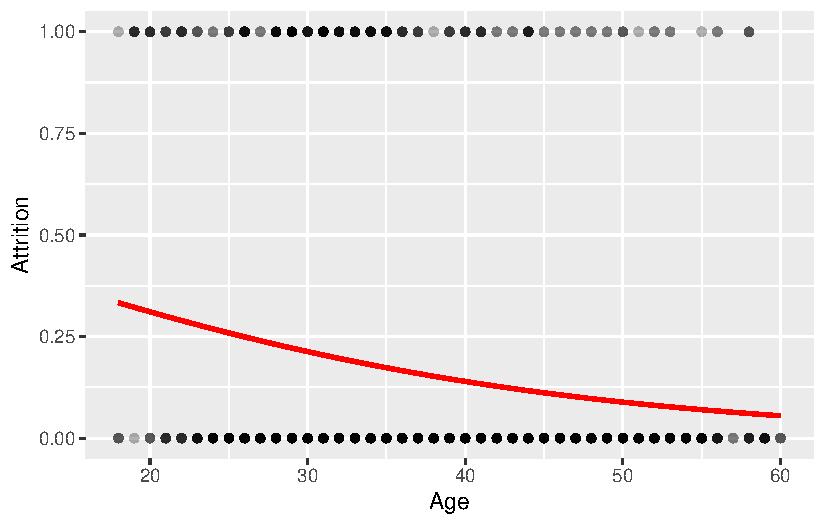
\includegraphics{./logistisk_regresjon_files/figure-pdf/unnamed-chunk-9-1.pdf}

}

\end{figure}

Du synes sikkert dette plottet ser litt rart ut. Bytt ut geom\_point()
med følgende: \texttt{geom\_jitter(height\ =\ .02,\ alpha=.3)} så skal
du få omtrent følgende resultat:

\begin{Shaded}
\begin{Highlighting}[]
\FunctionTok{ggplot}\NormalTok{(training, }\FunctionTok{aes}\NormalTok{(}\AttributeTok{x=}\NormalTok{Age, }\AttributeTok{y=}\NormalTok{Attrition))}\SpecialCharTok{+} 
  \FunctionTok{geom\_jitter}\NormalTok{(}\AttributeTok{height =}\NormalTok{ .}\DecValTok{02}\NormalTok{, }\AttributeTok{alpha=}\NormalTok{.}\DecValTok{3}\NormalTok{)}\SpecialCharTok{+} 
  \FunctionTok{stat\_smooth}\NormalTok{(}\AttributeTok{method=}\StringTok{"glm"}\NormalTok{, }\AttributeTok{method.args=}\FunctionTok{list}\NormalTok{(}\AttributeTok{family=}\StringTok{"binomial"}\NormalTok{), }\AttributeTok{se=}\ConstantTok{FALSE}\NormalTok{, }\AttributeTok{col=}\StringTok{"red"}\NormalTok{) }
\end{Highlighting}
\end{Shaded}

\begin{figure}[H]

{\centering 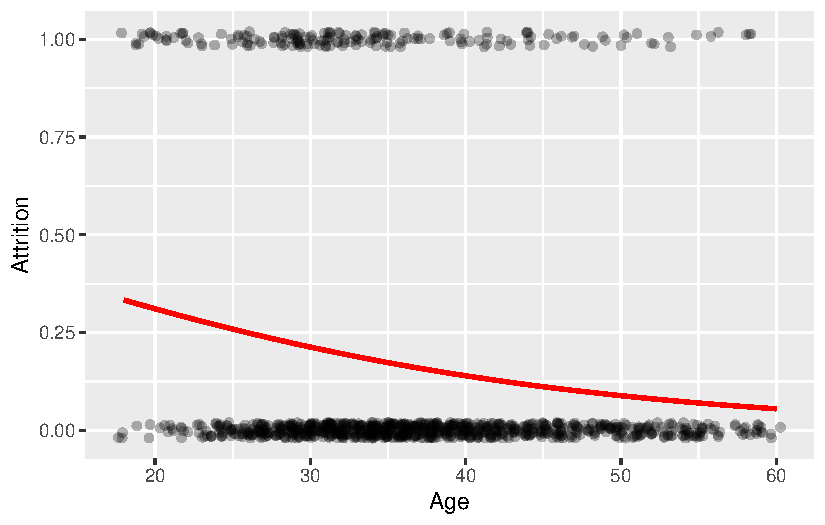
\includegraphics{./logistisk_regresjon_files/figure-pdf/unnamed-chunk-10-1.pdf}

}

\end{figure}

Det ser muligens fremdels rart ut, men litt tydeligere, kanskje.

Her er en variant der andelen som slutter i jobben er regnet ut for
hvert alderstrinn. Da er utfallsvariabelen en andel som er litt enklere
å tolke når det plottes, og regresjonslinjen er den samme.

\begin{Shaded}
\begin{Highlighting}[]
\NormalTok{training\_p }\OtherTok{\textless{}{-}}\NormalTok{ training }\SpecialCharTok{\%\textgreater{}\%} 
  \FunctionTok{group\_by}\NormalTok{(Age) }\SpecialCharTok{\%\textgreater{}\%} 
  \FunctionTok{summarise}\NormalTok{(}\AttributeTok{Attrition =} \FunctionTok{mean}\NormalTok{(Attrition }\SpecialCharTok{==} \DecValTok{1}\NormalTok{)) }
\FunctionTok{ggplot}\NormalTok{(training\_p, }\FunctionTok{aes}\NormalTok{(}\AttributeTok{x=}\NormalTok{Age, }\AttributeTok{y=}\NormalTok{Attrition))}\SpecialCharTok{+} 
  \FunctionTok{geom\_point}\NormalTok{()}\SpecialCharTok{+} 
  \FunctionTok{stat\_smooth}\NormalTok{(}\AttributeTok{method=}\StringTok{"glm"}\NormalTok{, }\AttributeTok{method.args=}\FunctionTok{list}\NormalTok{(}\AttributeTok{family=}\StringTok{"binomial"}\NormalTok{), }\AttributeTok{se=}\ConstantTok{FALSE}\NormalTok{, }\AttributeTok{col=}\StringTok{"red"}\NormalTok{) }
\end{Highlighting}
\end{Shaded}

\begin{figure}[H]

{\centering 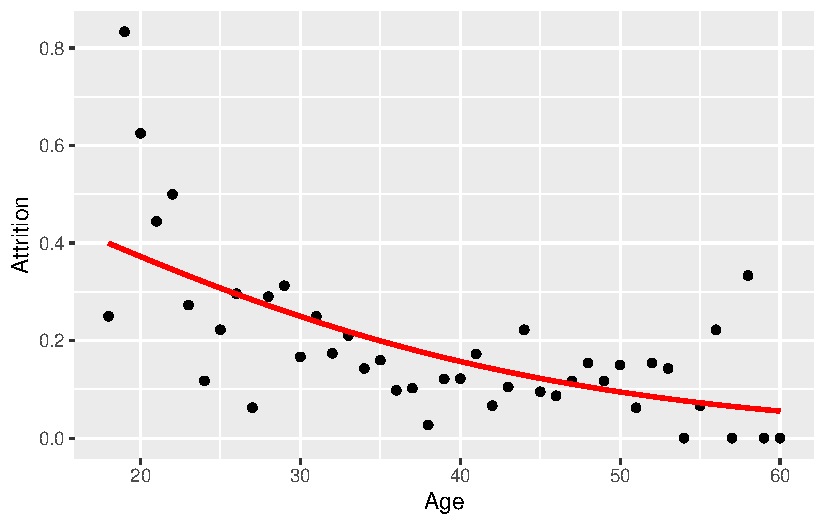
\includegraphics{./logistisk_regresjon_files/figure-pdf/unnamed-chunk-11-1.pdf}

}

\end{figure}

\hypertarget{enkel-logistisk-regresjon}{%
\subsection{Enkel logistisk regresjon}\label{enkel-logistisk-regresjon}}

\begin{Shaded}
\begin{Highlighting}[]
\NormalTok{est\_logit }\OtherTok{\textless{}{-}} \FunctionTok{glm}\NormalTok{(Attrition }\SpecialCharTok{\textasciitilde{}}\NormalTok{ Age, }\AttributeTok{data =}\NormalTok{ attrition, }\AttributeTok{family =} \StringTok{"binomial"}\NormalTok{)}
\FunctionTok{summary}\NormalTok{(est\_logit)}
\end{Highlighting}
\end{Shaded}

\begin{verbatim}

Call:
glm(formula = Attrition ~ Age, family = "binomial", data = attrition)

Deviance Residuals: 
    Min       1Q   Median       3Q      Max  
-0.8854  -0.6446  -0.5451  -0.4155   2.4008  

Coefficients:
            Estimate Std. Error z value Pr(>|z|)    
(Intercept)  0.20620    0.30599   0.674      0.5    
Age         -0.05225    0.00870  -6.006 1.91e-09 ***
---
Signif. codes:  0 '***' 0.001 '**' 0.01 '*' 0.05 '.' 0.1 ' ' 1

(Dispersion parameter for binomial family taken to be 1)

    Null deviance: 1298.6  on 1469  degrees of freedom
Residual deviance: 1259.1  on 1468  degrees of freedom
AIC: 1263.1

Number of Fisher Scoring iterations: 4
\end{verbatim}

\hypertarget{prediksjon}{%
\subsubsection{Prediksjon}\label{prediksjon}}

\begin{Shaded}
\begin{Highlighting}[]
\NormalTok{attrition\_pred }\OtherTok{\textless{}{-}}\NormalTok{ attrition }\SpecialCharTok{\%\textgreater{}\%} 
  \FunctionTok{mutate}\NormalTok{(}\AttributeTok{prob =} \FunctionTok{predict}\NormalTok{(est\_logit, }\AttributeTok{type =} \StringTok{"response"}\NormalTok{))}
\end{Highlighting}
\end{Shaded}

\hypertarget{roc-og-auc}{%
\subsubsection{ROC og AUC}\label{roc-og-auc}}

\begin{Shaded}
\begin{Highlighting}[]
\NormalTok{ROC }\OtherTok{\textless{}{-}} \FunctionTok{roc}\NormalTok{( attrition\_pred}\SpecialCharTok{$}\NormalTok{Attrition, attrition\_pred}\SpecialCharTok{$}\NormalTok{prob )}
\end{Highlighting}
\end{Shaded}

\begin{verbatim}
Setting levels: control = No, case = Yes
\end{verbatim}

\begin{verbatim}
Setting direction: controls < cases
\end{verbatim}

\begin{Shaded}
\begin{Highlighting}[]
\NormalTok{df }\OtherTok{\textless{}{-}} \FunctionTok{data.frame}\NormalTok{(}\AttributeTok{Sensitivity =}\NormalTok{ ROC}\SpecialCharTok{$}\NormalTok{sensitivities, }
                 \AttributeTok{Specificity =}\NormalTok{ ROC}\SpecialCharTok{$}\NormalTok{specificities)}

\FunctionTok{ggplot}\NormalTok{(df, }\FunctionTok{aes}\NormalTok{(}\AttributeTok{y =}\NormalTok{ Sensitivity, }\AttributeTok{x=}\NormalTok{ (}\DecValTok{1}\SpecialCharTok{{-}}\NormalTok{Specificity))) }\SpecialCharTok{+} 
  \FunctionTok{geom\_line}\NormalTok{() }\SpecialCharTok{+} 
  \FunctionTok{geom\_abline}\NormalTok{(}\AttributeTok{intercept =} \DecValTok{0}\NormalTok{, }\AttributeTok{slope =} \DecValTok{1}\NormalTok{, }\AttributeTok{col =} \StringTok{"gray"}\NormalTok{)}\SpecialCharTok{+}
  \FunctionTok{coord\_equal}\NormalTok{()}
\end{Highlighting}
\end{Shaded}

\begin{figure}[H]

{\centering 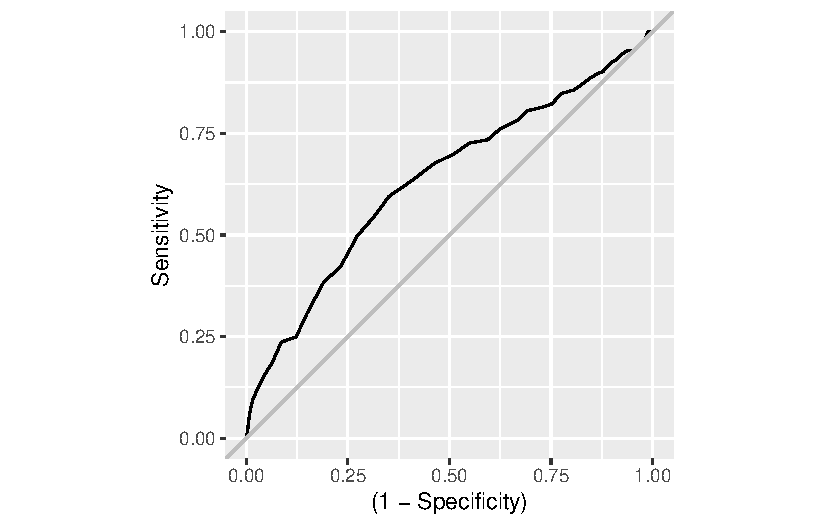
\includegraphics{./logistisk_regresjon_files/figure-pdf/unnamed-chunk-14-1.pdf}

}

\end{figure}

Area under the curve er 0.634.

\hypertarget{multippel-logistisk-regresjon}{%
\subsection{Multippel logistisk
regresjon}\label{multippel-logistisk-regresjon}}

\begin{Shaded}
\begin{Highlighting}[]
\NormalTok{est\_multlogit }\OtherTok{\textless{}{-}} \FunctionTok{glm}\NormalTok{(Attrition }\SpecialCharTok{\textasciitilde{}}\NormalTok{ ., }\AttributeTok{data =}\NormalTok{ attrition, }\AttributeTok{family =} \StringTok{"binomial"}\NormalTok{)}
\FunctionTok{summary}\NormalTok{(est\_multlogit)}
\end{Highlighting}
\end{Shaded}

\begin{verbatim}

Call:
glm(formula = Attrition ~ ., family = "binomial", data = attrition)

Deviance Residuals: 
    Min       1Q   Median       3Q      Max  
-1.6141  -0.4811  -0.2529  -0.0906   3.4189  

Coefficients:
                                   Estimate Std. Error z value Pr(>|z|)    
(Intercept)                      -1.140e+01  6.307e+02  -0.018 0.985578    
Age                              -3.152e-02  1.359e-02  -2.320 0.020363 *  
BusinessTravelTravel_Frequently   1.909e+00  4.119e-01   4.635 3.57e-06 ***
BusinessTravelTravel_Rarely       1.027e+00  3.798e-01   2.704 0.006859 ** 
DailyRate                        -2.843e-04  2.204e-04  -1.290 0.197098    
DepartmentResearch & Development  1.374e+01  6.307e+02   0.022 0.982626    
DepartmentSales                   1.360e+01  6.307e+02   0.022 0.982799    
DistanceFromHome                  4.585e-02  1.079e-02   4.250 2.14e-05 ***
Education                         1.148e-02  8.800e-02   0.130 0.896204    
EducationFieldLife Sciences      -7.514e-01  8.068e-01  -0.931 0.351681    
EducationFieldMarketing          -3.627e-01  8.555e-01  -0.424 0.671600    
EducationFieldMedical            -8.452e-01  8.063e-01  -1.048 0.294569    
EducationFieldOther              -7.906e-01  8.663e-01  -0.913 0.361458    
EducationFieldTechnical Degree    1.736e-01  8.247e-01   0.210 0.833318    
EmployeeNumber                   -1.540e-04  1.518e-04  -1.015 0.310159    
EnvironmentSatisfaction          -4.341e-01  8.301e-02  -5.229 1.70e-07 ***
GenderMale                        3.992e-01  1.847e-01   2.161 0.030676 *  
HourlyRate                        1.158e-03  4.413e-03   0.262 0.793070    
JobInvolvement                   -5.269e-01  1.227e-01  -4.294 1.76e-05 ***
JobLevel                         -9.377e-02  3.164e-01  -0.296 0.766941    
JobRoleHuman Resources            1.502e+01  6.307e+02   0.024 0.981001    
JobRoleLaboratory Technician      1.486e+00  4.858e-01   3.059 0.002224 ** 
JobRoleManager                    3.017e-01  8.904e-01   0.339 0.734739    
JobRoleManufacturing Director     2.462e-01  5.345e-01   0.461 0.645077    
JobRoleResearch Director         -1.133e+00  1.007e+00  -1.125 0.260580    
JobRoleResearch Scientist         5.373e-01  4.972e-01   1.081 0.279882    
JobRoleSales Executive            1.183e+00  1.126e+00   1.051 0.293191    
JobRoleSales Representative       2.135e+00  1.180e+00   1.808 0.070534 .  
JobSatisfaction                  -4.143e-01  8.152e-02  -5.082 3.74e-07 ***
MaritalStatusMarried              3.371e-01  2.670e-01   1.263 0.206724    
MaritalStatusSingle               1.174e+00  3.463e-01   3.389 0.000701 ***
MonthlyIncome                     1.347e-05  8.148e-05   0.165 0.868699    
MonthlyRate                       5.612e-06  1.253e-05   0.448 0.654285    
NumCompaniesWorked                1.945e-01  3.884e-02   5.008 5.50e-07 ***
OverTimeYes                       1.979e+00  1.939e-01  10.209  < 2e-16 ***
PercentSalaryHike                -2.331e-02  3.935e-02  -0.592 0.553532    
PerformanceRating                 1.165e-01  3.992e-01   0.292 0.770379    
RelationshipSatisfaction         -2.654e-01  8.292e-02  -3.201 0.001368 ** 
StockOptionLevel                 -1.930e-01  1.587e-01  -1.216 0.224040    
TotalWorkingYears                -5.992e-02  2.934e-02  -2.042 0.041120 *  
TrainingTimesLastYear            -1.884e-01  7.315e-02  -2.576 0.010002 *  
WorkLifeBalance                  -3.725e-01  1.242e-01  -2.999 0.002705 ** 
YearsAtCompany                    9.610e-02  3.891e-02   2.470 0.013509 *  
YearsInCurrentRole               -1.513e-01  4.553e-02  -3.323 0.000890 ***
YearsSinceLastPromotion           1.735e-01  4.242e-02   4.090 4.31e-05 ***
YearsWithCurrManager             -1.367e-01  4.703e-02  -2.907 0.003655 ** 
---
Signif. codes:  0 '***' 0.001 '**' 0.01 '*' 0.05 '.' 0.1 ' ' 1

(Dispersion parameter for binomial family taken to be 1)

    Null deviance: 1298.58  on 1469  degrees of freedom
Residual deviance:  857.98  on 1424  degrees of freedom
AIC: 949.98

Number of Fisher Scoring iterations: 15
\end{verbatim}

\hypertarget{prediksjon-1}{%
\subsubsection{Prediksjon}\label{prediksjon-1}}

\begin{Shaded}
\begin{Highlighting}[]
\NormalTok{attrition\_pred }\OtherTok{\textless{}{-}}\NormalTok{ attrition }\SpecialCharTok{\%\textgreater{}\%} 
  \FunctionTok{mutate}\NormalTok{(}\AttributeTok{prob =} \FunctionTok{predict}\NormalTok{(est\_multlogit, }\AttributeTok{type =} \StringTok{"response"}\NormalTok{)) }
\end{Highlighting}
\end{Shaded}

\hypertarget{roc-og-auc-1}{%
\subsubsection{ROC og AUC}\label{roc-og-auc-1}}

Funksjonen \texttt{roc()} gjør utregningene som trengs for ROC-kurven
basert på observert utfall og predikerte sannsynligheter.

OBS! Man må man angi data som \emph{første} argument i funksjonen
\texttt{roc()}, deretter observerte utfall og til sist predikert
sannsynlighet. Rekkefølgen er viktig!

Det går an å få ut plottet med en quick-and-dirty versjon med
\texttt{plot(ROC)}, men det blir penere med bruk av \texttt{ggplot()}
slik som er gjort nedenfor. Det krever at man lager en data.frame først
ved å plukke ut de relevante tallene fra ROC-objektet. (Men layout er
strengt tatt ikke viktig i dette kurset).

\begin{Shaded}
\begin{Highlighting}[]
\NormalTok{ROC }\OtherTok{\textless{}{-}} \FunctionTok{roc}\NormalTok{(attrition\_pred, Attrition, prob)}
\end{Highlighting}
\end{Shaded}

\begin{verbatim}
Setting levels: control = No, case = Yes
\end{verbatim}

\begin{verbatim}
Setting direction: controls < cases
\end{verbatim}

\begin{Shaded}
\begin{Highlighting}[]
\NormalTok{df }\OtherTok{\textless{}{-}} \FunctionTok{data.frame}\NormalTok{(}\AttributeTok{Sensitivity =}\NormalTok{ ROC}\SpecialCharTok{$}\NormalTok{sensitivities, }
                 \AttributeTok{Specificity =}\NormalTok{ ROC}\SpecialCharTok{$}\NormalTok{specificities)}

\FunctionTok{ggplot}\NormalTok{(df, }\FunctionTok{aes}\NormalTok{(}\AttributeTok{y =}\NormalTok{ Sensitivity, }\AttributeTok{x=}\NormalTok{ (}\DecValTok{1}\SpecialCharTok{{-}}\NormalTok{Specificity))) }\SpecialCharTok{+} 
  \FunctionTok{geom\_line}\NormalTok{() }\SpecialCharTok{+} 
  \FunctionTok{geom\_abline}\NormalTok{(}\AttributeTok{intercept =} \DecValTok{0}\NormalTok{, }\AttributeTok{slope =} \DecValTok{1}\NormalTok{, }\AttributeTok{col =} \StringTok{"gray"}\NormalTok{)}\SpecialCharTok{+}
  \FunctionTok{coord\_equal}\NormalTok{()}
\end{Highlighting}
\end{Shaded}

\begin{figure}[H]

{\centering 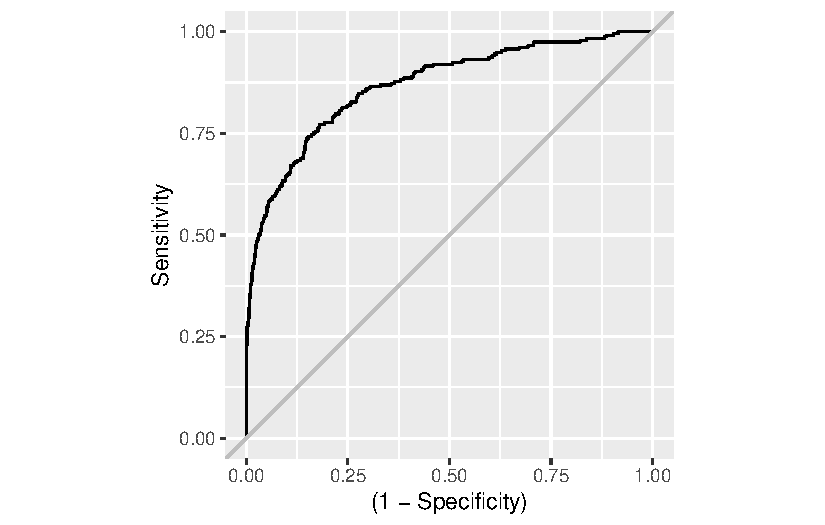
\includegraphics{./logistisk_regresjon_files/figure-pdf/unnamed-chunk-17-1.pdf}

}

\end{figure}

Vi kan da få rapportert arealet under kurven med \texttt{auc()} slik:

\begin{Shaded}
\begin{Highlighting}[]
\FunctionTok{auc}\NormalTok{(ROC)}
\end{Highlighting}
\end{Shaded}

\begin{verbatim}
Area under the curve: 0.8687
\end{verbatim}

Når arealet under kurven (AUC) er 0.869 er det vesentlig bedre
prediksjon enn den enkle modellen.

\hypertarget{oppgaver-tmpuxe5}{%
\section{Oppgaver tmpå}\label{oppgaver-tmpuxe5}}

\begin{itemize}
\tightlist
\item
  Du gjorde et valg av cut-off ovenfor. En måte for å vurdere
  klassifiseringen er å sammenligne det resultatet med de observerte
  dataene. Lag en tabell for din klassifisering vs observert slik:\\
  table(klass, training\$Attrition) Synes du dette ble presist nok? Prøv
  gjerne å endre cut-off for klassifiseringen.
\end{itemize}

Slike tabeller skal vi snakke mer om de kommende gangen. Det kalles
gjerne en «confusion matrix».

\leavevmode\vadjust pre{\hypertarget{exr-stepw1}{}}%
\begin{exercise}[]\label{exr-stepw1}

Det finnes prosedyrer for automatisk seleksjon av variable. Da søkes det
gjennom de spennet av mulige modeller som oppgis og finner den modellen
som predikerer best. Oppgi den enkleste modellen du vil starte fra og
den mest kompliserte modellen du vil vurdere og estimer disse to
modellene.

\end{exercise}

En modell med kun konstantledd skrives med \texttt{\textasciitilde{}} 1
i formelen slik:
\texttt{null\_model\ \textless{}-\ glm(Attrition\ \textasciitilde{}\ 1,\ data\ =\ training,\ family\ =\ "binomial")}

Lag en mer komplisert formel. Ta med så mange prediktorer du vil! Gjerne
samspillsledd og polynomer også. Samspill:
\texttt{variabel1\ *\ variabel2}. Polynom, f.eks. kvadratledd:
\texttt{I(variabel\textbackslash{}\^{}2)}.

fmla\_full \textless- Attrition \textasciitilde{} \_\_\_\_\_\_\_\_\_
full\_model \textless- glm(\_\_\_\_\_ , data = \_\_\_\_\_\_,
family=``binomial'')

Med funksjonen step() søker R gjennom alle modellene. Bruk følgende kode
og endelig modell\\
step\_model \textless- step(null\_model,\\
scope = list(lower = null\_model,\\
upper = full\_model),\\
direction = ``forward'') Ta en titt på endelig resultat:\\
summary( \_\_\_\_\_\_ )

Bruk nå predict() som i oppgave en for predikere sannsynligheter, lag en
ROC curve og regn ut AUC.

\leavevmode\vadjust pre{\hypertarget{exr-stepw-test}{}}%
\begin{exercise}[]\label{exr-stepw-test}

Sjekk så mot test-data! Du har optimalisert en modell til å passe de
dataene du hadde. Hvordan vil det funke på nye data? Til dette bruker vi
det mindre datasettet testing som du lagde over.

\begin{itemize}
\tightlist
\item
  Bruk step\_model som du lagde i forrige oppgave og prediker for nye
  data. Bruk predict(), men husk å spesifisere newdata=testing.\\
\item
  Lag så en ROC curve og regn ut AUC på nytt!
\end{itemize}

\end{exercise}

\hypertarget{oppgaver-2}{%
\section{Oppgaver}\label{oppgaver-2}}

Disse oppgavene vil være ganske tilsvarende som for oppgavene med lineær
regresjon. Men du skal nå bruke logistisk regresjon med tilhørende
teknikker og vurderinger.

\leavevmode\vadjust pre{\hypertarget{exr-ols-eksplisitt}{}}%
\begin{exercise}[]\label{exr-ols-eksplisitt}

Velg et datasettet og formuler hva en prediksjonsmodell for disse
dataene kan kunne brukes til. Du må velge et datasett som har en
utfallsvariabel som er kategorisk eller evt. omkode utfallsvariabelen
til kategorier. Se for deg at tiltak du foreslår vil altså ha faktiske
konsekvenser, så gjør en vurdering av hvorvidt feilprediksjoner vil være
problematiske og i så fall på hvilken måte. Vurder mulighetene for feil
opp mot gevinst ved riktig prediksjon.

Merk: som i tidligere oppgaver er det ikke viktig at anvendelsen skal
være realistisk, men du må alltid ta konsekvensen i vurderingene.

\end{exercise}

\leavevmode\vadjust pre{\hypertarget{exr-logit-split}{}}%
\begin{exercise}[]\label{exr-logit-split}

Last inn valgte datasett og splitt i et training og et testing datasett.
Sett splitten ved .70. Bruk training-data til å gjøre deg kjent med
dataene og estimere modellene. Ikke bruk testing-dataene inntil du får
beskjed om det.

\end{exercise}

\leavevmode\vadjust pre{\hypertarget{exr-logit-sepaa}{}}%
\begin{exercise}[]\label{exr-logit-sepaa}

Gjør deg kjent med innholdet i disse training-dataene. Du kan gjøre
f.eks. følgende:

\begin{enumerate}
\def\labelenumi{\alph{enumi})}
\tightlist
\item
  Bruk \texttt{glimpse()} og \texttt{skim()} til å få oversikt over
  innholdet i datasettet
\item
  Hvis det er noen variable du ikke kommer til å bruke, slett gjerne
  disse med en gang
\item
  Lag noen tabeller og plot som viser hvordan utfallsvariabelen er
  fordelt etter andre variable
\end{enumerate}

\end{exercise}

\leavevmode\vadjust pre{\hypertarget{exr-logit-train}{}}%
\begin{exercise}[]\label{exr-logit-train}

Estimer flere lineær regresjonsmodeller med et fåtall prediktorer. Gjør
et utvalg av de variablene du mener er mest relevant for å forklare
utfallet. Estimer flere lineære regresjonsmodeller for å predikere
utfallet, og sammenlign hvor gode prediksjoner disse gir. Mest relevante
statistikker er \(r^2\) og AUC. Regn også ut RMSE.

\begin{enumerate}
\def\labelenumi{\alph{enumi})}
\tightlist
\item
  Velg ut tre forklaringsvariable og estimer en regresjonsmodell
\item
  Estimer en ny modell med alle variable i datasettet
\item
  Estimer en ny modell og inkluder noen få polynomer og/eller
  interaksjonsledd
\item
  Gjør et automatisk modellsøk
\end{enumerate}

Lag gjerne noen plot av ROC-curve for i hvert fall noen av modellene
slik at du får en følelse med hva AUC egentlig betyr. Plot også
predikert verdi mot observert verdi og gjør en vurdering av RMSE.

\end{exercise}

\leavevmode\vadjust pre{\hypertarget{exr-logit-test}{}}%
\begin{exercise}[]\label{exr-logit-test}

I forrige oppgave brukte du testing-datasettet til både å estimere
modellene og vurdere resultatet. Nå skal du bruke testing-datasettet til
å vurdere de samme resultatene. Dette gjør du ved å predikere på
testing-datasettet og regne ut AUC og RMSE for disse dataene. For hver
modell i forrige oppgave, gjør som følger:

\begin{enumerate}
\def\labelenumi{\alph{enumi})}
\tightlist
\item
  Prediker utfallet på testing-datasettet
\item
  Regn ut AUC
\item
  Hvor stor er \emph{endringen} i AUC er fra resultatene når du brukte
  training-datasettet?
\end{enumerate}

Vurdering: En mer komplisert modell beskriver dataene bedre. Men er det
like stor \emph{endring} i AUC og RMSE for enkle og mer kompliserte
modeller? Beskriv hva du ser og gi en forklaring.

\end{exercise}

\bookmarksetup{startatroot}

\hypertarget{klassifikasjonstruxe6r}{%
\chapter{Klassifikasjonstrær}\label{klassifikasjonstruxe6r}}

\begin{Shaded}
\begin{Highlighting}[]
\FunctionTok{library}\NormalTok{(tidyverse) }
\FunctionTok{library}\NormalTok{(rpart)      }\CommentTok{\# funksjoner for CART }
\FunctionTok{library}\NormalTok{(rpart.plot) }\CommentTok{\# funksjon for å plotte CART }
\FunctionTok{library}\NormalTok{(caret)      }\CommentTok{\# inneholder funksjon for confusion matrix }
\FunctionTok{library}\NormalTok{(skimr)      }\CommentTok{\# funksjonen skim()}
\end{Highlighting}
\end{Shaded}

Vi skal her bruke datasettet \textbf{credit} fra Canvas. Dataene er en
banks kundehistorikk for kreditt for 1000 kunder. Variabelen
\emph{default}\footnote{Begrepet ``default'' på engelsk kan bety å ikke
  holde en forpliktelse, men i software kan det bety forhåndsvalg. Dette
  kan være forvirrende akkurat her. Du kan godt endre variabelnavnet
  hvis du vil.} er «yes» hvis tilbakebetaling som avtalt og «no» hvis
ikke. Dette er utfallsvariabelen. Øvrige variable er rimelig
selvforklarende etter variabelnavn. Målet er å lage et system for hvilke
nye kunder som skal få innvilget kreditt.

\begin{Shaded}
\begin{Highlighting}[]
\NormalTok{credit }\OtherTok{\textless{}{-}} \FunctionTok{read.csv}\NormalTok{(}\StringTok{"../data/credit.csv"}\NormalTok{, }\AttributeTok{stringsAsFactors =} \ConstantTok{TRUE}\NormalTok{) }

\FunctionTok{skim}\NormalTok{(credit)}
\end{Highlighting}
\end{Shaded}

\begin{longtable}[]{@{}ll@{}}
\caption{Data summary}\tabularnewline
\toprule()
\endhead
Name & credit \\
Number of rows & 1000 \\
Number of columns & 17 \\
\_\_\_\_\_\_\_\_\_\_\_\_\_\_\_\_\_\_\_\_\_\_\_ & \\
Column type frequency: & \\
factor & 10 \\
numeric & 7 \\
\_\_\_\_\_\_\_\_\_\_\_\_\_\_\_\_\_\_\_\_\_\_\_\_ & \\
Group variables & None \\
\bottomrule()
\end{longtable}

\textbf{Variable type: factor}

\begin{longtable}[]{@{}
  >{\raggedright\arraybackslash}p{(\columnwidth - 10\tabcolsep) * \real{0.2000}}
  >{\raggedleft\arraybackslash}p{(\columnwidth - 10\tabcolsep) * \real{0.1000}}
  >{\raggedleft\arraybackslash}p{(\columnwidth - 10\tabcolsep) * \real{0.1400}}
  >{\raggedright\arraybackslash}p{(\columnwidth - 10\tabcolsep) * \real{0.0800}}
  >{\raggedleft\arraybackslash}p{(\columnwidth - 10\tabcolsep) * \real{0.0900}}
  >{\raggedright\arraybackslash}p{(\columnwidth - 10\tabcolsep) * \real{0.3900}}@{}}
\toprule()
\begin{minipage}[b]{\linewidth}\raggedright
skim\_variable
\end{minipage} & \begin{minipage}[b]{\linewidth}\raggedleft
n\_missing
\end{minipage} & \begin{minipage}[b]{\linewidth}\raggedleft
complete\_rate
\end{minipage} & \begin{minipage}[b]{\linewidth}\raggedright
ordered
\end{minipage} & \begin{minipage}[b]{\linewidth}\raggedleft
n\_unique
\end{minipage} & \begin{minipage}[b]{\linewidth}\raggedright
top\_counts
\end{minipage} \\
\midrule()
\endhead
checking\_balance & 0 & 1 & FALSE & 4 & unk: 394, \textless{} 0: 274, 1
-: 269, \textgreater{} 2: 63 \\
credit\_history & 0 & 1 & FALSE & 5 & goo: 530, cri: 293, poo: 88, ver:
49 \\
purpose & 0 & 1 & FALSE & 6 & fur: 473, car: 337, bus: 97, edu: 59 \\
savings\_balance & 0 & 1 & FALSE & 5 & \textless{} 1: 603, unk: 183,
100: 103, 500: 63 \\
employment\_duration & 0 & 1 & FALSE & 5 & 1 -: 339, \textgreater{} 7:
253, 4 -: 174, \textless{} 1: 172 \\
other\_credit & 0 & 1 & FALSE & 3 & non: 814, ban: 139, sto: 47 \\
housing & 0 & 1 & FALSE & 3 & own: 713, ren: 179, oth: 108 \\
job & 0 & 1 & FALSE & 4 & ski: 630, uns: 200, man: 148, une: 22 \\
phone & 0 & 1 & FALSE & 2 & no: 596, yes: 404 \\
default & 0 & 1 & FALSE & 2 & no: 700, yes: 300 \\
\bottomrule()
\end{longtable}

\textbf{Variable type: numeric}

\begin{longtable}[]{@{}
  >{\raggedright\arraybackslash}p{(\columnwidth - 20\tabcolsep) * \real{0.2121}}
  >{\raggedleft\arraybackslash}p{(\columnwidth - 20\tabcolsep) * \real{0.1010}}
  >{\raggedleft\arraybackslash}p{(\columnwidth - 20\tabcolsep) * \real{0.1414}}
  >{\raggedleft\arraybackslash}p{(\columnwidth - 20\tabcolsep) * \real{0.0808}}
  >{\raggedleft\arraybackslash}p{(\columnwidth - 20\tabcolsep) * \real{0.0808}}
  >{\raggedleft\arraybackslash}p{(\columnwidth - 20\tabcolsep) * \real{0.0404}}
  >{\raggedleft\arraybackslash}p{(\columnwidth - 20\tabcolsep) * \real{0.0707}}
  >{\raggedleft\arraybackslash}p{(\columnwidth - 20\tabcolsep) * \real{0.0707}}
  >{\raggedleft\arraybackslash}p{(\columnwidth - 20\tabcolsep) * \real{0.0808}}
  >{\raggedleft\arraybackslash}p{(\columnwidth - 20\tabcolsep) * \real{0.0606}}
  >{\raggedright\arraybackslash}p{(\columnwidth - 20\tabcolsep) * \real{0.0606}}@{}}
\toprule()
\begin{minipage}[b]{\linewidth}\raggedright
skim\_variable
\end{minipage} & \begin{minipage}[b]{\linewidth}\raggedleft
n\_missing
\end{minipage} & \begin{minipage}[b]{\linewidth}\raggedleft
complete\_rate
\end{minipage} & \begin{minipage}[b]{\linewidth}\raggedleft
mean
\end{minipage} & \begin{minipage}[b]{\linewidth}\raggedleft
sd
\end{minipage} & \begin{minipage}[b]{\linewidth}\raggedleft
p0
\end{minipage} & \begin{minipage}[b]{\linewidth}\raggedleft
p25
\end{minipage} & \begin{minipage}[b]{\linewidth}\raggedleft
p50
\end{minipage} & \begin{minipage}[b]{\linewidth}\raggedleft
p75
\end{minipage} & \begin{minipage}[b]{\linewidth}\raggedleft
p100
\end{minipage} & \begin{minipage}[b]{\linewidth}\raggedright
hist
\end{minipage} \\
\midrule()
\endhead
months\_loan\_duration & 0 & 1 & 20.90 & 12.06 & 4 & 12.0 & 18.0 & 24.00
& 72 & ▇▇▂▁▁ \\
amount & 0 & 1 & 3271.26 & 2822.74 & 250 & 1365.5 & 2319.5 & 3972.25 &
18424 & ▇▂▁▁▁ \\
percent\_of\_income & 0 & 1 & 2.97 & 1.12 & 1 & 2.0 & 3.0 & 4.00 & 4 &
▂▃▁▂▇ \\
years\_at\_residence & 0 & 1 & 2.85 & 1.10 & 1 & 2.0 & 3.0 & 4.00 & 4 &
▂▆▁▃▇ \\
age & 0 & 1 & 35.55 & 11.38 & 19 & 27.0 & 33.0 & 42.00 & 75 & ▇▆▃▁▁ \\
existing\_loans\_count & 0 & 1 & 1.41 & 0.58 & 1 & 1.0 & 1.0 & 2.00 & 4
& ▇▅▁▁▁ \\
dependents & 0 & 1 & 1.16 & 0.36 & 1 & 1.0 & 1.0 & 1.00 & 2 & ▇▁▁▁▂ \\
\bottomrule()
\end{longtable}

Vi splitter først datasettet i to deler: en til training og en til
testing.

\begin{Shaded}
\begin{Highlighting}[]
\NormalTok{grense }\OtherTok{\textless{}{-}} \FloatTok{0.7}
\NormalTok{lottery }\OtherTok{\textless{}{-}} \FunctionTok{runif}\NormalTok{(}\AttributeTok{n =} \FunctionTok{nrow}\NormalTok{(credit))}

\NormalTok{training }\OtherTok{\textless{}{-}} \FunctionTok{filter}\NormalTok{(credit, lottery }\SpecialCharTok{\textless{}}\NormalTok{ grense)}
\NormalTok{testing  }\OtherTok{\textless{}{-}} \FunctionTok{filter}\NormalTok{(credit, lottery }\SpecialCharTok{\textgreater{}=}\NormalTok{ grense)}
\end{Highlighting}
\end{Shaded}

Vi starter med å inkludere noen få variable som gir en oversiktlig
illustrasjon. Utfallsvariabel og prediktorer spesifiseres som en formel
på samme måte som for regresjon. Siden vi her har en klassifikasjon må
vi spesifisere \texttt{method\ =\ "class"}. Hvis ikke vil
\texttt{rpart()} gjette hva slags modell (som kanskje er riktig), så du
kan få andre resultater enn du forventet.

\begin{Shaded}
\begin{Highlighting}[]
\NormalTok{credit\_tree }\OtherTok{\textless{}{-}} \FunctionTok{rpart}\NormalTok{(default }\SpecialCharTok{\textasciitilde{}}\NormalTok{ age }\SpecialCharTok{+}\NormalTok{ amount }\SpecialCharTok{+}\NormalTok{ percent\_of\_income }\SpecialCharTok{+}\NormalTok{ purpose }\SpecialCharTok{+}\NormalTok{ employment\_duration }\SpecialCharTok{+}\NormalTok{ housing, }
                     \AttributeTok{data=}\NormalTok{training, }\AttributeTok{method=}\StringTok{"class"}\NormalTok{)}
\FunctionTok{rpart.plot}\NormalTok{(credit\_tree)}
\end{Highlighting}
\end{Shaded}

\begin{figure}[H]

{\centering \includegraphics{./cart_files/figure-pdf/unnamed-chunk-4-1.pdf}

}

\end{figure}

Vi kan også få printet ut disse som tall i en tabell.

\begin{Shaded}
\begin{Highlighting}[]
\FunctionTok{rpart.rules}\NormalTok{(credit\_tree, }\AttributeTok{extra=}\DecValTok{4}\NormalTok{)  }
\end{Highlighting}
\end{Shaded}

\begin{verbatim}
 default    no yes                                                                                                                                                                                                                               
      no [1.00 .00] when age <  26       & amount is 3465 to 4042                                                                                                                                                                                
      no  [.83 .17] when age >=       26 & amount <  3781         & employment_duration is > 7 years or 1 - 4 years or 4 - 7 years                                                                                                               
      no  [.75 .25] when age >=       26 & amount >=         3781 & employment_duration is > 7 years or 1 - 4 years or 4 - 7 years                                                              & housing is       other & percent_of_income <  3
      no  [.73 .27] when age <  26       & amount <  1804                                                                          & purpose is business or furniture/appliances or renovations                                                  
      no  [.71 .29] when age >=       26 & amount >=         3781 & employment_duration is > 7 years or 1 - 4 years or 4 - 7 years                                                              & housing is own or rent                         
      no  [.63 .37] when age >=       26                          & employment_duration is                  < 1 year or unemployed & purpose is             car or car0 or furniture/appliances                                                  
      no  [.61 .39] when age is 23 to 26 & amount is 1804 to 3465                                                                  & purpose is business or furniture/appliances or renovations                                                  
     yes  [.36 .64] when age <  26       & amount <  3465                                                                          & purpose is                                car or education                                                  
     yes  [.31 .69] when age <  26       & amount >=         4042                                                                                                                                                                                
     yes  [.29 .71] when age >=       26                          & employment_duration is                  < 1 year or unemployed & purpose is            business or education or renovations                                                  
     yes  [.28 .72] when age >=       26 & amount >=         3781 & employment_duration is > 7 years or 1 - 4 years or 4 - 7 years                                                              & housing is       other & percent_of_income >= 3
     yes  [.18 .82] when age <  23       & amount is 1804 to 3465                                                                  & purpose is business or furniture/appliances or renovations                                                  
\end{verbatim}

Vi kan så skrive ut confusion matrix.

\begin{Shaded}
\begin{Highlighting}[]
\NormalTok{rpart\_class }\OtherTok{\textless{}{-}} \FunctionTok{predict}\NormalTok{(credit\_tree, }\AttributeTok{type=}\StringTok{"class"}\NormalTok{)}
\FunctionTok{table}\NormalTok{(rpart\_class, training}\SpecialCharTok{$}\NormalTok{default)}
\end{Highlighting}
\end{Shaded}

\begin{verbatim}
           
rpart_class  no yes
        no  458 139
        yes  29  68
\end{verbatim}

\begin{Shaded}
\begin{Highlighting}[]
\FunctionTok{confusionMatrix}\NormalTok{(rpart\_class, training}\SpecialCharTok{$}\NormalTok{default)}
\end{Highlighting}
\end{Shaded}

\begin{verbatim}
Confusion Matrix and Statistics

          Reference
Prediction  no yes
       no  458 139
       yes  29  68
                                          
               Accuracy : 0.7579          
                 95% CI : (0.7243, 0.7894)
    No Information Rate : 0.7017          
    P-Value [Acc > NIR] : 0.0005722       
                                          
                  Kappa : 0.3174          
                                          
 Mcnemar's Test P-Value : < 2.2e-16       
                                          
            Sensitivity : 0.9405          
            Specificity : 0.3285          
         Pos Pred Value : 0.7672          
         Neg Pred Value : 0.7010          
             Prevalence : 0.7017          
         Detection Rate : 0.6599          
   Detection Prevalence : 0.8602          
      Balanced Accuracy : 0.6345          
                                          
       'Positive' Class : no              
                                          
\end{verbatim}

\begin{Shaded}
\begin{Highlighting}[]
\NormalTok{rpart\_test }\OtherTok{\textless{}{-}} \FunctionTok{predict}\NormalTok{(credit\_tree, }\AttributeTok{newdata=}\NormalTok{testing, }\AttributeTok{type=}\StringTok{"class"}\NormalTok{)}
\FunctionTok{confusionMatrix}\NormalTok{(rpart\_test, testing}\SpecialCharTok{$}\NormalTok{default)}
\end{Highlighting}
\end{Shaded}

\begin{verbatim}
Confusion Matrix and Statistics

          Reference
Prediction  no yes
       no  188  78
       yes  25  15
                                          
               Accuracy : 0.6634          
                 95% CI : (0.6074, 0.7162)
    No Information Rate : 0.6961          
    P-Value [Acc > NIR] : 0.9032          
                                          
                  Kappa : 0.0523          
                                          
 Mcnemar's Test P-Value : 2.996e-07       
                                          
            Sensitivity : 0.8826          
            Specificity : 0.1613          
         Pos Pred Value : 0.7068          
         Neg Pred Value : 0.3750          
             Prevalence : 0.6961          
         Detection Rate : 0.6144          
   Detection Prevalence : 0.8693          
      Balanced Accuracy : 0.5220          
                                          
       'Positive' Class : no              
                                          
\end{verbatim}

\hypertarget{oppgaver-3}{%
\section{Oppgaver}\label{oppgaver-3}}

\leavevmode\vadjust pre{\hypertarget{exr-}{}}%
\begin{exercise}[]\label{exr-}

Gjenta oppgave 1, men basert på dine vurderinger i e) se om du klarer å
tune modellen mer i retning av ønsket cost-ratio. Bruk argumentene
prior, cp, minbucket og maxdepth.

\end{exercise}

\leavevmode\vadjust pre{\hypertarget{exr-}{}}%
\begin{exercise}[]\label{exr-}

Bruk datasettet credit til å predikere kredittverdighet for nye kunder.

\begin{enumerate}
\def\labelenumi{\alph{enumi})}
\tightlist
\item
  Spesifiser en formel med et fåtall variable og lag et
  klassifikasjonstre.
\item
  Plot med rpart.plot()
\item
  Bruk predict() til å klassifisere.
\item
  Lag en confusion matrix med table()
\item
  Gi en vurdering av resultatet.

  \begin{enumerate}
  \def\labelenumii{\arabic{enumii})}
  \tightlist
  \item
    Si noe om forholdet mellom resultat for training og testing
    datasett.
  \item
    Er cost-ratio ok fra bankens perspektiv?
  \item
    Er cost-ratio ok fra kundens perspektiv?
  \item
    Andre hensyn som bør spille inn her?
  \end{enumerate}
\end{enumerate}

\end{exercise}

\leavevmode\vadjust pre{\hypertarget{exr-}{}}%
\begin{exercise}[]\label{exr-}

Datafilen credit\_kunder.csv inneholder data om to lånesøkere: Ola
Normann og Kari Hansen.\\
Skal banken gi dem lån? Bruk foretrukne modell fra forrige oppgave.

\end{exercise}

\leavevmode\vadjust pre{\hypertarget{exr-}{}}%
\begin{exercise}[]\label{exr-}

Banker bruker slike systemer i dag i større eller mindre grad til
automatisere behandling av lånesøknader. (Men de bruker både rikere data
og mer avanserte algoritmer). I hvilken grad synes du slike systemer
kan/bør helautomatiseres? Bør det være reguleringer på hva slags data
som benyttes til slike systemer? Bør kunden få innsyn i algoritmen ved
avslag? Gi noen vurderinger av mulige fordeler og ulemper med tanke på
hvordan det kan slå ut for enkeltindivider.

\end{exercise}

\bookmarksetup{startatroot}

\hypertarget{bagging}{%
\chapter{Bagging}\label{bagging}}

\bookmarksetup{startatroot}

\hypertarget{introduksjon-til-bagging}{%
\chapter{Introduksjon til bagging}\label{introduksjon-til-bagging}}

\begin{Shaded}
\begin{Highlighting}[]
\CommentTok{\# Kilde: https://www.statology.org/bagging{-}in{-}r/ }

\FunctionTok{library}\NormalTok{(e1071)       }\CommentTok{\#for calculating variable importance}
\FunctionTok{library}\NormalTok{(caret)       }\CommentTok{\#for general model fitting}
\FunctionTok{library}\NormalTok{(rpart)       }\CommentTok{\#for fitting decision trees}
\FunctionTok{library}\NormalTok{(ipred)       }\CommentTok{\#for fitting bagged decision trees}

\NormalTok{credit }\OtherTok{\textless{}{-}} \FunctionTok{read.csv}\NormalTok{(}\StringTok{"../data/credit.csv"}\NormalTok{, }\AttributeTok{stringsAsFactors =} \ConstantTok{TRUE}\NormalTok{) }
\end{Highlighting}
\end{Shaded}

\hypertarget{oppgaver-4}{%
\section{Oppgaver}\label{oppgaver-4}}

\leavevmode\vadjust pre{\hypertarget{exr-}{}}%
\begin{exercise}[]\label{exr-}

Bruk bagging til å forbedre prediksjonene. Bruk samme formel, men bygg
150 trær.

\end{exercise}

\begin{solution}

\begin{Shaded}
\begin{Highlighting}[]
\NormalTok{fmla }\OtherTok{\textless{}{-}}\NormalTok{ default }\SpecialCharTok{\textasciitilde{}}\NormalTok{ age }\SpecialCharTok{+}\NormalTok{ amount }\SpecialCharTok{+}\NormalTok{ percent\_of\_income }\SpecialCharTok{+}\NormalTok{ purpose }\SpecialCharTok{+}\NormalTok{ employment\_duration }\SpecialCharTok{+}\NormalTok{ housing }

\NormalTok{fmla}
\end{Highlighting}
\end{Shaded}

\begin{verbatim}
default ~ age + amount + percent_of_income + purpose + employment_duration + 
    housing
\end{verbatim}

\begin{Shaded}
\begin{Highlighting}[]
\FunctionTok{set.seed}\NormalTok{(}\DecValTok{1}\NormalTok{)}
\NormalTok{bag }\OtherTok{\textless{}{-}} \FunctionTok{bagging}\NormalTok{(}
  \AttributeTok{formula =}\NormalTok{ fmla,}
  \AttributeTok{data =}\NormalTok{ credit,}
  \AttributeTok{nbagg =} \DecValTok{150}\NormalTok{,   }
  \AttributeTok{coob =} \ConstantTok{TRUE}\NormalTok{,}
  \AttributeTok{control =} \FunctionTok{rpart.control}\NormalTok{(}\AttributeTok{minsplit =} \DecValTok{2}\NormalTok{, }\AttributeTok{cp =} \DecValTok{0}\NormalTok{)}
\NormalTok{)}
\NormalTok{bag}
\end{Highlighting}
\end{Shaded}

\begin{verbatim}

Bagging classification trees with 150 bootstrap replications 

Call: bagging.data.frame(formula = fmla, data = credit, nbagg = 150, 
    coob = TRUE, control = rpart.control(minsplit = 2, cp = 0))

Out-of-bag estimate of misclassification error:  0.342 
\end{verbatim}

\end{solution}

\bookmarksetup{startatroot}

\hypertarget{random-forest}{%
\chapter{Random forest}\label{random-forest}}

Random forest bruker klassifikasjonstrær og bagging som byggestener. I
prinsippet er det ``bagged trees'', men i stedet for å bagge samme type
trær, så gjøres det en endring i hvert tre.

\begin{Shaded}
\begin{Highlighting}[]
\FunctionTok{library}\NormalTok{(tidyverse)}
\FunctionTok{library}\NormalTok{(rsample)}
\FunctionTok{library}\NormalTok{(fairmodels)}
\FunctionTok{library}\NormalTok{(randomForest)}
\FunctionTok{library}\NormalTok{(caret)}
\end{Highlighting}
\end{Shaded}

\hypertarget{eksempel}{%
\section{Eksempel}\label{eksempel}}

Leser inn Compas-dataene.

\begin{Shaded}
\begin{Highlighting}[]
\NormalTok{compas }\OtherTok{\textless{}{-}} \FunctionTok{readRDS}\NormalTok{(}\StringTok{"../data/compas.rds"}\NormalTok{)}
\FunctionTok{glimpse}\NormalTok{(compas)}
\end{Highlighting}
\end{Shaded}

\begin{verbatim}
Rows: 6,172
Columns: 7
$ Two_yr_Recidivism    <fct> 0, 1, 1, 0, 1, 0, 0, 0, 1, 0, 0, 1, 1, 0, 0, 1, 1~
$ Number_of_Priors     <int> 0, 0, 4, 0, 14, 3, 0, 0, 3, 0, 0, 1, 7, 0, 3, 6, ~
$ Age_Above_FourtyFive <fct> 1, 0, 0, 0, 0, 0, 0, 0, 0, 0, 0, 1, 0, 0, 0, 0, 0~
$ Age_Below_TwentyFive <fct> 0, 0, 1, 0, 0, 0, 0, 0, 1, 0, 0, 0, 0, 0, 0, 0, 0~
$ Misdemeanor          <fct> 0, 0, 0, 1, 0, 0, 1, 0, 1, 1, 0, 0, 0, 1, 0, 0, 0~
$ Ethnicity            <fct> Other, African_American, African_American, Other,~
$ Sex                  <fct> Male, Male, Male, Male, Male, Male, Female, Male,~
\end{verbatim}

Estimerer random forest med alle variable

\begin{Shaded}
\begin{Highlighting}[]
\FunctionTok{set.seed}\NormalTok{(}\DecValTok{4356}\NormalTok{)}
\NormalTok{rf }\OtherTok{\textless{}{-}} \FunctionTok{randomForest}\NormalTok{(Two\_yr\_Recidivism }\SpecialCharTok{\textasciitilde{}}\NormalTok{ . , }
                    \AttributeTok{data =}\NormalTok{ compas)}
\NormalTok{rf}
\end{Highlighting}
\end{Shaded}

\begin{verbatim}

Call:
 randomForest(formula = Two_yr_Recidivism ~ ., data = compas) 
               Type of random forest: classification
                     Number of trees: 500
No. of variables tried at each split: 2

        OOB estimate of  error rate: 32.94%
Confusion matrix:
     0    1 class.error
0 2462  901   0.2679156
1 1132 1677   0.4029904
\end{verbatim}

Følgende plot gir en oversikt over feilrater for random forest etter
hvor mange trær. Det siste tallet til høyre i plottet er de feilratene
som vises i output fra randomForest som vist over. Den svarte linjen er
altså den totale feilraten, den grønne er falske positive, og den røde
er falske negative. I utgangspunktet bruker random forest 500 trær (slik
den er implementert i R). Dette plottet viser når resultatene
stabiliserer seg. Kort sagt: Hvis linjene er ganske stabile mot til
høyre i plottet har man nok trær. Hvis det har stabilisert seg før kunne
man forsåvidt klart seg med færre trær. Hvis grafen er ganske humpete
mot høyre i plottet, så kan man øke antall trær og se om det bedrer seg.

\begin{Shaded}
\begin{Highlighting}[]
\FunctionTok{plot}\NormalTok{(rf)}
\end{Highlighting}
\end{Shaded}

\begin{figure}[H]

{\centering \includegraphics{./randomForest_files/figure-pdf/unnamed-chunk-4-1.pdf}

}

\end{figure}

Predikerer på samme datasett

\begin{Shaded}
\begin{Highlighting}[]
\NormalTok{compas\_p }\OtherTok{\textless{}{-}}\NormalTok{ compas }\SpecialCharTok{\%\textgreater{}\%} 
  \FunctionTok{mutate}\NormalTok{(}\AttributeTok{pred\_rf =} \FunctionTok{predict}\NormalTok{(rf))}
\end{Highlighting}
\end{Shaded}

Lager enkel krysstabell med predikert mot observert (dvs confusion
matrix)

\begin{Shaded}
\begin{Highlighting}[]
\FunctionTok{table}\NormalTok{(compas\_p}\SpecialCharTok{$}\NormalTok{pred\_rf, compas\_p}\SpecialCharTok{$}\NormalTok{Two\_yr\_Recidivism) }
\end{Highlighting}
\end{Shaded}

\begin{verbatim}
   
       0    1
  0 2462 1132
  1  901 1677
\end{verbatim}

Lager bedre confusion matrix med alle øvrige utregninger. NB! Husk å
presisere hva som er positiv verdi for at tallene skal blir riktig vei.

\begin{Shaded}
\begin{Highlighting}[]
\FunctionTok{confusionMatrix}\NormalTok{(compas\_p}\SpecialCharTok{$}\NormalTok{pred\_rf,}
\NormalTok{                compas\_p}\SpecialCharTok{$}\NormalTok{Two\_yr\_Recidivism, }\AttributeTok{positive=}\StringTok{"1"}\NormalTok{)}
\end{Highlighting}
\end{Shaded}

\begin{verbatim}
Confusion Matrix and Statistics

          Reference
Prediction    0    1
         0 2462 1132
         1  901 1677
                                          
               Accuracy : 0.6706          
                 95% CI : (0.6587, 0.6823)
    No Information Rate : 0.5449          
    P-Value [Acc > NIR] : < 2.2e-16       
                                          
                  Kappa : 0.3313          
                                          
 Mcnemar's Test P-Value : 3.378e-07       
                                          
            Sensitivity : 0.5970          
            Specificity : 0.7321          
         Pos Pred Value : 0.6505          
         Neg Pred Value : 0.6850          
             Prevalence : 0.4551          
         Detection Rate : 0.2717          
   Detection Prevalence : 0.4177          
      Balanced Accuracy : 0.6645          
                                          
       'Positive' Class : 1               
                                          
\end{verbatim}

Estimerer på nytt og øker antall trær og lager nytt plot. Her er det
lagt inn en linje ved 500 trær for å markere tilsvarende resultat som
ovenfor. Merk at det endelige resultatet endrer seg noe og mer stabilt
mot slutten enn før, men kanskje ikke veldig vesentlig bedre. Merk at vi
ikke kan forvente at linjene blir helt flate, og bedring i den ene
feilraten går gjerne på bekostning av den andre.

\begin{Shaded}
\begin{Highlighting}[]
\FunctionTok{set.seed}\NormalTok{(}\DecValTok{4356}\NormalTok{)}
\NormalTok{rf1 }\OtherTok{\textless{}{-}} \FunctionTok{randomForest}\NormalTok{(Two\_yr\_Recidivism }\SpecialCharTok{\textasciitilde{}}\NormalTok{ . , }
                    \AttributeTok{ntree =} \DecValTok{1500}\NormalTok{, }
                   \AttributeTok{data =}\NormalTok{ compas)}

\FunctionTok{plot}\NormalTok{(rf1)}
\FunctionTok{abline}\NormalTok{(}\AttributeTok{v=}\DecValTok{500}\NormalTok{, }\AttributeTok{col =} \StringTok{"gray"}\NormalTok{)}
\end{Highlighting}
\end{Shaded}

\begin{figure}[H]

{\centering 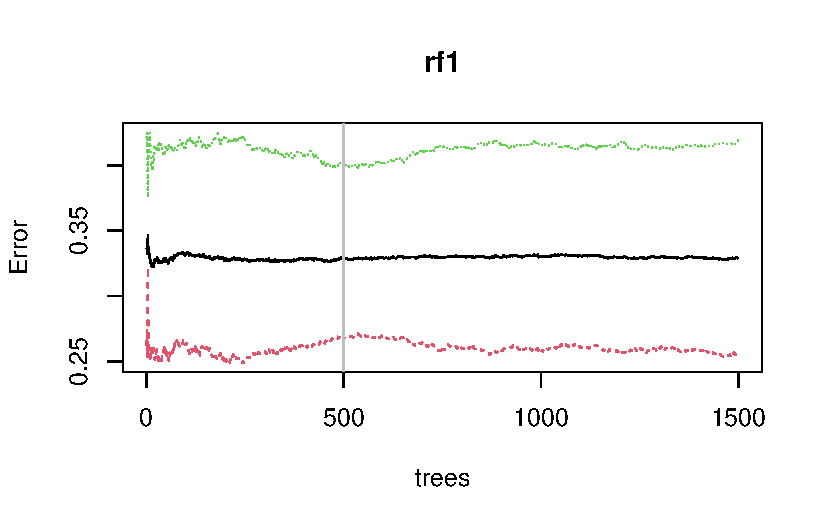
\includegraphics{./randomForest_files/figure-pdf/unnamed-chunk-8-1.pdf}

}

\end{figure}

Vi kan justere resultatet med å endre antall variable som tas med i hver
split (i hvert tre). I forrige eksempel valgte funksjonen å bruke kun to
variable, men det kan settes til f.eks. fire. Merk at det er et poeng at
det ikke skal være så mange variable i hver split! Dette endrer normalt
ikke resultatene veldig mye.

\begin{Shaded}
\begin{Highlighting}[]
\FunctionTok{set.seed}\NormalTok{(}\DecValTok{4356}\NormalTok{)}
\NormalTok{rf2 }\OtherTok{\textless{}{-}} \FunctionTok{randomForest}\NormalTok{(Two\_yr\_Recidivism }\SpecialCharTok{\textasciitilde{}}\NormalTok{ . , }
                    \AttributeTok{mtry=}\DecValTok{4}\NormalTok{,}
                    \AttributeTok{data =}\NormalTok{ compas)}
\NormalTok{rf2}
\end{Highlighting}
\end{Shaded}

\begin{verbatim}

Call:
 randomForest(formula = Two_yr_Recidivism ~ ., data = compas,      mtry = 4) 
               Type of random forest: classification
                     Number of trees: 500
No. of variables tried at each split: 4

        OOB estimate of  error rate: 34.36%
Confusion matrix:
     0    1 class.error
0 2608  755   0.2245019
1 1366 1443   0.4862941
\end{verbatim}

\hypertarget{variable-importance}{%
\subsection{Variable importance}\label{variable-importance}}

For å få ut variable importance må dette settes i estimeringen med
\texttt{importance\ =\ TRUE}. Det tar nå litt lengre tid å estimere, så
med store datasett bør du vente med dette til du ellers er fornøyd med
modellen.

\begin{Shaded}
\begin{Highlighting}[]
\FunctionTok{set.seed}\NormalTok{(}\DecValTok{4356}\NormalTok{)}
\NormalTok{rf }\OtherTok{\textless{}{-}} \FunctionTok{randomForest}\NormalTok{(Two\_yr\_Recidivism }\SpecialCharTok{\textasciitilde{}}\NormalTok{ . , }
                   \AttributeTok{importance =} \ConstantTok{TRUE}\NormalTok{, }
                    \AttributeTok{data =}\NormalTok{ compas)}
\NormalTok{rf}
\end{Highlighting}
\end{Shaded}

\begin{verbatim}

Call:
 randomForest(formula = Two_yr_Recidivism ~ ., data = compas,      importance = TRUE) 
               Type of random forest: classification
                     Number of trees: 500
No. of variables tried at each split: 2

        OOB estimate of  error rate: 32.42%
Confusion matrix:
     0    1 class.error
0 2538  825   0.2453167
1 1176 1633   0.4186543
\end{verbatim}

Vi kan da plotte variable importance plot. Set \texttt{type\ =\ 1} for
at det skal vise gjennomsnittlig reduksjon i accuracy fremfor
gini-koeffisienten. Endring i accuracy er lettest tolkbart og er oftest
mest meningsfult.

\begin{Shaded}
\begin{Highlighting}[]
\FunctionTok{varImpPlot}\NormalTok{(rf, }\AttributeTok{type =} \DecValTok{1}\NormalTok{)}
\end{Highlighting}
\end{Shaded}

\begin{figure}[H]

{\centering 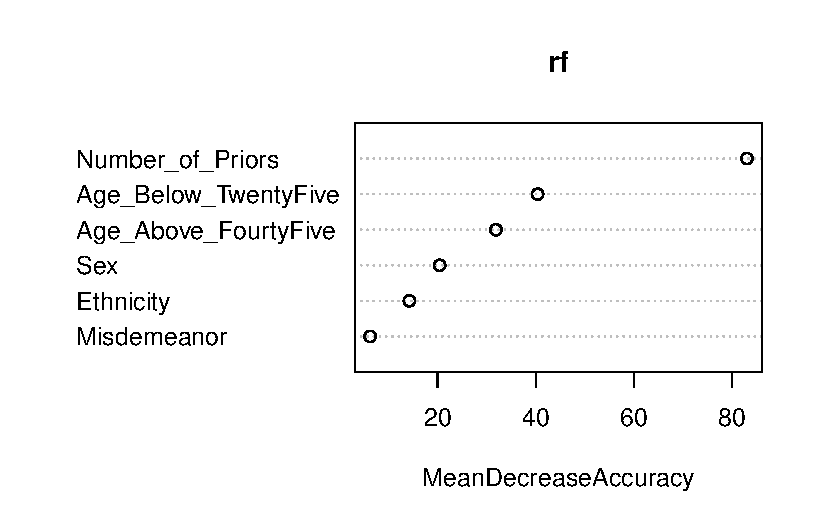
\includegraphics{./randomForest_files/figure-pdf/unnamed-chunk-11-1.pdf}

}

\end{figure}

Her er det altså antall tidligere dommer som har størst betydning for
prediksjon av tilbakefall, etterfulgt av alder og kjønn, og til sist om
lovbruddet var en forseelse eller ikke.\footnote{I norsk straffelov var
  det et skille mellom forseelse og forbrytelse frem til 2015, og dette
  skillet finnes ikke lengre i norsk straffelov. Men med ``forseelse''
  menes det jo i denne sammenheng de mindre alvorlige lovbruddene.}

\hypertarget{partial-dependence}{%
\subsection{Partial dependence}\label{partial-dependence}}

Her må du velge hvilken variabel du ønsker å se på. Det er oftest de
``viktigste variablene'' fra variable importanc som er mest relevante å
se på.

\begin{Shaded}
\begin{Highlighting}[]
\FunctionTok{partialPlot}\NormalTok{(rf, }\AttributeTok{pred.data =}\NormalTok{ compas, }
            \AttributeTok{x.var =}\NormalTok{ Number\_of\_Priors, }
            \AttributeTok{which.class =} \StringTok{"1"}\NormalTok{)}
\end{Highlighting}
\end{Shaded}

\begin{figure}[H]

{\centering 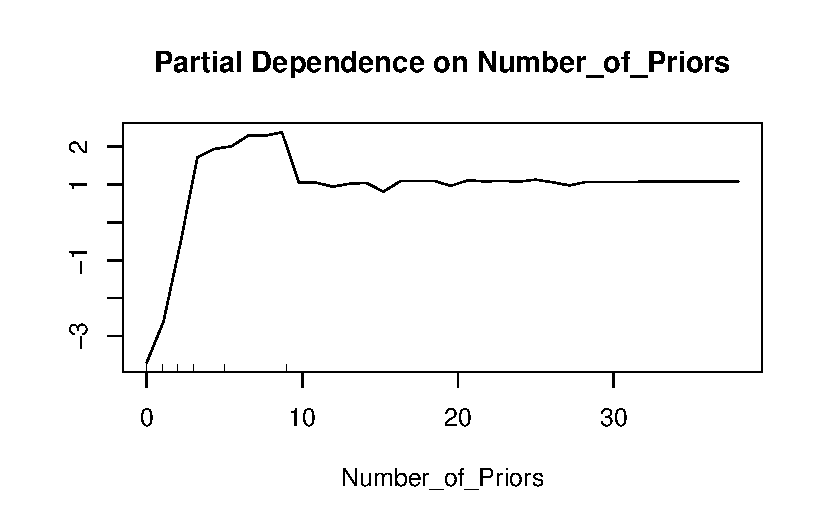
\includegraphics{./randomForest_files/figure-pdf/unnamed-chunk-12-1.pdf}

}

\end{figure}

\hypertarget{tuning-av-random-forest}{%
\section{Tuning av random forest}\label{tuning-av-random-forest}}

Det som faktisk endrer resultatene en god del er sampling prosedyren,
altså hvor mange observasjoner som trekkes til å bygge hvert tre. I
utgangspunktet trekkes 70\% av hele utvalget. Men ved å bruke argumentet
\texttt{sampsize\ =\ ...} kan vi angi en annen andel. Hvis vi angir to
tall er det \emph{antallet} som trekkes fra hver kategori i
utfallsvariabelen. Vi kan altså angi hvor mange som trekkes av de med og
uten tilbakefall, men disse tallene bør ikke settes større enn 70\% av
hver kategori. I disse dataene er det 2809 med tilbakefall og 3364 uten
tilbakefall. Vi kan da velge å trekke maks 1900 fra gruppen med
tilbakefall.

Hensikten med å gjøre dette er at hvis det er et mindretall som har
tilbakefall, så blir hvert tre bygget med mer informasjon om
ikke-residivistene enn residivistene. Hvis vi vekter opp residivistene,
så får disse større inflytelse på hvert tre. Dermed vil dette også
påvirke resultatet. Det er imidlertid vanskelig å vite helt sikkert
hvordan det vil slå ut, så man må prøve seg litt frem. Noen ganger vil
man veie gruppene likt, andre ganger ulikt. Her er et eksempel der de
veies likt:

\begin{Shaded}
\begin{Highlighting}[]
\FunctionTok{set.seed}\NormalTok{(}\DecValTok{4356}\NormalTok{)}
\NormalTok{rf3 }\OtherTok{\textless{}{-}} \FunctionTok{randomForest}\NormalTok{(Two\_yr\_Recidivism }\SpecialCharTok{\textasciitilde{}}\NormalTok{ . , }
                    \AttributeTok{sampsize =} \FunctionTok{c}\NormalTok{(}\DecValTok{1900}\NormalTok{, }\DecValTok{1900}\NormalTok{),}
                    \AttributeTok{data =}\NormalTok{ compas)}
\NormalTok{rf3}
\end{Highlighting}
\end{Shaded}

\begin{verbatim}

Call:
 randomForest(formula = Two_yr_Recidivism ~ ., data = compas,      sampsize = c(1900, 1900)) 
               Type of random forest: classification
                     Number of trees: 500
No. of variables tried at each split: 2

        OOB estimate of  error rate: 32.73%
Confusion matrix:
     0    1 class.error
0 2321 1042   0.3098424
1  978 1831   0.3481666
\end{verbatim}

Her er et eksempel der de veies ulikt:

\begin{Shaded}
\begin{Highlighting}[]
\FunctionTok{set.seed}\NormalTok{(}\DecValTok{4356}\NormalTok{)}
\NormalTok{rf3 }\OtherTok{\textless{}{-}} \FunctionTok{randomForest}\NormalTok{(Two\_yr\_Recidivism }\SpecialCharTok{\textasciitilde{}}\NormalTok{ . , }
                    \AttributeTok{sampsize =} \FunctionTok{c}\NormalTok{(}\DecValTok{1000}\NormalTok{, }\DecValTok{1900}\NormalTok{),}
                   \AttributeTok{data =}\NormalTok{ compas)}
\NormalTok{rf3}
\end{Highlighting}
\end{Shaded}

\begin{verbatim}

Call:
 randomForest(formula = Two_yr_Recidivism ~ ., data = compas,      sampsize = c(1000, 1900)) 
               Type of random forest: classification
                     Number of trees: 500
No. of variables tried at each split: 2

        OOB estimate of  error rate: 41.15%
Confusion matrix:
     0    1 class.error
0 1170 2193   0.6520963
1  347 2462   0.1235315
\end{verbatim}

Det viktige nå er at feilratene for falske positive og falske negative
blir vesentlig forskjellig! Det betyr at ved hvordan vi estimerer
modellen kan vi legge sterke føringer på resultatet. Vi bør derfor ta
stilling til \emph{på forhånd} hvilke feilrater vi er villig til å
akseptere - og hvorvidt de to typer feil er like ille eller ikke. Det er
dette Berk (2016) kaller \emph{asymetriske kostnader} og må vurderes i
henhold til konsekvenser av hva prediksjonen skal brukes til.

Predikere for nye data:

\begin{Shaded}
\begin{Highlighting}[]
\NormalTok{compas\_p }\OtherTok{\textless{}{-}}\NormalTok{ compas }\SpecialCharTok{\%\textgreater{}\%} 
  \FunctionTok{mutate}\NormalTok{(}\AttributeTok{pred\_rf =} \FunctionTok{predict}\NormalTok{(rf, }\AttributeTok{newdata=}\NormalTok{compas))}
\end{Highlighting}
\end{Shaded}

Confusion matrix:

\begin{Shaded}
\begin{Highlighting}[]
\FunctionTok{confusionMatrix}\NormalTok{(compas\_p}\SpecialCharTok{$}\NormalTok{pred\_rf, compas\_p}\SpecialCharTok{$}\NormalTok{Two\_yr\_Recidivism, }\AttributeTok{positive=}\StringTok{"1"}\NormalTok{)}
\end{Highlighting}
\end{Shaded}

\begin{verbatim}
Confusion Matrix and Statistics

          Reference
Prediction    0    1
         0 2595 1156
         1  768 1653
                                          
               Accuracy : 0.6883          
                 95% CI : (0.6765, 0.6998)
    No Information Rate : 0.5449          
    P-Value [Acc > NIR] : < 2.2e-16       
                                          
                  Kappa : 0.3642          
                                          
 Mcnemar's Test P-Value : < 2.2e-16       
                                          
            Sensitivity : 0.5885          
            Specificity : 0.7716          
         Pos Pred Value : 0.6828          
         Neg Pred Value : 0.6918          
             Prevalence : 0.4551          
         Detection Rate : 0.2678          
   Detection Prevalence : 0.3923          
      Balanced Accuracy : 0.6800          
                                          
       'Positive' Class : 1               
                                          
\end{verbatim}

\hypertarget{oppgaver-5}{%
\section{Oppgaver}\label{oppgaver-5}}

\leavevmode\vadjust pre{\hypertarget{exr-}{}}%
\begin{exercise}[]\label{exr-}

Bruk datasettet credit som i forrige oppgave.

\begin{enumerate}
\def\labelenumi{\alph{enumi})}
\tightlist
\item
  Bruk random forest til å gjøre en tilsvarende klassifisering som du
  gjorde med klassifikasjonstre. Bruk default instillinger i
  randomForest().
\item
  Bruk predict() til å klassifisere
\item
  Lag en confusion matrix med table() og gjenta med confusionMatrix()
\item
  Gjør en vurdering av resultatet og sammenlign med resultat fra
  klassifikasjonstre
\end{enumerate}

\end{exercise}

\leavevmode\vadjust pre{\hypertarget{exr-}{}}%
\begin{exercise}[]\label{exr-}

Gjenta oppgave 1, men se om du kan justere modellen til et mer
tilfredsstillende resultat. Gjør deg først opp en mening om hvordan du
vil at confusion matrix skal se ut (f.eks. cost-ratio) og prøv å nærme
deg dette. Bruk parameterne sampsize, mtry og ntree.

\end{exercise}

\leavevmode\vadjust pre{\hypertarget{exr-}{}}%
\begin{exercise}[]\label{exr-}

Tolk random forest a) Hvilke variable har størst prediktiv verdi? Lag et
variable importance plot og gi en tolkning. a) Velg noen av variablene
(gjerne f.eks. de med størst prediktiv verdi) og lag partial dependence
plot.

\end{exercise}

\leavevmode\vadjust pre{\hypertarget{exr-}{}}%
\begin{exercise}[]\label{exr-}

Datafilen credit\_kunder.csv inneholder data om to lånesøkere: Ola
Normann og Kari Hansen. Skal banken gi dem lån? Bruk foretrukne modell
fra forrige oppgave. Hvis du virkelig vil at begge skal få lån kan du
kanskje justere modellen? Legge til/fjerne variable fra formelen og
justere tuning parametrene. Prøv deg frem.

\end{exercise}

\bookmarksetup{startatroot}

\hypertarget{fairness}{%
\chapter{Fairness}\label{fairness}}

\hypertarget{introduksjon-til-fairness}{%
\section{Introduksjon til fairness}\label{introduksjon-til-fairness}}

\begin{Shaded}
\begin{Highlighting}[]
\FunctionTok{library}\NormalTok{(tidyverse)}
\FunctionTok{library}\NormalTok{(randomForest)}
\FunctionTok{library}\NormalTok{(caret)}
\FunctionTok{library}\NormalTok{(fairness)}
\end{Highlighting}
\end{Shaded}

Compas er et risikoverktøy brukt av amerikansk politi i flere stater som
benyttes på individnivå. Bruken av dette verktøyet har vært
kontroversielt i flere år og kraftig kritisert av flere. En viktig grunn
er at prediksjonene slår forskjellig ut for ulike grupper og er slik
sett ``biased'' mot bl.a. svarte borgere. Resultatet er at de blir mer
utsatt for politiets oppmerksomhet enn andre.\footnote{Det er verd å
  minne på at politi i USA i stor grad er mer hardhendte enn norsk
  politi. Konsekvensene er altså litt mer alvorlig enn at unødig mange
  føler seg unødig mistenkte.} Et datasett er gjort tilgjengelig av
\href{https://www.propublica.org/datastore/dataset/compas-recidivism-risk-score-data-and-analysis}{Propublica
her} som vi skal bruke.

\begin{Shaded}
\begin{Highlighting}[]
\NormalTok{compas }\OtherTok{\textless{}{-}} \FunctionTok{readRDS}\NormalTok{(}\StringTok{"../data/compas.rds"}\NormalTok{)}

\FunctionTok{glimpse}\NormalTok{(compas)}
\end{Highlighting}
\end{Shaded}

\begin{verbatim}
Rows: 6,172
Columns: 7
$ Two_yr_Recidivism    <fct> 0, 1, 1, 0, 1, 0, 0, 0, 1, 0, 0, 1, 1, 0, 0, 1, 1~
$ Number_of_Priors     <int> 0, 0, 4, 0, 14, 3, 0, 0, 3, 0, 0, 1, 7, 0, 3, 6, ~
$ Age_Above_FourtyFive <fct> 1, 0, 0, 0, 0, 0, 0, 0, 0, 0, 0, 1, 0, 0, 0, 0, 0~
$ Age_Below_TwentyFive <fct> 0, 0, 1, 0, 0, 0, 0, 0, 1, 0, 0, 0, 0, 0, 0, 0, 0~
$ Misdemeanor          <fct> 0, 0, 0, 1, 0, 0, 1, 0, 1, 1, 0, 0, 0, 1, 0, 0, 0~
$ Ethnicity            <fct> Other, African_American, African_American, Other,~
$ Sex                  <fct> Male, Male, Male, Male, Male, Male, Female, Male,~
\end{verbatim}

Vi tilpasser først en random forest modell.

\begin{Shaded}
\begin{Highlighting}[]
\FunctionTok{set.seed}\NormalTok{(}\DecValTok{4356}\NormalTok{)}
\FunctionTok{glimpse}\NormalTok{(compas)}
\end{Highlighting}
\end{Shaded}

\begin{verbatim}
Rows: 6,172
Columns: 7
$ Two_yr_Recidivism    <fct> 0, 1, 1, 0, 1, 0, 0, 0, 1, 0, 0, 1, 1, 0, 0, 1, 1~
$ Number_of_Priors     <int> 0, 0, 4, 0, 14, 3, 0, 0, 3, 0, 0, 1, 7, 0, 3, 6, ~
$ Age_Above_FourtyFive <fct> 1, 0, 0, 0, 0, 0, 0, 0, 0, 0, 0, 1, 0, 0, 0, 0, 0~
$ Age_Below_TwentyFive <fct> 0, 0, 1, 0, 0, 0, 0, 0, 1, 0, 0, 0, 0, 0, 0, 0, 0~
$ Misdemeanor          <fct> 0, 0, 0, 1, 0, 0, 1, 0, 1, 1, 0, 0, 0, 1, 0, 0, 0~
$ Ethnicity            <fct> Other, African_American, African_American, Other,~
$ Sex                  <fct> Male, Male, Male, Male, Male, Male, Female, Male,~
\end{verbatim}

\begin{Shaded}
\begin{Highlighting}[]
\NormalTok{rf }\OtherTok{\textless{}{-}} \FunctionTok{randomForest}\NormalTok{(Two\_yr\_Recidivism }\SpecialCharTok{\textasciitilde{}}\NormalTok{ .,}
                   \CommentTok{\#importance = TRUE,}
                    \AttributeTok{data =}\NormalTok{ compas)}
\end{Highlighting}
\end{Shaded}

Lager en prediksjon i nytt datasett

\begin{Shaded}
\begin{Highlighting}[]
\NormalTok{compas\_p }\OtherTok{\textless{}{-}}\NormalTok{ compas }\SpecialCharTok{\%\textgreater{}\%} 
  \FunctionTok{mutate}\NormalTok{(}\AttributeTok{pred\_rf =} \FunctionTok{predict}\NormalTok{(rf))  }
\end{Highlighting}
\end{Shaded}

Confusion matrix

\begin{Shaded}
\begin{Highlighting}[]
\FunctionTok{confusionMatrix}\NormalTok{(compas\_p}\SpecialCharTok{$}\NormalTok{pred\_rf,}
\NormalTok{                compas\_p}\SpecialCharTok{$}\NormalTok{Two\_yr\_Recidivism, }\AttributeTok{positive=}\StringTok{"1"}\NormalTok{)}
\end{Highlighting}
\end{Shaded}

\begin{verbatim}
Confusion Matrix and Statistics

          Reference
Prediction    0    1
         0 2462 1132
         1  901 1677
                                          
               Accuracy : 0.6706          
                 95% CI : (0.6587, 0.6823)
    No Information Rate : 0.5449          
    P-Value [Acc > NIR] : < 2.2e-16       
                                          
                  Kappa : 0.3313          
                                          
 Mcnemar's Test P-Value : 3.378e-07       
                                          
            Sensitivity : 0.5970          
            Specificity : 0.7321          
         Pos Pred Value : 0.6505          
         Neg Pred Value : 0.6850          
             Prevalence : 0.4551          
         Detection Rate : 0.2717          
   Detection Prevalence : 0.4177          
      Balanced Accuracy : 0.6645          
                                          
       'Positive' Class : 1               
                                          
\end{verbatim}

Splitter datasettet i to etter kjønn. Her for menn.

\begin{Shaded}
\begin{Highlighting}[]
\NormalTok{compas\_1 }\OtherTok{\textless{}{-}}\NormalTok{ compas\_p }\SpecialCharTok{\%\textgreater{}\%} 
  \FunctionTok{filter}\NormalTok{(Sex }\SpecialCharTok{==} \StringTok{"Male"}\NormalTok{)}
\end{Highlighting}
\end{Shaded}

Confusion matrix for menn

\begin{Shaded}
\begin{Highlighting}[]
\FunctionTok{confusionMatrix}\NormalTok{(compas\_1}\SpecialCharTok{$}\NormalTok{pred\_rf,}
\NormalTok{                compas\_1}\SpecialCharTok{$}\NormalTok{Two\_yr\_Recidivism, }\AttributeTok{positive=}\StringTok{"1"}\NormalTok{)}
\end{Highlighting}
\end{Shaded}

\begin{verbatim}
Confusion Matrix and Statistics

          Reference
Prediction    0    1
         0 1807  897
         1  794 1499
                                          
               Accuracy : 0.6616          
                 95% CI : (0.6483, 0.6747)
    No Information Rate : 0.5205          
    P-Value [Acc > NIR] : < 2e-16         
                                          
                  Kappa : 0.3209          
                                          
 Mcnemar's Test P-Value : 0.01312         
                                          
            Sensitivity : 0.6256          
            Specificity : 0.6947          
         Pos Pred Value : 0.6537          
         Neg Pred Value : 0.6683          
             Prevalence : 0.4795          
         Detection Rate : 0.3000          
   Detection Prevalence : 0.4589          
      Balanced Accuracy : 0.6602          
                                          
       'Positive' Class : 1               
                                          
\end{verbatim}

Splitter datasettet i to etter kjønn. Her for kvinner.

\begin{Shaded}
\begin{Highlighting}[]
\NormalTok{compas\_2 }\OtherTok{\textless{}{-}}\NormalTok{ compas\_p }\SpecialCharTok{\%\textgreater{}\%} 
  \FunctionTok{filter}\NormalTok{(Sex }\SpecialCharTok{==} \StringTok{"Female"}\NormalTok{)}
\end{Highlighting}
\end{Shaded}

Confusion matrix for kvinner

\begin{Shaded}
\begin{Highlighting}[]
\FunctionTok{confusionMatrix}\NormalTok{(compas\_2}\SpecialCharTok{$}\NormalTok{pred\_rf,}
\NormalTok{                compas\_2}\SpecialCharTok{$}\NormalTok{Two\_yr\_Recidivism, }\AttributeTok{positive=}\StringTok{"1"}\NormalTok{)}
\end{Highlighting}
\end{Shaded}

\begin{verbatim}
Confusion Matrix and Statistics

          Reference
Prediction   0   1
         0 655 235
         1 107 178
                                         
               Accuracy : 0.7089         
                 95% CI : (0.682, 0.7348)
    No Information Rate : 0.6485         
    P-Value [Acc > NIR] : 6.251e-06      
                                         
                  Kappa : 0.3128         
                                         
 Mcnemar's Test P-Value : 6.539e-12      
                                         
            Sensitivity : 0.4310         
            Specificity : 0.8596         
         Pos Pred Value : 0.6246         
         Neg Pred Value : 0.7360         
             Prevalence : 0.3515         
         Detection Rate : 0.1515         
   Detection Prevalence : 0.2426         
      Balanced Accuracy : 0.6453         
                                         
       'Positive' Class : 1              
                                         
\end{verbatim}

Bruker funksjoner i fairness-pakken til å gjøre det samme:

\begin{Shaded}
\begin{Highlighting}[]
\NormalTok{acc }\OtherTok{\textless{}{-}} \FunctionTok{acc\_parity}\NormalTok{(}\AttributeTok{data =}\NormalTok{ compas\_p, }
                  \AttributeTok{outcome      =} \StringTok{\textquotesingle{}Two\_yr\_Recidivism\textquotesingle{}}\NormalTok{, }
                  \AttributeTok{group        =} \StringTok{\textquotesingle{}Sex\textquotesingle{}}\NormalTok{,}
                  \AttributeTok{preds        =} \StringTok{\textquotesingle{}pred\_rf\textquotesingle{}}\NormalTok{, }
                  \AttributeTok{base         =} \StringTok{\textquotesingle{}Female\textquotesingle{}}\NormalTok{)}
\NormalTok{acc}\SpecialCharTok{$}\NormalTok{Metric}
\end{Highlighting}
\end{Shaded}

\begin{verbatim}
                      Female        Male
Accuracy           0.7089362    0.661597
Accuracy Parity    1.0000000    0.933225
Group size      1175.0000000 4997.000000
\end{verbatim}

Her er en grafisk fremstilling av ACC

\begin{Shaded}
\begin{Highlighting}[]
\NormalTok{acc}\SpecialCharTok{$}\NormalTok{Metric\_plot}
\end{Highlighting}
\end{Shaded}

\begin{figure}[H]

{\centering 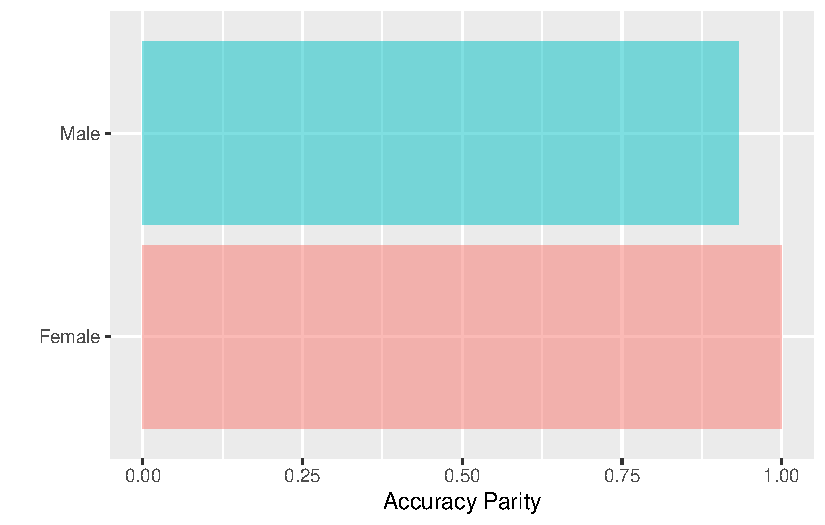
\includegraphics{./fairness_files/figure-pdf/unnamed-chunk-11-1.pdf}

}

\end{figure}

\hypertarget{flere-muxe5l-puxe5-fairness}{%
\section{Flere mål på fairness}\label{flere-muxe5l-puxe5-fairness}}

\hypertarget{tuning-til-mer-fairness}{%
\section{Tuning til mer fairness}\label{tuning-til-mer-fairness}}

\hypertarget{oppgaver-6}{%
\section{Oppgaver}\label{oppgaver-6}}

\bookmarksetup{startatroot}

\hypertarget{boosting}{%
\chapter{Boosting}\label{boosting}}

Det er flere typer boosting-algoritmer. Vi skal først se på adaptive
boosting fordi det er den enkleste (og eldste) varianten. Deretter ser
vi på gradient boosting fordi andre mer avanserte boosting-algoritmer er
varianter av denne.

Kilde:
https://towardsdatascience.com/how-to-select-between-boosting-algorithm-e8d1b15924f7

\hypertarget{adaptive-boosting---adaboost}{%
\section{Adaptive boosting -
Adaboost}\label{adaptive-boosting---adaboost}}

Adaptive boosting har et enkelt prinsipp: Først estimeres en modell, og
deretter estimeres en ny modell der feilklassifikasjonene fra forrige
modell vektes tyngre. Teorien tilsier at dette vil bedre
klassifikasjonen. Så fortsetter den slik og estimerer nye vektede
modeller til vi ikke får noen vesetnlig forbedring.

\hypertarget{gradient-boosting---gbm}{%
\section{Gradient boosting - gbm}\label{gradient-boosting---gbm}}

Gradient boosting er bygget på et tilsvarende prinsipp, men vekter ikke
dataene. Derimot bruker den loss-funksjon i stedet.

\hypertarget{extreme-gradient-boosting---xgboost}{%
\section{Extreme gradient boosting -
XGboost}\label{extreme-gradient-boosting---xgboost}}

\bookmarksetup{startatroot}

\hypertarget{unsupervised-learning}{%
\chapter{Unsupervised learning}\label{unsupervised-learning}}

\begin{Shaded}
\begin{Highlighting}[]
\FunctionTok{library}\NormalTok{(tidyverse)}
\end{Highlighting}
\end{Shaded}

\begin{verbatim}
-- Attaching packages --------------------------------------- tidyverse 1.3.2 --
v ggplot2 3.4.0      v purrr   0.3.5 
v tibble  3.1.8      v dplyr   1.0.10
v tidyr   1.2.1      v stringr 1.4.1 
v readr   2.1.3      v forcats 0.5.2 
-- Conflicts ------------------------------------------ tidyverse_conflicts() --
x dplyr::filter() masks stats::filter()
x dplyr::lag()    masks stats::lag()
\end{verbatim}

\begin{Shaded}
\begin{Highlighting}[]
\FunctionTok{library}\NormalTok{(dendextend)}
\end{Highlighting}
\end{Shaded}

\begin{verbatim}

---------------------
Welcome to dendextend version 1.16.0
Type citation('dendextend') for how to cite the package.

Type browseVignettes(package = 'dendextend') for the package vignette.
The github page is: https://github.com/talgalili/dendextend/

Suggestions and bug-reports can be submitted at: https://github.com/talgalili/dendextend/issues
You may ask questions at stackoverflow, use the r and dendextend tags: 
     https://stackoverflow.com/questions/tagged/dendextend

    To suppress this message use:  suppressPackageStartupMessages(library(dendextend))
---------------------


Attaching package: 'dendextend'

The following object is masked from 'package:stats':

    cutree
\end{verbatim}

\begin{Shaded}
\begin{Highlighting}[]
\FunctionTok{library}\NormalTok{(directlabels)}
\end{Highlighting}
\end{Shaded}

\hypertarget{hierarkisk-klustering}{%
\section{Hierarkisk klustering}\label{hierarkisk-klustering}}

\leavevmode\vadjust pre{\hypertarget{exr-}{}}%
\begin{exercise}[]\label{exr-}

Last ned filen krim2016.RData fra Canvas. Dette er deler av dataene vi
brukte i første seminar med kommunetall. Her er det anmeldt kriminalitet
per 1000 innbyggere i kommuner i 2016.

\begin{enumerate}
\def\labelenumi{\alph{enumi})}
\tightlist
\item
  Gjør en hierarkisk klusteranalsyse. Er det noen kommuner som skiller
  seg veldig fra de andre? Spiller det noen rolle hvilken type distance
  du setter?
\item
  Hvilke kommuner er de de klusterne som skiller seg ut?
\item
  Hva kjennetegner lovbruddsbildet i de ulike klustrene? Kan du tenke
  deg noen grunner til at akkurat disse stikker seg ut?
\end{enumerate}

\end{exercise}

\begin{solution}

Leser inn data om inntektsutvikling for ulike yrker fra 2001 til 2016

Dataene er i ``bred'' format. Det er slik vi vil ha det for
clusteranalyse, men dårlig for å lage en graf.

\begin{Shaded}
\begin{Highlighting}[]
\FunctionTok{load}\NormalTok{(}\StringTok{"../data/oes.RData"}\NormalTok{)}

\NormalTok{gathered\_oes }\OtherTok{\textless{}{-}} \FunctionTok{gather}\NormalTok{(}\AttributeTok{data =}\NormalTok{ df\_oes, }
                       \AttributeTok{key =}\NormalTok{ year, }
                       \AttributeTok{value =}\NormalTok{ mean\_salary, }
                       \SpecialCharTok{{-}}\NormalTok{occupation)}

\FunctionTok{ggplot}\NormalTok{(gathered\_oes, }\FunctionTok{aes}\NormalTok{(}\AttributeTok{x=}\FunctionTok{as.numeric}\NormalTok{(year), }\AttributeTok{y=}\NormalTok{mean\_salary, }\AttributeTok{col =}\NormalTok{ occupation))}\SpecialCharTok{+}
  \FunctionTok{geom\_line}\NormalTok{()}
\end{Highlighting}
\end{Shaded}

\begin{figure}[H]

{\centering \includegraphics{./unsupervised_files/figure-pdf/unnamed-chunk-2-1.pdf}

}

\end{figure}

\begin{Shaded}
\begin{Highlighting}[]
\NormalTok{dist\_oes }\OtherTok{\textless{}{-}} \FunctionTok{dist}\NormalTok{(df\_oes[,}\SpecialCharTok{{-}}\DecValTok{1}\NormalTok{], }\AttributeTok{method =} \StringTok{"euclidian"}\NormalTok{) }\CommentTok{\# calculate distances }

\NormalTok{hc\_oes }\OtherTok{\textless{}{-}} \FunctionTok{hclust}\NormalTok{(dist\_oes, }\AttributeTok{method =} \StringTok{"single"}\NormalTok{)  }\CommentTok{\# minste avstand}

\NormalTok{hc\_oes }\OtherTok{\textless{}{-}} \FunctionTok{hclust}\NormalTok{(dist\_oes, }\AttributeTok{method =} \StringTok{"complete"}\NormalTok{) }\CommentTok{\# lengste avstand}

\NormalTok{hc\_oes }\OtherTok{\textless{}{-}} \FunctionTok{hclust}\NormalTok{(dist\_oes, }\AttributeTok{method =} \StringTok{"average"}\NormalTok{) }\CommentTok{\#gjennomsnittlig avstand}

\FunctionTok{par}\NormalTok{(}\AttributeTok{mar=}\FunctionTok{c}\NormalTok{(}\DecValTok{10}\NormalTok{,}\DecValTok{4}\NormalTok{,}\DecValTok{2}\NormalTok{,}\DecValTok{2}\NormalTok{))  }\CommentTok{\# Endre marginer for base{-}plot}

\NormalTok{dend\_oes }\OtherTok{\textless{}{-}} \FunctionTok{as.dendrogram}\NormalTok{(hc\_oes) }\CommentTok{\#Create a dendrogram object}
\NormalTok{dend\_colored }\OtherTok{\textless{}{-}} \FunctionTok{color\_branches}\NormalTok{(dend\_oes, }\AttributeTok{h =} \DecValTok{100000}\NormalTok{)}
\FunctionTok{plot}\NormalTok{(dend\_colored)}

\CommentTok{\# Illustrer mulige cutoff {-} legger linjer oppå eksisterende plot}
\FunctionTok{abline}\NormalTok{(}\AttributeTok{h=}\DecValTok{100000}\NormalTok{, }\AttributeTok{col=}\StringTok{"red"}\NormalTok{, }\AttributeTok{lwd=}\FloatTok{1.5}\NormalTok{)  }\CommentTok{\# Viser cut ved h=100000}
\FunctionTok{abline}\NormalTok{(}\AttributeTok{h=}\DecValTok{10000}\NormalTok{, }\AttributeTok{col=}\StringTok{"red"}\NormalTok{, }\AttributeTok{lwd=}\FloatTok{1.5}\NormalTok{)   }\CommentTok{\# Viser cut ved h=10000}
\end{Highlighting}
\end{Shaded}

\begin{figure}[H]

{\centering 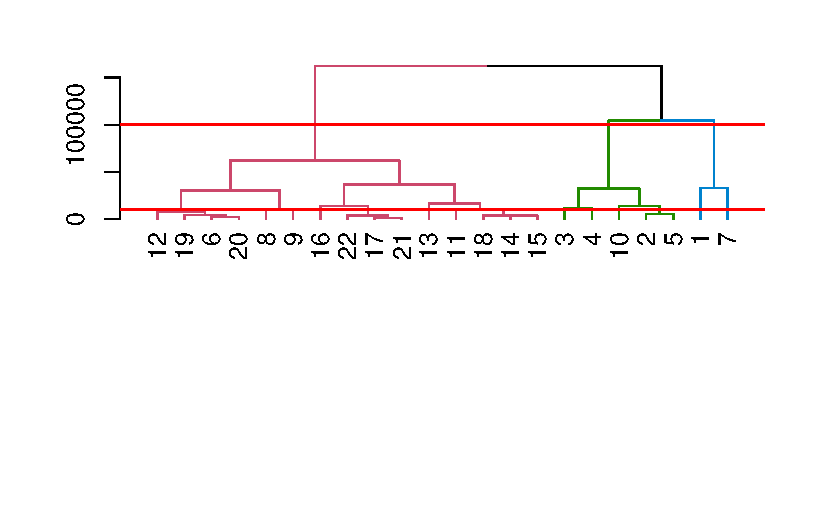
\includegraphics{./unsupervised_files/figure-pdf/unnamed-chunk-2-2.pdf}

}

\end{figure}

\begin{Shaded}
\begin{Highlighting}[]
\CommentTok{\# Henter ut cluster ved valgt h}
\NormalTok{cluster }\OtherTok{\textless{}{-}} \FunctionTok{cutree}\NormalTok{(hc\_oes, }\AttributeTok{h=}\DecValTok{100000}\NormalTok{)}
\CommentTok{\#cluster \textless{}{-} cutree(hc\_oes, k=3)}
\FunctionTok{table}\NormalTok{(cluster)}
\end{Highlighting}
\end{Shaded}

\begin{verbatim}
cluster
 1  2  3 
 2  5 15 
\end{verbatim}

\begin{Shaded}
\begin{Highlighting}[]
\CommentTok{\# Legger til vektoren cluster til opprinnelige data}
\NormalTok{hclust\_oes }\OtherTok{\textless{}{-}} \FunctionTok{mutate}\NormalTok{(df\_oes, }\AttributeTok{cluster =}\NormalTok{ cluster)}

\FunctionTok{head}\NormalTok{(hclust\_oes)}
\end{Highlighting}
\end{Shaded}

\begin{verbatim}
                 occupation  2001  2002  2003  2004  2005  2006  2007   2008
1                Management 70800 78870 83400 87090 88450 91930 96150 100310
2       Business Operations 50580 53350 56000 57120 57930 60000 62410  64720
3          Computer Science 60350 61630 64150 66370 67100 69240 72190  74500
4  Architecture/Engineering 56330 58020 60390 63060 63910 66190 68880  71430
5 Life/Physical/Social Sci. 49710 52380 54930 57550 58030 59660 62020  64280
6        Community Services 34190 34630 35800 37050 37530 39000 40540  41790
    2010   2011   2012   2013   2014   2015   2016 cluster
1 105440 107410 108570 110550 112490 115020 118020       1
2  67690  68740  69550  71020  72410  73800  75070       2
3  77230  78730  80180  82010  83970  86170  87880       2
4  75550  77120  79000  80100  81520  82980  84300       2
5  66390  67470  68360  69400  70070  71220  72930       2
6  43180  43830  44240  44710  45310  46160  47200       3
\end{verbatim}

\begin{Shaded}
\begin{Highlighting}[]
\CommentTok{\# vrenger dataene "nedover" for å plotte}
\NormalTok{gathered\_oes }\OtherTok{\textless{}{-}} \FunctionTok{gather}\NormalTok{(}\AttributeTok{data =}\NormalTok{ hclust\_oes,    }\CommentTok{\# datasett}
                       \AttributeTok{key =}\NormalTok{ year,           }\CommentTok{\# navn på ny variabel, verdier hentes fra gamle variabelnavn}
                       \AttributeTok{value =}\NormalTok{ mean\_salary,  }\CommentTok{\# navn på ny variabel med gamle variabelverdier}
                       \SpecialCharTok{{-}}\NormalTok{occupation, }\SpecialCharTok{{-}}\NormalTok{cluster) }\CommentTok{\# variable som skal beholdes / grupperes etter}
\FunctionTok{ggplot}\NormalTok{(gathered\_oes, }\FunctionTok{aes}\NormalTok{(}\AttributeTok{x =}\NormalTok{ year, }\AttributeTok{y =}\NormalTok{ mean\_salary, }\AttributeTok{color =} \FunctionTok{factor}\NormalTok{(cluster), }\AttributeTok{group =}\NormalTok{ occupation)) }\SpecialCharTok{+} 
  \FunctionTok{geom\_line}\NormalTok{()}
\end{Highlighting}
\end{Shaded}

\begin{figure}[H]

{\centering 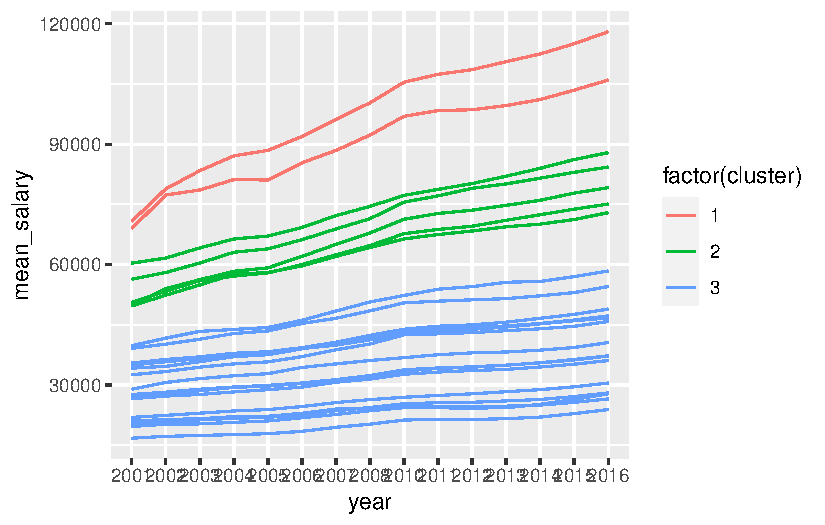
\includegraphics{./unsupervised_files/figure-pdf/unnamed-chunk-2-3.pdf}

}

\end{figure}

\end{solution}

\hypertarget{k-means-klustering}{%
\section{K-means klustering}\label{k-means-klustering}}

\leavevmode\vadjust pre{\hypertarget{exr-}{}}%
\begin{exercise}[]\label{exr-}

Gjenta analysen over med k-means clustering. Hvor mange klustre bør det
være? Får du samme resultat?

\end{exercise}

\begin{solution}

\begin{Shaded}
\begin{Highlighting}[]
\DocumentationTok{\#\# K{-}means clustering med samme data }

\CommentTok{\# Eksempel ved å sette antall kluster til 3}
\CommentTok{\# I dette tilfellet bør vi få samme resultat}
\NormalTok{km\_oes }\OtherTok{\textless{}{-}} \FunctionTok{kmeans}\NormalTok{(dist\_oes, }\AttributeTok{centers =} \DecValTok{3}\NormalTok{)}

\FunctionTok{table}\NormalTok{(km\_oes}\SpecialCharTok{$}\NormalTok{cluster)}
\end{Highlighting}
\end{Shaded}

\begin{verbatim}

1 2 3 
8 7 7 
\end{verbatim}

\begin{Shaded}
\begin{Highlighting}[]
\NormalTok{kmclust\_oes }\OtherTok{\textless{}{-}} \FunctionTok{mutate}\NormalTok{(df\_oes, }\AttributeTok{cluster=}\NormalTok{km\_oes}\SpecialCharTok{$}\NormalTok{cluster)}

\CommentTok{\# Plotter}
\NormalTok{gathered\_kmoes }\OtherTok{\textless{}{-}} \FunctionTok{gather}\NormalTok{(}\AttributeTok{data =}\NormalTok{ kmclust\_oes,    }\CommentTok{\# datasett}
                       \AttributeTok{key =}\NormalTok{ year,           }\CommentTok{\# navn på ny variabel, verdier hentes fra gamle variabelnavn}
                       \AttributeTok{value =}\NormalTok{ mean\_salary,  }\CommentTok{\# navn på ny variabel med gamle variabelverdier}
                       \SpecialCharTok{{-}}\NormalTok{occupation, }\SpecialCharTok{{-}}\NormalTok{cluster) }\CommentTok{\# variable som skal beholdes / grupperes etter}
\FunctionTok{ggplot}\NormalTok{(gathered\_kmoes, }\FunctionTok{aes}\NormalTok{(}\AttributeTok{x =}\NormalTok{ year, }\AttributeTok{y =}\NormalTok{ mean\_salary, }\AttributeTok{color =} \FunctionTok{factor}\NormalTok{(cluster), }\AttributeTok{group =}\NormalTok{ occupation)) }\SpecialCharTok{+} 
  \FunctionTok{geom\_line}\NormalTok{()}
\end{Highlighting}
\end{Shaded}

\begin{figure}[H]

{\centering 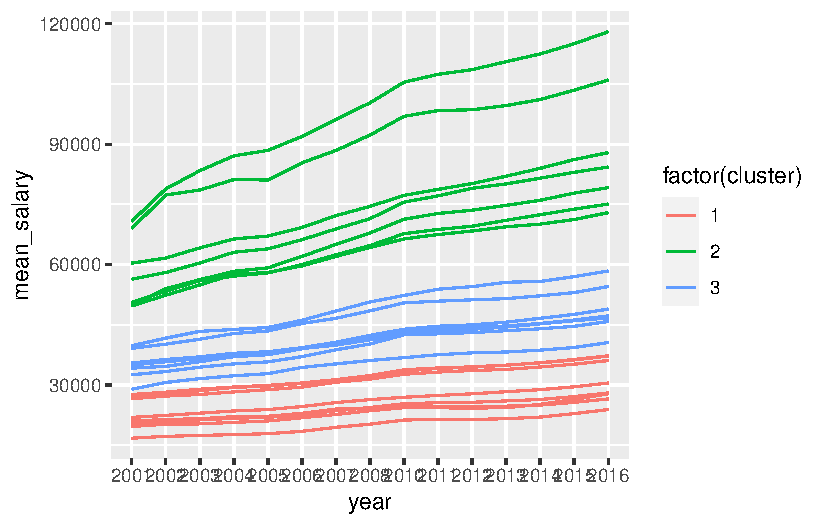
\includegraphics{./unsupervised_files/figure-pdf/unnamed-chunk-3-1.pdf}

}

\end{figure}

\begin{Shaded}
\begin{Highlighting}[]
\DocumentationTok{\#\#\# K{-}means clustering. Make a search}
\NormalTok{wss }\OtherTok{\textless{}{-}} \DecValTok{0}
\CommentTok{\# For 1 to 15 cluster centers}
\ControlFlowTok{for}\NormalTok{ (i }\ControlFlowTok{in} \DecValTok{1}\SpecialCharTok{:}\DecValTok{5}\NormalTok{) \{}
\NormalTok{  km.out }\OtherTok{\textless{}{-}} \FunctionTok{kmeans}\NormalTok{(dist\_oes, }\AttributeTok{centers =}\NormalTok{ i, }\AttributeTok{nstart=}\DecValTok{20}\NormalTok{)}
  \CommentTok{\# Save total within sum of squares to wss variable}
\NormalTok{  wss[i] }\OtherTok{\textless{}{-}}\NormalTok{ km.out}\SpecialCharTok{$}\NormalTok{tot.withinss}
\NormalTok{\}}

\CommentTok{\# Plot total within sum of squares vs. number of clusters}
\FunctionTok{plot}\NormalTok{(}\DecValTok{1}\SpecialCharTok{:}\DecValTok{5}\NormalTok{, wss, }\AttributeTok{type =} \StringTok{"b"}\NormalTok{, }
     \AttributeTok{xlab =} \StringTok{"Number of Clusters"}\NormalTok{, }
     \AttributeTok{ylab =} \StringTok{"Within groups sum of squares"}\NormalTok{)}
\CommentTok{\# Marker "albuen" med en linje i plottet }
\FunctionTok{abline}\NormalTok{(}\AttributeTok{v=}\DecValTok{2}\NormalTok{, }\AttributeTok{col=}\StringTok{"red"}\NormalTok{)}
\end{Highlighting}
\end{Shaded}

\begin{figure}[H]

{\centering 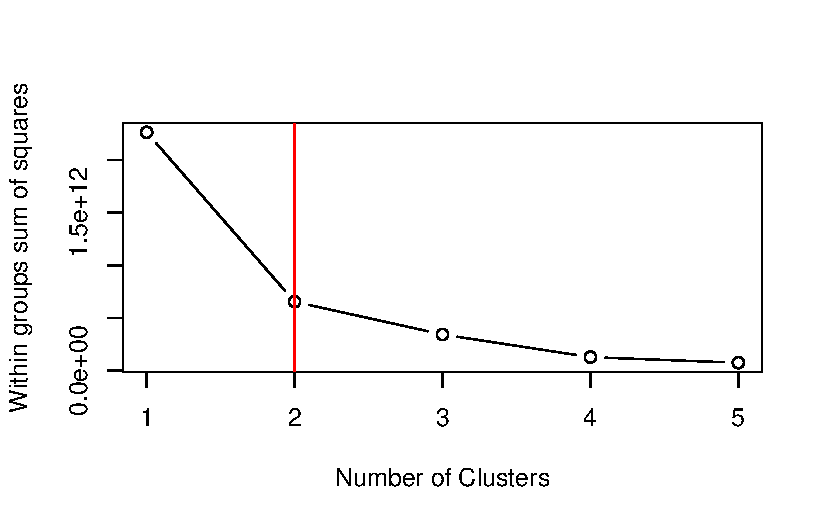
\includegraphics{./unsupervised_files/figure-pdf/unnamed-chunk-3-2.pdf}

}

\end{figure}

\begin{Shaded}
\begin{Highlighting}[]
\NormalTok{oes }\OtherTok{\textless{}{-}} \FunctionTok{readRDS}\NormalTok{(}\StringTok{"../data/oes.rds"}\NormalTok{)}

\DocumentationTok{\#\# Create final clustering}
\NormalTok{km\_oes }\OtherTok{\textless{}{-}} \FunctionTok{kmeans}\NormalTok{(oes, }\AttributeTok{centers =} \DecValTok{2}\NormalTok{, }\AttributeTok{nstart=}\DecValTok{20}\NormalTok{)}
\FunctionTok{table}\NormalTok{(km\_oes}\SpecialCharTok{$}\NormalTok{cluster)}
\end{Highlighting}
\end{Shaded}

\begin{verbatim}

 1  2 
 7 15 
\end{verbatim}

\begin{Shaded}
\begin{Highlighting}[]
\NormalTok{kmclust\_oes }\OtherTok{\textless{}{-}} \FunctionTok{mutate}\NormalTok{(df\_oes, }\AttributeTok{cluster=}\NormalTok{km\_oes}\SpecialCharTok{$}\NormalTok{cluster)}
\NormalTok{gathered\_kmoes }\OtherTok{\textless{}{-}} \FunctionTok{gather}\NormalTok{(}\AttributeTok{data =}\NormalTok{ kmclust\_oes,    }\CommentTok{\# datasett}
                         \AttributeTok{key =}\NormalTok{ year,           }\CommentTok{\# navn på ny variabel, verdier hentes fra gamle variabelnavn}
                         \AttributeTok{value =}\NormalTok{ mean\_salary,  }\CommentTok{\# navn på ny variabel med gamle variabelverdier}
                         \SpecialCharTok{{-}}\NormalTok{occupation, }\SpecialCharTok{{-}}\NormalTok{cluster) }\CommentTok{\# variable som skal beholdes / grupperes etter}
\FunctionTok{ggplot}\NormalTok{(gathered\_kmoes, }\FunctionTok{aes}\NormalTok{(}\AttributeTok{x =}\NormalTok{ year, }\AttributeTok{y =}\NormalTok{ mean\_salary, }\AttributeTok{color =} \FunctionTok{factor}\NormalTok{(cluster), }\AttributeTok{group =}\NormalTok{ occupation)) }\SpecialCharTok{+} 
  \FunctionTok{geom\_line}\NormalTok{()}
\end{Highlighting}
\end{Shaded}

\begin{figure}[H]

{\centering 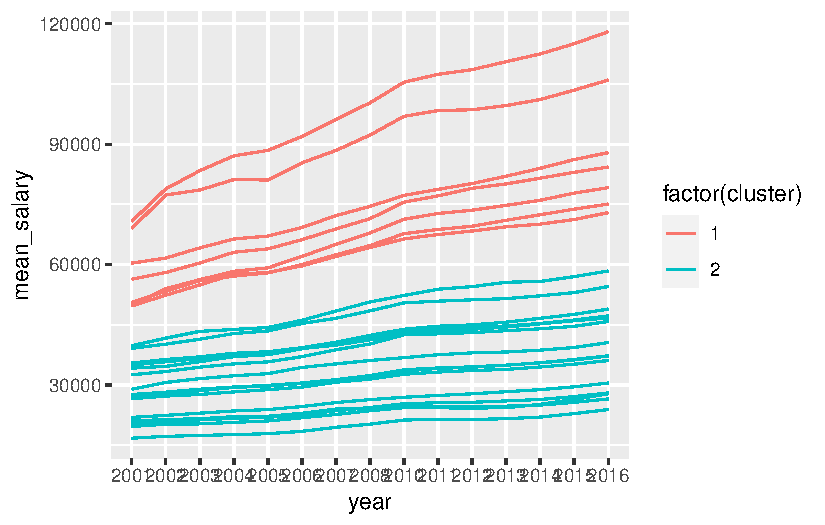
\includegraphics{./unsupervised_files/figure-pdf/unnamed-chunk-3-3.pdf}

}

\end{figure}

\end{solution}

\hypertarget{datareduksjon-med-principal-component-analysis-pca}{%
\section{Datareduksjon med principal component analysis
(PCA)}\label{datareduksjon-med-principal-component-analysis-pca}}

\hypertarget{multippel-korrespondanseanalyse}{%
\subsection{Multippel
korrespondanseanalyse}\label{multippel-korrespondanseanalyse}}

PCA har egentlig som forutsetning av variablene er kontinuerlige, og det
er litt trøblete å bruke det på kategoriske variable. Men ofte har vi
kategoriske variable.

En variant av PCA for kategoriske variable er korrespondanseanalyse, som
i teorien altså skal være bedre enn PCA. I praksis er det imidlertid
ikke nødvendigvis veldig stor forskjell (REF), så det er neppe stor
skade skjedd hvis man bruker PCA likevel.

\bookmarksetup{startatroot}

\hypertarget{references}{%
\chapter*{References}\label{references}}
\addcontentsline{toc}{chapter}{References}

\markboth{References}{References}

\hypertarget{refs}{}
\begin{CSLReferences}{1}{0}
\leavevmode\vadjust pre{\hypertarget{ref-berk2016a}{}}%
Berk, Richard. 2016. \emph{Statistical Learning from a Regression
Perspective}. USA: Springer.

\end{CSLReferences}

\appendix
\addcontentsline{toc}{part}{Appendices}

\hypertarget{datasett}{%
\chapter{Datasett}\label{datasett}}

I de følgende oppgavene kan man bruke ulike datasett og gjøre omtrent de
samme operasjonene. Hvert kapittel innleder med et empirisk eksempel som
illustrerer hvordan det gjøres i R. Det du må finne ut av er hva hver
del av koden gjør utover de ganske korte forklaringene i teksten.

En foreslått arbeidsmåte er da at du først gjør de samme analysene i
eksempelet og sørger for at du skjønner hvordan ting fungerer. Deretter
velger du et annet datasett (av de nedenforstående) og gjør en
tilsvarende analyse på det datasettet. Så kan du fortsette med nye
datasett ettersom hva du har tid til. Å gjøre flere analyser med ulike
datasett er en fin forberedelse til eksamen.

Husk at for hvert datasett er det ulike relevante problemstillinger som
har betydning for hvordan du gjennomfører og tolker resultatet. Du må
derfor ikke ta lett på tekstoppgavene!

I disse oppgavene skal vi bruke flere forskjellige datasett. Last de ned
og legg dem i din data-mappe.

\hypertarget{credit}{%
\section{Credit}\label{credit}}

Dataene inneholder følgende variable.

\begin{Shaded}
\begin{Highlighting}[]
\NormalTok{credit }\OtherTok{\textless{}{-}} \FunctionTok{read.csv}\NormalTok{(}\StringTok{"data/credit.csv"}\NormalTok{)}

\FunctionTok{glimpse}\NormalTok{(credit)}
\end{Highlighting}
\end{Shaded}

\begin{verbatim}
Rows: 1,000
Columns: 17
$ checking_balance     <chr> "< 0 DM", "1 - 200 DM", "unknown", "< 0 DM", "< 0~
$ months_loan_duration <int> 6, 48, 12, 42, 24, 36, 24, 36, 12, 30, 12, 48, 12~
$ credit_history       <chr> "critical", "good", "critical", "good", "poor", "~
$ purpose              <chr> "furniture/appliances", "furniture/appliances", "~
$ amount               <int> 1169, 5951, 2096, 7882, 4870, 9055, 2835, 6948, 3~
$ savings_balance      <chr> "unknown", "< 100 DM", "< 100 DM", "< 100 DM", "<~
$ employment_duration  <chr> "> 7 years", "1 - 4 years", "4 - 7 years", "4 - 7~
$ percent_of_income    <int> 4, 2, 2, 2, 3, 2, 3, 2, 2, 4, 3, 3, 1, 4, 2, 4, 4~
$ years_at_residence   <int> 4, 2, 3, 4, 4, 4, 4, 2, 4, 2, 1, 4, 1, 4, 4, 2, 4~
$ age                  <int> 67, 22, 49, 45, 53, 35, 53, 35, 61, 28, 25, 24, 2~
$ other_credit         <chr> "none", "none", "none", "none", "none", "none", "~
$ housing              <chr> "own", "own", "own", "other", "other", "other", "~
$ existing_loans_count <int> 2, 1, 1, 1, 2, 1, 1, 1, 1, 2, 1, 1, 1, 2, 1, 1, 2~
$ job                  <chr> "skilled", "skilled", "unskilled", "skilled", "sk~
$ dependents           <int> 1, 1, 2, 2, 2, 2, 1, 1, 1, 1, 1, 1, 1, 1, 1, 1, 1~
$ phone                <chr> "yes", "no", "no", "no", "no", "yes", "no", "yes"~
$ default              <chr> "no", "yes", "no", "no", "yes", "no", "no", "no",~
\end{verbatim}

\hypertarget{attrition}{%
\section{Attrition}\label{attrition}}

Datasettet er tilgjengelig fra
\href{https://www.kaggle.com/datasets/pavansubhasht/ibm-hr-analytics-attrition-dataset}{Kaggle}.

\begin{Shaded}
\begin{Highlighting}[]
\NormalTok{attrition }\OtherTok{\textless{}{-}} \FunctionTok{read.csv}\NormalTok{(}\StringTok{"../data/attrition.csv"}\NormalTok{)}
\FunctionTok{glimpse}\NormalTok{(attrition)}
\end{Highlighting}
\end{Shaded}

\begin{verbatim}
Rows: 1,470
Columns: 36
$ X                        <int> 1, 2, 3, 4, 5, 6, 7, 8, 9, 10, 11, 12, 13, 14~
$ Age                      <int> 41, 49, 37, 33, 27, 32, 59, 30, 38, 36, 35, 2~
$ Attrition                <chr> "Yes", "No", "Yes", "No", "No", "No", "No", "~
$ BusinessTravel           <chr> "Travel_Rarely", "Travel_Frequently", "Travel~
$ DailyRate                <int> 1102, 279, 1373, 1392, 591, 1005, 1324, 1358,~
$ Department               <chr> "Sales", "Research & Development", "Research ~
$ DistanceFromHome         <int> 1, 8, 2, 3, 2, 2, 3, 24, 23, 27, 16, 15, 26, ~
$ Education                <int> 2, 1, 2, 4, 1, 2, 3, 1, 3, 3, 3, 2, 1, 2, 3, ~
$ EducationField           <chr> "Life Sciences", "Life Sciences", "Other", "L~
$ EmployeeCount            <int> 1, 1, 1, 1, 1, 1, 1, 1, 1, 1, 1, 1, 1, 1, 1, ~
$ EmployeeNumber           <int> 1, 2, 4, 5, 7, 8, 10, 11, 12, 13, 14, 15, 16,~
$ EnvironmentSatisfaction  <int> 2, 3, 4, 4, 1, 4, 3, 4, 4, 3, 1, 4, 1, 2, 3, ~
$ Gender                   <chr> "Female", "Male", "Male", "Female", "Male", "~
$ HourlyRate               <int> 94, 61, 92, 56, 40, 79, 81, 67, 44, 94, 84, 4~
$ JobInvolvement           <int> 3, 2, 2, 3, 3, 3, 4, 3, 2, 3, 4, 2, 3, 3, 2, ~
$ JobLevel                 <int> 2, 2, 1, 1, 1, 1, 1, 1, 3, 2, 1, 2, 1, 1, 1, ~
$ JobRole                  <chr> "Sales Executive", "Research Scientist", "Lab~
$ JobSatisfaction          <int> 4, 2, 3, 3, 2, 4, 1, 3, 3, 3, 2, 3, 3, 4, 3, ~
$ MaritalStatus            <chr> "Single", "Married", "Single", "Married", "Ma~
$ MonthlyIncome            <int> 5993, 5130, 2090, 2909, 3468, 3068, 2670, 269~
$ MonthlyRate              <int> 19479, 24907, 2396, 23159, 16632, 11864, 9964~
$ NumCompaniesWorked       <int> 8, 1, 6, 1, 9, 0, 4, 1, 0, 6, 0, 0, 1, 0, 5, ~
$ Over18                   <chr> "Y", "Y", "Y", "Y", "Y", "Y", "Y", "Y", "Y", ~
$ OverTime                 <chr> "Yes", "No", "Yes", "Yes", "No", "No", "Yes",~
$ PercentSalaryHike        <int> 11, 23, 15, 11, 12, 13, 20, 22, 21, 13, 13, 1~
$ PerformanceRating        <int> 3, 4, 3, 3, 3, 3, 4, 4, 4, 3, 3, 3, 3, 3, 3, ~
$ RelationshipSatisfaction <int> 1, 4, 2, 3, 4, 3, 1, 2, 2, 2, 3, 4, 4, 3, 2, ~
$ StandardHours            <int> 80, 80, 80, 80, 80, 80, 80, 80, 80, 80, 80, 8~
$ StockOptionLevel         <int> 0, 1, 0, 0, 1, 0, 3, 1, 0, 2, 1, 0, 1, 1, 0, ~
$ TotalWorkingYears        <int> 8, 10, 7, 8, 6, 8, 12, 1, 10, 17, 6, 10, 5, 3~
$ TrainingTimesLastYear    <int> 0, 3, 3, 3, 3, 2, 3, 2, 2, 3, 5, 3, 1, 2, 4, ~
$ WorkLifeBalance          <int> 1, 3, 3, 3, 3, 2, 2, 3, 3, 2, 3, 3, 2, 3, 3, ~
$ YearsAtCompany           <int> 6, 10, 0, 8, 2, 7, 1, 1, 9, 7, 5, 9, 5, 2, 4,~
$ YearsInCurrentRole       <int> 4, 7, 0, 7, 2, 7, 0, 0, 7, 7, 4, 5, 2, 2, 2, ~
$ YearsSinceLastPromotion  <int> 0, 1, 0, 3, 2, 3, 0, 0, 1, 7, 0, 0, 4, 1, 0, ~
$ YearsWithCurrManager     <int> 5, 7, 0, 0, 2, 6, 0, 0, 8, 7, 3, 8, 3, 2, 3, ~
\end{verbatim}

\hypertarget{anmeldte-lovbrudd-2016}{%
\section{Anmeldte lovbrudd 2016}\label{anmeldte-lovbrudd-2016}}

\begin{Shaded}
\begin{Highlighting}[]
\FunctionTok{load}\NormalTok{(}\StringTok{"../data/krim2016.RData"}\NormalTok{)}
\FunctionTok{glimpse}\NormalTok{(kom2016)}
\end{Highlighting}
\end{Shaded}

\begin{verbatim}
Rows: 316
Columns: 8
$ kommunenavn         <chr> "Halden", "Moss", "Sarpsborg", "Fredrikstad", "Hva~
$ kommune             <chr> "0101", "0104", "0105", "0106", "0111", "0119", "0~
$ lovb_ialt           <dbl> 111.4, 72.6, 60.6, 65.9, 60.1, 140.4, 72.2, 47.2, ~
$ Orden               <dbl> 18.5, 8.9, 8.2, 8.2, 4.2, 17.7, 24.0, 7.0, 10.2, 9~
$ Rusmiddellovbrudd   <dbl> 21.0, 12.0, 9.5, 10.2, 5.3, 28.8, 14.0, 4.7, 8.6, ~
$ Trafikkovertredelse <dbl> 15.5, 7.4, 9.6, 8.9, 6.9, 28.3, 7.5, 11.9, 8.9, 21~
$ Vold                <dbl> 11.2, 7.8, 6.8, 7.3, 7.8, 5.8, 6.9, 5.8, 9.3, 8.3,~
$ lovb_annet          <dbl> 25.5, 12.1, 8.8, 10.4, 15.7, 49.0, 12.7, 9.9, 11.3~
\end{verbatim}

\hypertarget{churn}{%
\section{Churn}\label{churn}}

\begin{Shaded}
\begin{Highlighting}[]
\NormalTok{churn }\OtherTok{\textless{}{-}} \FunctionTok{read.csv}\NormalTok{(}\StringTok{"data/WA\_Fn{-}UseC\_{-}Telco{-}Customer{-}Churn.csv"}\NormalTok{)}
\FunctionTok{glimpse}\NormalTok{(churn)}
\end{Highlighting}
\end{Shaded}

\begin{verbatim}
Rows: 7,043
Columns: 21
$ customerID       <chr> "7590-VHVEG", "5575-GNVDE", "3668-QPYBK", "7795-CFOCW~
$ gender           <chr> "Female", "Male", "Male", "Male", "Female", "Female",~
$ SeniorCitizen    <int> 0, 0, 0, 0, 0, 0, 0, 0, 0, 0, 0, 0, 0, 0, 0, 0, 0, 0,~
$ Partner          <chr> "Yes", "No", "No", "No", "No", "No", "No", "No", "Yes~
$ Dependents       <chr> "No", "No", "No", "No", "No", "No", "Yes", "No", "No"~
$ tenure           <int> 1, 34, 2, 45, 2, 8, 22, 10, 28, 62, 13, 16, 58, 49, 2~
$ PhoneService     <chr> "No", "Yes", "Yes", "No", "Yes", "Yes", "Yes", "No", ~
$ MultipleLines    <chr> "No phone service", "No", "No", "No phone service", "~
$ InternetService  <chr> "DSL", "DSL", "DSL", "DSL", "Fiber optic", "Fiber opt~
$ OnlineSecurity   <chr> "No", "Yes", "Yes", "Yes", "No", "No", "No", "Yes", "~
$ OnlineBackup     <chr> "Yes", "No", "Yes", "No", "No", "No", "Yes", "No", "N~
$ DeviceProtection <chr> "No", "Yes", "No", "Yes", "No", "Yes", "No", "No", "Y~
$ TechSupport      <chr> "No", "No", "No", "Yes", "No", "No", "No", "No", "Yes~
$ StreamingTV      <chr> "No", "No", "No", "No", "No", "Yes", "Yes", "No", "Ye~
$ StreamingMovies  <chr> "No", "No", "No", "No", "No", "Yes", "No", "No", "Yes~
$ Contract         <chr> "Month-to-month", "One year", "Month-to-month", "One ~
$ PaperlessBilling <chr> "Yes", "No", "Yes", "No", "Yes", "Yes", "Yes", "No", ~
$ PaymentMethod    <chr> "Electronic check", "Mailed check", "Mailed check", "~
$ MonthlyCharges   <dbl> 29.85, 56.95, 53.85, 42.30, 70.70, 99.65, 89.10, 29.7~
$ TotalCharges     <dbl> 29.85, 1889.50, 108.15, 1840.75, 151.65, 820.50, 1949~
$ Churn            <chr> "No", "No", "Yes", "No", "Yes", "Yes", "No", "No", "Y~
\end{verbatim}

\hypertarget{recidivism-from-iowa-prisons}{%
\section{Recidivism from Iowa
prisons}\label{recidivism-from-iowa-prisons}}

Datasettet inneholder data på 26020 personer løslatt fra fengsel i
staten Iowa, USA mellom 2010 og 2015. For hver person er det informasjon
om hvorvidt de har blitt fengslet på nytt innen 3 år (dvs. fulgt til
mellom 2013 og 2018).

Datasettet er tilgjengelig fra
\href{https://www.kaggle.com/datasets/slonnadube/recidivism-for-offenders-released-from-prison}{Kaggle}
og er nærmere omtalt der.

\begin{Shaded}
\begin{Highlighting}[]
\NormalTok{recidivism }\OtherTok{\textless{}{-}} \FunctionTok{read.csv}\NormalTok{(}\StringTok{"data/3{-}Year\_Recidivism\_for\_Offenders\_Released\_from\_Prison\_in\_Iowa\_elaborated.csv"}\NormalTok{)}

\FunctionTok{glimpse}\NormalTok{(recidivism)}
\end{Highlighting}
\end{Shaded}

\begin{verbatim}
Rows: 26,020
Columns: 12
$ Fiscal.Year.Released                      <int> 2010, 2010, 2010, 2010, 2010~
$ Recidivism.Reporting.Year                 <int> 2013, 2013, 2013, 2013, 2013~
$ Race...Ethnicity                          <chr> "White - Non-Hispanic", "Whi~
$ Age.At.Release                            <chr> "Under 25", "55 and Older", ~
$ Convicting.Offense.Classification         <chr> "D Felony", "D Felony", "D F~
$ Convicting.Offense.Type                   <chr> "Violent", "Public Order", "~
$ Convicting.Offense.Subtype                <chr> "Assault", "OWI", "Burglary"~
$ Main.Supervising.District                 <chr> "4JD", "7JD", "5JD", "8JD", ~
$ Release.Type                              <chr> "Parole", "Parole", "Parole"~
$ Release.type..Paroled.to.Detainder.united <chr> "Parole", "Parole", "Parole"~
$ Part.of.Target.Population                 <chr> "Yes", "Yes", "Yes", "Yes", ~
$ Recidivism...Return.to.Prison.numeric     <int> 1, 1, 1, 1, 1, 1, 1, 1, 1, 1~
\end{verbatim}

\hypertarget{compas}{%
\section{Compas}\label{compas}}

\begin{Shaded}
\begin{Highlighting}[]
\NormalTok{compas }\OtherTok{\textless{}{-}} \FunctionTok{readRDS}\NormalTok{(}\StringTok{"data/compas.rds"}\NormalTok{)}
\FunctionTok{glimpse}\NormalTok{(compas)}
\end{Highlighting}
\end{Shaded}

\begin{verbatim}
Rows: 6,172
Columns: 7
$ Two_yr_Recidivism    <fct> 0, 1, 1, 0, 1, 0, 0, 0, 1, 0, 0, 1, 1, 0, 0, 1, 1~
$ Number_of_Priors     <int> 0, 0, 4, 0, 14, 3, 0, 0, 3, 0, 0, 1, 7, 0, 3, 6, ~
$ Age_Above_FourtyFive <fct> 1, 0, 0, 0, 0, 0, 0, 0, 0, 0, 0, 1, 0, 0, 0, 0, 0~
$ Age_Below_TwentyFive <fct> 0, 0, 1, 0, 0, 0, 0, 0, 1, 0, 0, 0, 0, 0, 0, 0, 0~
$ Misdemeanor          <fct> 0, 0, 0, 1, 0, 0, 1, 0, 1, 1, 0, 0, 0, 1, 0, 0, 0~
$ Ethnicity            <fct> Other, African_American, African_American, Other,~
$ Sex                  <fct> Male, Male, Male, Male, Male, Male, Female, Male,~
\end{verbatim}

\hypertarget{diabetes-rehospitalization}{%
\section{Diabetes rehospitalization}\label{diabetes-rehospitalization}}

Data er beskrevet nærmere i
\href{https://www.hindawi.com/journals/bmri/2014/781670/}{Strack et al
(2014)} (se særlig tabell 1) og er tilgjengelig fra
\href{https://archive.ics.uci.edu/ml/datasets/diabetes+130-us+hospitals+for+years+1999-2008}{UCI
machine learning repository}

Utfallsvariabelen av interesse er \emph{readmitted}, altså om pasienten
blir lagt inn på nytt på et eller annet tidspunkt etter utskrivning.

\begin{Shaded}
\begin{Highlighting}[]
\NormalTok{diabetic }\OtherTok{\textless{}{-}} \FunctionTok{read.csv}\NormalTok{(}\StringTok{"data/diabetic\_data.csv"}\NormalTok{)}
\FunctionTok{glimpse}\NormalTok{(diabetic)}
\end{Highlighting}
\end{Shaded}

\begin{verbatim}
Rows: 101,766
Columns: 50
$ encounter_id             <int> 2278392, 149190, 64410, 500364, 16680, 35754,~
$ patient_nbr              <int> 8222157, 55629189, 86047875, 82442376, 425192~
$ race                     <chr> "Caucasian", "Caucasian", "AfricanAmerican", ~
$ gender                   <chr> "Female", "Female", "Female", "Male", "Male",~
$ age                      <chr> "[0-10)", "[10-20)", "[20-30)", "[30-40)", "[~
$ weight                   <chr> "?", "?", "?", "?", "?", "?", "?", "?", "?", ~
$ admission_type_id        <int> 6, 1, 1, 1, 1, 2, 3, 1, 2, 3, 1, 2, 1, 1, 3, ~
$ discharge_disposition_id <int> 25, 1, 1, 1, 1, 1, 1, 1, 1, 3, 1, 1, 3, 6, 1,~
$ admission_source_id      <int> 1, 7, 7, 7, 7, 2, 2, 7, 4, 4, 7, 4, 7, 7, 2, ~
$ time_in_hospital         <int> 1, 3, 2, 2, 1, 3, 4, 5, 13, 12, 9, 7, 7, 10, ~
$ payer_code               <chr> "?", "?", "?", "?", "?", "?", "?", "?", "?", ~
$ medical_specialty        <chr> "Pediatrics-Endocrinology", "?", "?", "?", "?~
$ num_lab_procedures       <int> 41, 59, 11, 44, 51, 31, 70, 73, 68, 33, 47, 6~
$ num_procedures           <int> 0, 0, 5, 1, 0, 6, 1, 0, 2, 3, 2, 0, 0, 1, 5, ~
$ num_medications          <int> 1, 18, 13, 16, 8, 16, 21, 12, 28, 18, 17, 11,~
$ number_outpatient        <int> 0, 0, 2, 0, 0, 0, 0, 0, 0, 0, 0, 0, 0, 0, 0, ~
$ number_emergency         <int> 0, 0, 0, 0, 0, 0, 0, 0, 0, 0, 0, 0, 1, 0, 0, ~
$ number_inpatient         <int> 0, 0, 1, 0, 0, 0, 0, 0, 0, 0, 0, 0, 0, 0, 0, ~
$ diag_1                   <chr> "250.83", "276", "648", "8", "197", "414", "4~
$ diag_2                   <chr> "?", "250.01", "250", "250.43", "157", "411",~
$ diag_3                   <chr> "?", "255", "V27", "403", "250", "250", "V45"~
$ number_diagnoses         <int> 1, 9, 6, 7, 5, 9, 7, 8, 8, 8, 9, 7, 8, 8, 8, ~
$ max_glu_serum            <chr> "None", "None", "None", "None", "None", "None~
$ A1Cresult                <chr> "None", "None", "None", "None", "None", "None~
$ metformin                <chr> "No", "No", "No", "No", "No", "No", "Steady",~
$ repaglinide              <chr> "No", "No", "No", "No", "No", "No", "No", "No~
$ nateglinide              <chr> "No", "No", "No", "No", "No", "No", "No", "No~
$ chlorpropamide           <chr> "No", "No", "No", "No", "No", "No", "No", "No~
$ glimepiride              <chr> "No", "No", "No", "No", "No", "No", "Steady",~
$ acetohexamide            <chr> "No", "No", "No", "No", "No", "No", "No", "No~
$ glipizide                <chr> "No", "No", "Steady", "No", "Steady", "No", "~
$ glyburide                <chr> "No", "No", "No", "No", "No", "No", "No", "St~
$ tolbutamide              <chr> "No", "No", "No", "No", "No", "No", "No", "No~
$ pioglitazone             <chr> "No", "No", "No", "No", "No", "No", "No", "No~
$ rosiglitazone            <chr> "No", "No", "No", "No", "No", "No", "No", "No~
$ acarbose                 <chr> "No", "No", "No", "No", "No", "No", "No", "No~
$ miglitol                 <chr> "No", "No", "No", "No", "No", "No", "No", "No~
$ troglitazone             <chr> "No", "No", "No", "No", "No", "No", "No", "No~
$ tolazamide               <chr> "No", "No", "No", "No", "No", "No", "No", "No~
$ examide                  <chr> "No", "No", "No", "No", "No", "No", "No", "No~
$ citoglipton              <chr> "No", "No", "No", "No", "No", "No", "No", "No~
$ insulin                  <chr> "No", "Up", "No", "Up", "Steady", "Steady", "~
$ glyburide.metformin      <chr> "No", "No", "No", "No", "No", "No", "No", "No~
$ glipizide.metformin      <chr> "No", "No", "No", "No", "No", "No", "No", "No~
$ glimepiride.pioglitazone <chr> "No", "No", "No", "No", "No", "No", "No", "No~
$ metformin.rosiglitazone  <chr> "No", "No", "No", "No", "No", "No", "No", "No~
$ metformin.pioglitazone   <chr> "No", "No", "No", "No", "No", "No", "No", "No~
$ change                   <chr> "No", "Ch", "No", "Ch", "Ch", "No", "Ch", "No~
$ diabetesMed              <chr> "No", "Yes", "Yes", "Yes", "Yes", "Yes", "Yes~
$ readmitted               <chr> "NO", ">30", "NO", "NO", "NO", ">30", "NO", "~
\end{verbatim}

\hypertarget{absenteeism}{%
\section{Absenteeism}\label{absenteeism}}

Dette er et syntetisk datasett som inneholder 8336 personer i en tenkt
bedrift og hvor mange timer hver person har fravær fra jobben.

Data er tilgjengelig fra
\href{https://www.kaggle.com/datasets/HRAnalyticRepository/absenteeism-dataset}{Kaggle}

\begin{Shaded}
\begin{Highlighting}[]
\NormalTok{absenteeism }\OtherTok{\textless{}{-}} \FunctionTok{read.csv}\NormalTok{(}\StringTok{"data/MFGEmployees4.csv"}\NormalTok{)}
\FunctionTok{glimpse}\NormalTok{(absenteeism)}
\end{Highlighting}
\end{Shaded}

\begin{verbatim}
Rows: 8,336
Columns: 13
$ EmployeeNumber <int> 1, 2, 3, 4, 5, 6, 7, 8, 9, 10, 11, 12, 13, 14, 15, 16, ~
$ Surname        <chr> "Gutierrez", "Hardwick", "Delgado", "Simon", "Delvalle"~
$ GivenName      <chr> "Molly", "Stephen", "Chester", "Irene", "Edward", "Erni~
$ Gender         <chr> "F", "M", "M", "F", "M", "M", "M", "M", "M", "M", "M", ~
$ City           <chr> "Burnaby", "Courtenay", "Richmond", "Victoria", "New We~
$ JobTitle       <chr> "Baker", "Baker", "Baker", "Baker", "Baker", "Baker", "~
$ DepartmentName <chr> "Bakery", "Bakery", "Bakery", "Bakery", "Bakery", "Bake~
$ StoreLocation  <chr> "Burnaby", "Nanaimo", "Richmond", "Victoria", "New West~
$ Division       <chr> "Stores", "Stores", "Stores", "Stores", "Stores", "Stor~
$ Age            <dbl> 32.02882, 40.32090, 48.82205, 44.59936, 35.69788, 48.44~
$ LengthService  <dbl> 6.018478, 5.532445, 4.389973, 3.081736, 3.619091, 2.717~
$ AbsentHours    <dbl> 36.57731, 30.16507, 83.80780, 70.02017, 0.00000, 81.830~
$ BusinessUnit   <chr> "Stores", "Stores", "Stores", "Stores", "Stores", "Stor~
\end{verbatim}

\hypertarget{human-resources-hr}{%
\section{Human resources (HR)}\label{human-resources-hr}}

Data er tilgjengelig fra
\href{https://www.kaggle.com/datasets/rhuebner/human-resources-data-set}{Kaggle}
og variable er beskrevet nærmere
\href{https://rpubs.com/rhuebner/hrd_cb_v14}{på denne lenken}.

\begin{Shaded}
\begin{Highlighting}[]
\NormalTok{hr }\OtherTok{\textless{}{-}} \FunctionTok{read.csv}\NormalTok{(}\StringTok{"data/HRDataset\_v14.csv"}\NormalTok{)}
\FunctionTok{glimpse}\NormalTok{(hr)}
\end{Highlighting}
\end{Shaded}

\begin{verbatim}
Rows: 311
Columns: 36
$ Employee_Name              <chr> "Adinolfi, Wilson  K", "Ait Sidi, Karthikey~
$ EmpID                      <int> 10026, 10084, 10196, 10088, 10069, 10002, 1~
$ MarriedID                  <int> 0, 1, 1, 1, 0, 0, 0, 0, 0, 0, 1, 1, 0, 0, 0~
$ MaritalStatusID            <int> 0, 1, 1, 1, 2, 0, 0, 4, 0, 2, 1, 1, 2, 0, 2~
$ GenderID                   <int> 1, 1, 0, 0, 0, 0, 0, 1, 0, 1, 0, 1, 1, 1, 1~
$ EmpStatusID                <int> 1, 5, 5, 1, 5, 1, 1, 1, 3, 1, 5, 5, 1, 1, 5~
$ DeptID                     <int> 5, 3, 5, 5, 5, 5, 4, 5, 5, 3, 5, 5, 3, 5, 5~
$ PerfScoreID                <int> 4, 3, 3, 3, 3, 4, 3, 3, 3, 3, 3, 3, 4, 3, 3~
$ FromDiversityJobFairID     <int> 0, 0, 0, 0, 0, 0, 0, 0, 1, 0, 1, 1, 1, 0, 0~
$ Salary                     <int> 62506, 104437, 64955, 64991, 50825, 57568, ~
$ Termd                      <int> 0, 1, 1, 0, 1, 0, 0, 0, 0, 0, 1, 1, 0, 0, 1~
$ PositionID                 <int> 19, 27, 20, 19, 19, 19, 24, 19, 19, 14, 19,~
$ Position                   <chr> "Production Technician I", "Sr. DBA", "Prod~
$ State                      <chr> "MA", "MA", "MA", "MA", "MA", "MA", "MA", "~
$ Zip                        <int> 1960, 2148, 1810, 1886, 2169, 1844, 2110, 2~
$ DOB                        <chr> "07/10/83", "05/05/75", "09/19/88", "09/27/~
$ Sex                        <chr> "M ", "M ", "F", "F", "F", "F", "F", "M ", ~
$ MaritalDesc                <chr> "Single", "Married", "Married", "Married", ~
$ CitizenDesc                <chr> "US Citizen", "US Citizen", "US Citizen", "~
$ HispanicLatino             <chr> "No", "No", "No", "No", "No", "No", "No", "~
$ RaceDesc                   <chr> "White", "White", "White", "White", "White"~
$ DateofHire                 <chr> "7/5/2011", "3/30/2015", "7/5/2011", "1/7/2~
$ DateofTermination          <chr> "", "6/16/2016", "9/24/2012", "", "9/6/2016~
$ TermReason                 <chr> "N/A-StillEmployed", "career change", "hour~
$ EmploymentStatus           <chr> "Active", "Voluntarily Terminated", "Volunt~
$ Department                 <chr> "Production       ", "IT/IS", "Production  ~
$ ManagerName                <chr> "Michael Albert", "Simon Roup", "Kissy Sull~
$ ManagerID                  <int> 22, 4, 20, 16, 39, 11, 10, 19, 12, 7, 14, 2~
$ RecruitmentSource          <chr> "LinkedIn", "Indeed", "LinkedIn", "Indeed",~
$ PerformanceScore           <chr> "Exceeds", "Fully Meets", "Fully Meets", "F~
$ EngagementSurvey           <dbl> 4.60, 4.96, 3.02, 4.84, 5.00, 5.00, 3.04, 5~
$ EmpSatisfaction            <int> 5, 3, 3, 5, 4, 5, 3, 4, 3, 5, 4, 3, 4, 4, 5~
$ SpecialProjectsCount       <int> 0, 6, 0, 0, 0, 0, 4, 0, 0, 6, 0, 0, 5, 0, 0~
$ LastPerformanceReview_Date <chr> "1/17/2019", "2/24/2016", "5/15/2012", "1/3~
$ DaysLateLast30             <int> 0, 0, 0, 0, 0, 0, 0, 0, 0, 0, 0, 0, 0, 0, 0~
$ Absences                   <int> 1, 17, 3, 15, 2, 15, 19, 19, 4, 16, 12, 15,~
\end{verbatim}

\hypertarget{nettverk}{%
\section{Nettverk}\label{nettverk}}

\begin{Shaded}
\begin{Highlighting}[]
\FunctionTok{load}\NormalTok{(}\StringTok{"data/networkExample.RData"}\NormalTok{)}
\FunctionTok{glimpse}\NormalTok{(dataset)}
\end{Highlighting}
\end{Shaded}

\begin{verbatim}
Rows: 926
Columns: 26
$ degree               <dbl> 0.006282723, 0.002094241, 0.002094241, 0.00104712~
$ betweenness          <dbl> 0.0081438885, 0.0020810695, 0.0014569424, 0.00000~
$ closeness            <dbl> 0.08535931, 0.08049562, 0.08226376, 0.07795282, 0~
$ transitivity         <dbl> 0.13333333, 0.00000000, 0.00000000, 0.00000000, 0~
$ triangles            <dbl> 2, 0, 0, 0, 0, 1, 0, 0, 0, 0, 1, 0, 2, 0, 0, 0, 0~
$ ChurnNeighbors       <dbl> 0, 0, 0, 0, 0, 0, 0, 0, 1, 0, 0, 0, 0, 0, 0, 0, 0~
$ NonChurnNeighbors    <dbl> 6, 2, 2, 1, 3, 5, 2, 2, 2, 6, 2, 3, 6, 2, 3, 2, 2~
$ Neighbors            <dbl> 6, 2, 2, 1, 3, 5, 2, 2, 3, 6, 2, 3, 6, 2, 3, 2, 2~
$ RelationalNeighbor   <dbl> 0.0000000, 0.0000000, 0.0000000, 0.0000000, 0.000~
$ ChurnNeighbors2      <dbl> 0, 0, 0, 0, 0, 0, 0, 0, 0, 0, 0, 0, 0, 0, 0, 0, 1~
$ NonChurnNeighbors2   <dbl> 18, 4, 8, 4, 5, 19, 6, 8, 11, 15, 7, 6, 27, 4, 6,~
$ RelationalNeighbor2  <dbl> 0.00000000, 0.00000000, 0.00000000, 0.00000000, 0~
$ degree2              <dbl> 0.026178010, 0.006282723, 0.010471204, 0.00523560~
$ averageDegree        <dbl> 0.004363002, 0.003141361, 0.005235602, 0.00523560~
$ averageDegree2       <dbl> 0.004188482, 0.004973822, 0.004581152, 0.00549738~
$ averageTransitivity  <dbl> 0.13888889, 0.05000000, 0.03333333, 0.10000000, 0~
$ averageTransitivity2 <dbl> 0.11415344, 0.10833333, 0.22777778, 0.18511905, 0~
$ averageBetweenness   <dbl> 0.005713676, 0.004259980, 0.008147263, 0.00623771~
$ averageBetweenness2  <dbl> 0.006733850, 0.008557955, 0.007690396, 0.00625752~
$ averageTriangles     <dbl> 0.8333333, 0.5000000, 0.5000000, 1.0000000, 0.000~
$ averageTriangles2    <dbl> 0.7777778, 1.2500000, 0.7500000, 1.7500000, 0.400~
$ pr_0.85              <dbl> 0.0016432968, 0.0008315249, 0.0006479747, 0.00040~
$ pr_0.20              <dbl> 0.0011679051, 0.0010706518, 0.0009325680, 0.00088~
$ perspr_0.85          <dbl> 0.0016432968, 0.0008315249, 0.0006479747, 0.00040~
$ perspr_0.99          <dbl> 0.0017826047, 0.0006187399, 0.0006012571, 0.00030~
$ Future               <int> 0, 0, 0, 0, 0, 0, 0, 0, 0, 0, 0, 0, 0, 0, 0, 0, 0~
\end{verbatim}

\hypertarget{oes}{%
\section{oes}\label{oes}}

\begin{Shaded}
\begin{Highlighting}[]
\NormalTok{oes }\OtherTok{\textless{}{-}} \FunctionTok{readRDS}\NormalTok{(}\StringTok{"data/oes.rds"}\NormalTok{)}
\FunctionTok{class}\NormalTok{(oes)}
\end{Highlighting}
\end{Shaded}

\begin{verbatim}
[1] "matrix" "array" 
\end{verbatim}

\begin{Shaded}
\begin{Highlighting}[]
\FunctionTok{glimpse}\NormalTok{(oes)}
\end{Highlighting}
\end{Shaded}

\begin{verbatim}
 num [1:22, 1:15] 70800 50580 60350 56330 49710 ...
 - attr(*, "dimnames")=List of 2
  ..$ : chr [1:22] "Management" "Business Operations" "Computer Science" "Architecture/Engineering" ...
  ..$ : chr [1:15] "2001" "2002" "2003" "2004" ...
\end{verbatim}

\hypertarget{voters}{%
\section{Voters}\label{voters}}

Data er hentet fra \href{https://www.voterstudygroup.org/data}{2016
Views of the Electorate Research Survey} gjennomført av Voter study
group.

Aktuell problemstilling er å predikere hvilke velgere som støtter
Clinton. En slik klassifisering kan brukes til f.eks. å målrette
budskap. En relatert problemstilling er å klustre velgerne for å finne
segmenter

\begin{Shaded}
\begin{Highlighting}[]
\NormalTok{voters }\OtherTok{\textless{}{-}} \FunctionTok{read.csv}\NormalTok{(}\StringTok{"data/voters.csv"}\NormalTok{)}
\FunctionTok{glimpse}\NormalTok{(voters)}
\end{Highlighting}
\end{Shaded}

\begin{verbatim}
Rows: 6,426
Columns: 42
$ RIGGED_SYSTEM_1_2016 <int> 3, 2, 2, 1, 3, 3, 3, 2, 4, 2, 3, 3, 4, 4, 3, 3, 2~
$ RIGGED_SYSTEM_2_2016 <int> 4, 1, 4, 4, 1, 3, 4, 3, 4, 3, 2, 2, 3, 2, 4, 3, 2~
$ RIGGED_SYSTEM_3_2016 <int> 1, 3, 1, 1, 3, 2, 1, 3, 1, 1, 1, 4, 1, 1, 1, 1, 3~
$ RIGGED_SYSTEM_4_2016 <int> 4, 1, 4, 4, 1, 2, 1, 2, 3, 2, 4, 1, 3, 4, 2, 2, 1~
$ RIGGED_SYSTEM_5_2016 <int> 3, 3, 1, 2, 3, 2, 2, 1, 3, 2, 2, 2, 3, 3, 2, 3, 2~
$ RIGGED_SYSTEM_6_2016 <int> 2, 2, 1, 1, 2, 3, 1, 2, 1, 2, 1, 1, 1, 2, 1, 1, 2~
$ track_2016           <int> 2, 2, 1, 1, 2, 2, 1, 2, 2, 2, 1, 2, 2, 3, 2, 2, 2~
$ persfinretro_2016    <int> 2, 3, 3, 1, 2, 2, 2, 3, 2, 1, 2, 3, 2, 2, 2, 2, 2~
$ econtrend_2016       <int> 1, 3, 3, 1, 2, 2, 1, 3, 1, 1, 1, 3, 2, 1, 4, 3, 2~
$ Americatrend_2016    <int> 1, 1, 1, 3, 3, 1, 2, 3, 2, 1, 3, 3, 2, 1, 1, 3, 1~
$ futuretrend_2016     <int> 4, 1, 1, 3, 4, 3, 1, 3, 1, 1, 3, 1, 1, 4, 3, 4, 3~
$ wealth_2016          <int> 2, 1, 2, 2, 1, 2, 2, 1, 2, 2, 2, 1, 2, 2, 2, 2, 1~
$ values_culture_2016  <int> 2, 3, 3, 3, 3, 2, 3, 3, 1, 3, 3, 2, 1, 1, 3, 8, 3~
$ US_respect_2016      <int> 2, 3, 1, 1, 2, 2, 2, 3, 3, 3, 3, 3, 3, 2, 3, 3, 3~
$ trustgovt_2016       <int> 3, 3, 3, 3, 3, 2, 3, 3, 3, 3, 3, 3, 3, 2, 3, 3, 3~
$ trust_people_2016    <int> 8, 2, 1, 1, 1, 2, 2, 1, 2, 1, 2, 1, 2, 8, 8, 2, 2~
$ helpful_people_2016  <int> 1, 1, 2, 1, 1, 1, 2, 2, 1, 2, 2, 1, 1, 2, 8, 1, 1~
$ fair_people_2016     <int> 8, 2, 1, 1, 1, 2, 2, 1, 2, 1, 1, 1, 2, 2, 8, 2, 1~
$ imiss_a_2016         <int> 2, 1, 1, 1, 1, 2, 1, 1, 3, 1, 1, 1, 2, 1, 2, 2, 2~
$ imiss_b_2016         <int> 2, 1, 1, 2, 1, 1, 1, 2, 1, 1, 1, 1, 2, 1, 1, 1, 1~
$ imiss_c_2016         <int> 1, 2, 2, 3, 1, 2, 2, 1, 4, 2, 3, 1, 2, 2, 3, 1, 1~
$ imiss_d_2016         <int> 1, 2, 1, 1, 1, 1, 1, 2, 1, 1, 1, 3, 2, 1, 1, 1, 3~
$ imiss_e_2016         <int> 1, 1, 3, 1, 1, 3, 1, 2, 1, 1, 2, 2, 4, 1, 4, 2, 1~
$ imiss_f_2016         <int> 2, 1, 1, 2, 1, 2, 1, 3, 2, 1, 1, 1, 2, 1, 3, 2, 2~
$ imiss_g_2016         <int> 1, 4, 3, 3, 3, 1, 3, 4, 2, 2, 1, 4, 1, 2, 1, 1, 4~
$ imiss_h_2016         <int> 1, 2, 2, 2, 1, 1, 1, 2, 1, 1, 1, 2, 1, 1, 1, 1, 3~
$ imiss_i_2016         <int> 2, 2, 4, 4, 2, 1, 1, 3, 2, 1, 1, 2, 1, 2, 2, 2, 3~
$ imiss_j_2016         <int> 1, 1, 1, 1, 1, 1, 1, 1, 1, 1, 1, 1, 1, 1, 1, 1, 2~
$ imiss_k_2016         <int> 1, 2, 1, 1, 2, 1, 1, 4, 2, 1, 1, 3, 1, 1, 1, 1, 1~
$ imiss_l_2016         <int> 1, 4, 1, 2, 4, 1, 1, 3, 1, 1, 1, 4, 2, 1, 1, 1, 3~
$ imiss_m_2016         <int> 1, 2, 1, 2, 1, 1, 1, 1, 1, 1, 1, 2, 1, 1, 1, 1, 1~
$ imiss_n_2016         <int> 1, 2, 1, 1, 1, 1, 1, 2, 2, 1, 1, 2, 2, 1, 1, 1, 1~
$ imiss_o_2016         <int> 2, 1, 1, 1, 1, 2, 1, 2, 2, 1, 1, 2, 2, 2, 2, 1, 1~
$ imiss_p_2016         <int> 2, 1, 2, 3, 1, 3, 1, 1, 4, 1, 1, 1, 2, 3, 2, 3, 1~
$ imiss_q_2016         <int> 1, 1, 1, 2, 2, 1, 1, 4, 2, 1, 1, 3, 1, 1, 2, 2, 3~
$ imiss_r_2016         <int> 2, 1, 1, 2, 1, 2, 1, 2, 4, 2, 2, 1, 3, 2, 2, 2, 1~
$ imiss_s_2016         <int> 1, 2, 1, 2, 2, 1, 1, 1, 1, 1, 1, 3, 1, 1, 1, 1, 3~
$ imiss_t_2016         <int> 1, 1, 3, 3, 1, 1, 3, 4, 1, 1, 1, 3, 1, 3, 1, 1, 3~
$ imiss_u_2016         <int> 2, 2, 2, 2, 1, 3, 3, 1, 4, 2, 3, 2, 4, 3, 3, 3, 1~
$ imiss_x_2016         <int> 1, 3, 1, 2, 1, 1, 1, 4, 1, 1, 1, 2, 1, 1, 1, 2, 3~
$ imiss_y_2016         <int> 1, 4, 2, 3, 1, 1, 1, 3, 2, 1, 1, 3, 1, 1, 1, 2, 2~
$ Clinton_supp         <chr> "Yes", "No", "Yes", "No", "No", "Yes", "Yes", "No~
\end{verbatim}



\end{document}
